\documentclass[
	% Sprache für z.B. Babel
	ngerman,
	% Papierformat
	a4paper,
	% zweiseitig
	twoside,
	% Schriftgröße
	12pt,
	% Abstand zwischen Absätzen statt Einrücken
	parskip=half-,
	% \footheight (Höhe der Fußzeile) muss hier eingestellt werden – gibt es in
	% geometry leider nicht!
	footheight=0.9cm,
%	% Entwurf; in der Endversion ausschalten!
%	draft,
%	% zeigt Seiten-Layout mit Linien (geometry); in der Endversion ausschalten!
%	showframe
]{scrartcl}

\def\fibelcropmarks{true}

% --- Pakete einbinden
% Bedingte Kompilation für verschiedene TeX-Engines
\usepackage{iftex}
% Silbentrennung nach ausgewählter Sprache (vgl. \documentclass)
\usepackage[english, main=ngerman, shorthands=off]{babel}
\ifLuaTeX
	% Schriftart-Einstellungen für LuaLaTeX
	\usepackage{fontspec}
\else
	% Verwendung der Zeichentabelle T1 (Sonderzeichen etc.)
	\usepackage[T1]{fontenc}
	% Legt die Zeichenkodierung fest, z.B. UTF-8
	\usepackage[utf8]{inputenc}
\fi
% Text-Schriftart
\usepackage{lmodern}
% „fancy“ Schriftart (\Fontlukas, \Fontamici)
\usepackage{aurical}

% Verbessertes Aussehen von Text
\usepackage[final]{microtype}
\ifLuaTeX
	% Verbesserte Behandlung von Ligaturen
	\usepackage{selnolig}
\fi
% Einstellung des Zeilenabstands
\usepackage{setspace}
% Alternative Implementation von \raggedright etc.
\usepackage{ragged2e}
% Automatische Anführungszeichen
\usepackage{csquotes}
% Formatierung von Telefonnummern
\usepackage{phonenumbers}

% Nutzen von „+“, „-“ etc. in \setlength, \setcounter, …
\usepackage{calc}
% Nützliche LaTeX-interne Befehle
\usepackage{ltxcmds}
% \ifthenelse-Befehl
\usepackage{xifthen}
% \forloop-Befehl
\usepackage{forloop}
% Optionen für eigene definierte Befehle
\usepackage{xparse}
% Befehle mit Optionen der Form „<key>=<value>, …“ definieren
\usepackage{keyval}

% Farben
\usepackage{xcolor}
% Zum Einbinden von Grafiken (\includegraphics)
\usepackage{graphicx}
% .tex-Dateien mit \includegraphics einbiden
\usepackage{gincltex}
% Bessere Verarbeitung von Dateinamen für \includegraphics etc.
\usepackage{grffile}
% Niemals „draft“ für graphicx verwenden
\PassOptionsToPackage{final}{graphicx}
% Abbildungen im Fließtext (\begin{wrapfigure}…)
\usepackage{wrapfig}
% Bilder in der Mitte von zweispaltigem Text
\usepackage[nomicrotype]{pullquote}
% Zeichnen/Diagramme in LaTeX
\usepackage{tikz}
% Zusätzliche Definitionen für absolute Positierung auf der Seite mit TikZ
\usepackage{tikzpagenodes}

% Mathepaket (Grenzen über/unter Integralzeichen)
\usepackage[intlimits]{amsmath}
% Symbole, \mathbb etc.
\usepackage{amssymb}
% Einige für Physik nützliche Mathe-Befehle
\usepackage[notrig]{physics}
% Chemische Formeln
\usepackage{chemformula}
% „Schöne“ Brüche im Fließtext mit \sfrac
\usepackage{xfrac}
% Ermöglicht die Nutzung von „\SI{Zahl}{Einheit}“
\usepackage{siunitx}

% Optionen für Listen
\usepackage{enumitem}
% Darstellen einer Seite im Querformat mit automatischer Drehung in
% der PDF-Ansicht (\begin{landscape}…)
\usepackage{pdflscape}
% Seiten für Notizen
\usepackage{notespages}
% Wird für Kopf- und Fußzeile benötigt
\usepackage[draft=false]{scrlayer-scrpage}
% Einstellen der Seitenränder
\usepackage[vtex=false, dvips=false, pdftex=false]{geometry}
% Mehrspaltiger Text
\usepackage{multicol}
% Ändern des Aussehens des Inhaltsverzeichnisses
\usepackage{etoc}

% Tabelle mit vorgegebener Breite und X-Spalten (passen sich automatisch an)
\usepackage{tabularx}
% Tabellenoptionen (z.B. vertikal zentrierte Paragraphen mit „m“)
\usepackage{array}
% \multirow-Befehl in Tabellen
\usepackage{multirow}
% gestrichelte Linien (z.B. \hdashline); nach tabularx laden?
\usepackage{arydshln}

\usepackage{diagbox}

% Verlinkt Textstellen im PDF-Dokument
\usepackage{hyperref}
% Erstellen von Glossaren; nach „hyperref“ laden!
\usepackage{glossaries}
% „Schlaue“ Referenzen; nach „hyperref“ laden!
\usepackage{cleveref}

% Text u.a. drehen (Hinzugefügt für \rotatebox in einem Vorstellungsrunden-Artikel)
\usepackage{rotating}

\usepackage{hhline}

% --- Einstellungen
% -- geometry (Seitenränder)
\geometry{
	left=1.1cm,
	right=1.1cm,
	top=0.3cm,
	bottom=0.35cm,
	headsep=0.1cm,
	headheight=1.3cm,
	footskip=1.1cm,
	includeheadfoot
}
% Für Schnittmarken und Randbereich
% Nur aktivieren, wenn \fibelcropmarks = true
\providecommand{\fibelcropmarks}{false}
\Ifstr{\fibelcropmarks}{true}{
	% crop-Paket benötigt luatex85 für Kompatibilität
	\usepackage{luatex85}
	% DIN A4: 210mm×297mm (d.h. 7mm Schnittrand an allen 4 Rändern)
	% Hinweis: Damit das crop-Paket richtig funktioniert, dürfen die Abmessungen
	% der Seite (Kopf, Fuß, Ränder etc.) ab hier nicht mehr geändert werden!
	\usepackage[cam, center, width=224truemm, height=311truemm]{crop}
}{}

% -- (La)TeX
% Mehr Freiraum in Tabellen
\renewcommand{\arraystretch}{1.2}
% „Einsame“ Zeilen (heißen anscheinend „Schusterjungen“ bzw. „Hurenkinder“) am
% Seitenanfang/-ende vermeiden (default: 150; max: 10000)
\clubpenalty=3500
\widowpenalty=3500
% Zusätzlichen vertikalen Freiraum der Umgebungen „center“, „flushleft“ und
% „flushright“ unterdrücken
\AtBeginEnvironment{center}{\topsep=0pt\partopsep=0pt}
\AtBeginEnvironment{flushleft}{\topsep=0pt\partopsep=0pt}
\AtBeginEnvironment{flushright}{\topsep=0pt\partopsep=0pt}

% -- koma
% Für Überschriften sollen keinerlei Nummern angezeigt werden.
% Trotzdem wird aber der Zähler „section“ benötigt, wenn z.B. ein Zähler mit
% jeder neuen \section zurückgesetzt werden soll.
% Setze also „secnumdepth“ so, dass \section als nummeriert gilt, deaktiviere
% aber die tatsächliche Ausgabe der Zahl über \sectionformat.
\setcounter{secnumdepth}{\sectionnumdepth}
\renewcommand{\sectionformat}{}
% Überschriften zentrieren
\let\raggedsection=\centering
% Abstände vor und nach \subsection und \subsubsection ändern
% KOMA-Skript default für \subsection und \subsubsection:
% beforeskip=-3.25ex plus -1ex minus -.2ex, afterskip=1.5ex plus .2ex
\newcommand{\fibelspacingsubsection}[1][subsection]{
	\RedeclareSectionCommand[
		beforeskip=-2.5ex plus -0.5ex minus -1.2ex,
		afterskip=1ex plus 0.2ex minus 0.5ex
	]{#1}
}
\newcommand{\fibelspacingsubsubsection}[1][subsubsection]{
	\RedeclareSectionCommand[
		beforeskip=-0.75ex plus -0.5ex minus -0.7ex,
		afterskip=1sp minus 1ex
	]{#1}
}
\fibelspacingsubsection
\fibelspacingsubsubsection
% Überschriften in Serifen
\addtokomafont{sectioning}{\rmfamily}
% \begin{description}… in Serifen
\addtokomafont{descriptionlabel}{\rmfamily}
% Kopf-/Fußzeile in normaler Schriftart
\addtokomafont{pageheadfoot}{\normalfont}
\addtokomafont{pagenumber}{\normalfont}
% Seitenzahl groß
\addtokomafont{pagenumber}{\LARGE}
% Kopf- und Fußzeile konfigurieren (eckige Klammern: \pagestyle{scrplain},
% geschwungene Klammern: \pagestyle{scrheadings})
% Kopf/Fuß zunächst vollständig leeren
\clearscrheadfoot
% Mitte der Kopfzeile
% … ungerade Seitenzahlen
\cohead[]{{\large Fachschaft Physik}\\\fibelheadsepline[odd]}
% … gerade Seitenzahlen
\cehead[]{{\large Universität Münster}\\\fibelheadsepline[even]}
% Mitte der Fußzeile
\cfoot[\pagemark]{\pagemark}

% -- graphicx
% Standardmäßig „keepaspectratio“ verwenden
% s. https://tex.stackexchange.com/a/91619/51235
\setkeys{Gin}{keepaspectratio}

% -- hyperref (Links/Verweise)
\hypersetup{
	unicode,
	% Links/Verweise mit Kasten der Dicke 0.5pt versehen
	pdfborder={0 0 0.5},
	% Links auch im Entwurfs-Modus („draft“) erzeugen
	final
}

% -- csquotes (Anführungszeichen)
% Anführungszeichen automatisch umwandeln
\MakeOuterQuote{"}

% -- phonenumbers (Telefonnummern)
\setphonenumbers{
	country=DE,
	foreign=international,
	area-code-sep=space
}

% -- tikz (Zeichnungen)
% Positionsberechnungen bei TikZ
\usetikzlibrary{calc}

% -- siunitx (Einheiten)
\sisetup{
	locale=DE,
	forbid-literal-units,
	mode=text,
	binary-units,
	quotient-mode=fraction,
	per-mode=fraction,
	fraction-function=\sfrac,
	detect-weight
}
\DeclareSIUnit{\euro}{€}
\DeclareSIUnit{\LP}{LP}

% -- cref (Verweise)
% Verweise auf Fußnoten als hochgestelltes Fußnotensymbol darstellen
\crefformat{footnote}{#2\textsuperscript{#1}#3}

% -- url
\makeatletter
% Keine Zeilenumbrüche bei Doppelpunkten in URLs (wegen https://…)
\g@addto@macro{\UrlNoBreaks}{\do\:}
\makeatother

% -- etoc (Inhaltsverzeichnis)
% Definition des Aussehens des Inhaltsverzeichnisses
\etocsettocstyle
% before
{\section*{Inhaltsverzeichnis}
\setlength{\parindent}{0cm}
\RaggedRight
% Warnungen im Inhaltsverzeichnis deaktivieren
\hbadness=10000
\vbadness=10000
\hfuzz=1cm
% Wegweiser im Inhaltsverzeichnis, wird von Text umflossen
\begin{pullquote}{shape=image, textcoldist=6mm, objvoffset=15, objdist=5mm, image=private/res/toc_wegweiser.png, imageopts={width=10.5cm}}}
% after
{\end{pullquote}
\cleardoublepage}

% Definition des Aussehens von sections im Inhaltsverzeichnis
\etocsetstyle{section}
% start (first section)
% s. auch https://tex.stackexchange.com/q/97782
{\advance\csname @rightskip\endcsname 1em
	\advance\rightskip 1em
	\advance\parfillskip -1em}
% prefix
{}
% content
{\normalsize\etocname~~\dotfill~\makebox[\rightskip][r]{\etocpage}\pullquotenl\par}
% end (last section)
{}

% Definition des Aussehens von \subsection, \subsubsection im Inhaltsverzeichnis:
% Nicht anzeigen ;-)
\etocsetstyle{subsection}{}{}{}{}
\etocsetstyle{subsubsection}{}{}{}{}



% Variablen für Titelseite/Seitenvorlage
% Jahr und Semester gegebenenfalls ändern!
\newcommand{\fibeltitel}{Erstsemester-Informationszeitung des Fachbereichs Physik der Westfälischen Wilhelms-Universität Münster}
% XXX Jedes Jahr aktualisieren!
\newcommand{\fibeljahr}{2021/2022}
\newcommand{\fibelsemester}{Wintersemester}
\newcommand{\fibelautor}{Fachschaft Physik der WWU Münster; Hannah Neuwirth, Benedikt Bieringer, Moritz Wehmeier, Marius Willer}

% Befehl \email: E-Mail-Adresse mit mailto-Link (anklickbar in der PDF-Datei)
% 	Parameter #1: Gewünschte E-Mail-Adresse
\newcommand{\email}[1]{\href{mailto:#1}{\texttt{#1}}}

% Befehl \hrefurl: Link, der als URL gesetzt wird, wo aber Verweisziel und Text
% 	nicht identisch sind
% 	Parameter: Wie bei \href
\newcommand{\hrefurl}[2]{\href{#1}{\texttt{#2}}}

% Befehl \fibelsig: Für Unterschriften unter Artikeln
% 	Parameter #1: Name des Autors
\newcommand{\fibelsig}[1]{\par\hfill(#1)\par}

% Befehl \fibelimgtext: Bild mit zusätzlichem Text (z.B. Quellen-URL)
% 	Parameter #1 (optional): Position/Ausrichtung des Textes
% 		(default: unten rechts)
% 	Parameter #2: Bild (z.B. \includegraphics)
% 	Parameter #3: Zusätzlicher Text (standardmäßig \scriptsize)
\NewDocumentCommand{\fibelimgtext}{O{bottom right} >{\TrimSpaces}m m}{%
	\def\fibrotate{90}%
	\def\fibxsep{2pt}%
	\def\fibysep{0}%
	\def\fibtxt{#3}%
	\def\fibalign{l}%
	\def\fibianchor{south east}%
	\def\fibtanchor{south west}%
	\Ifstr{#1}{top left}{%
		\def\fibalign{r}%
		\def\fibianchor{north west}%
		\def\fibtanchor{north east}%
	}{\Ifstr{#1}{bottom left}{%
		\def\fibalign{r}%
		\def\fibianchor{south west}%
		\def\fibtanchor{south east}%
	}{\Ifstr{#1}{top right}{%
		\def\fibianchor{north east}%
		\def\fibtanchor{north west}%
	}{\Ifstr{#1}{bottom right}{%
		% bottom right is default
	}{\Ifstr{#1}{above left}{%
		\def\fibianchor{north west}%
		\def\fibtanchor{south west}%
		\def\fibrotate{0}%
		\def\fibxsep{0}%
		% Texthöhe als 0 erscheinen lassen
		\def\fibtxt{\raisebox{0pt}[0pt][0pt]{#3}}%
	}{\Ifstr{#1}{above right}{%
		\def\fibianchor{north east}%
		\def\fibtanchor{south east}%
		\def\fibrotate{0}%
		\def\fibxsep{0}%
		% Texthöhe als 0 erscheinen lassen
		\def\fibtxt{\raisebox{0pt}[0pt][0pt]{#3}}%
	}{\Ifstr{#1}{below left}{%
		\def\fibianchor{south west}%
		\def\fibtanchor{north west}%
		\def\fibrotate{0}%
		\def\fibxsep{0}%
		\def\fibysep{2pt}%
		% Texthöhe als 0 erscheinen lassen
		\def\fibtxt{\raisebox{-\totalheight}[0pt][0pt]{#3}}%
	}{\Ifstr{#1}{below right}{%
		\def\fibianchor{south east}%
		\def\fibtanchor{north east}%
		\def\fibrotate{0}%
		\def\fibxsep{0}%
		\def\fibysep{2pt}%
		% Texthöhe als 0 erscheinen lassen
		\def\fibtxt{\raisebox{-\totalheight}[0pt][0pt]{#3}}%
	}{%
		\makeatletter%
		\fibelwarning{Ungueltige Option fuer den Befehl \string\fibelimgtext: #1}%
		\makeatother%
	}}}}}}}}%
	\makebox[\widthof{#2}][\fibalign]{%
		\begin{tikzpicture}
			\node[anchor=\fibianchor, inner sep=0] at (0, 0)
			{#2};
			\node[anchor=\fibtanchor, inner ysep=\fibysep, inner xsep=\fibxsep] at (0, 0)
			{\rotatebox{\fibrotate}{\scriptsize\fibtxt}};
		\end{tikzpicture}%
	}%
}

% Befehl \fibelwerbung: Für eine Seite mit Werbung
% 	Stern: Verwende \thispagestyle{empty} statt \thispagestyle{scrplain}
% 		(Umschlagsseite)
% 	Optionaler Parameter #1: Optionen für \fibfullpage
% 	Optionaler Parameter #2: Erstellt eine Seite mit dem Parameter als Inhalt;
%	falls leer: Verwendet das Wort „Werbung“ in groß und zentriert
\NewDocumentCommand{\fibelwerbung}{s >{\TrimSpaces}O{\Huge\bfseries Werbung} >{\TrimSpaces}o}{%
	\IfBooleanTF{#1}{\thispagestyle{empty}}{\thispagestyle{scrplain}}
	\IfValueTF{#3}{%
		\fibfullpage[#2]{#3}
	}{%
		\fibfullpage{#2}
	}
	% irgendein Output wird benötigt, damit überhaupt eine neue Seite
	% angefangen wird
	\hspace{0pt}
	\clearpage
}

% Befehl \fibfullpage: Erzeugt den Inhalt als Seitenhintergrund
% 	Optionaler Parameter #1: Optionen für die TikZ-\node
% 	Parameter #2: Inhalt
\makeatletter
\NewDocumentCommand{\fibfullpage}{O{} m}{%
	\def\fibfpcontent{%
		\begin{tikzpicture}[remember picture, overlay]
		\node[inner sep=0, outer sep=0, #1] at (current page) {#2};
		\end{tikzpicture}%
		
	}%
	% falls das „crop“-Paket geladen ist, muss der Hintergrund auf eine andere
	% Weise erzeugt werden, da dieser sonst ÜBER die Schnittmarken gesetzt wird
	\ltx@ifpackageloaded{crop}{%
		\global\let\CROP@user@a\fibfpcontent%
		\gdef\CROP@user@b{\global\let\CROP@user@a\relax}
	}{%
		\AddThispageHook{\fibfpcontent}
	}%
}
\makeatother

% Zähler für Umgebung fibelurl (wird mit jeder \section zurückgesetzt)
\newcounter{fibelurlctr}[section]
\crefformat{fibelurlctr}{#2[#1]#3}

% Umgebung „fibelurl“: Für nummerierte Linklisten mit Verweisen wie z.B. im
% Artikel Geld/BAföG
\newenvironment{fibelurl}
{\refstepcounter{fibelurlctr}[\arabic{fibelurlctr}]~}
{\par}

% Befehl \pullquotenl: Leerzeile für die „pullquote“-Umgebung (Bild in der
% Mitte, von Text umflossen)
\newcommand{\pullquotenl}{\par~}
% Befehl \fibelsigpq: Für Unterschriften unter Artikeln mit pullquote (ohne
% \par)
% 	Parameter #1: Name des Autors
\newcommand{\fibelsigpq}[1]{\hfill(#1)}

% Notizbild
\newcommand{\fibelnotesimg}{%
	\begin{tikzpicture}[remember picture, overlay]
		\node[anchor=north east, yshift=-0.5cm] at (current page text area.north east)
		{\includegraphics[width=5cm]{res/tango_accessories-text-editor.pdf}};
	\end{tikzpicture}%
}
\newcommand{\fibelnotesimgsmall}{%
	\includegraphics[width=2cm]{res/tango_accessories-text-editor.pdf}
}

%%%%%%%%%%%%%%%%%%%%%%%%%%%%%%
% !!! Die Befehle ab hier sind nicht zur direkten Verwendung durch den gemeinen
% !!! Fibel-Schreiberling gedacht ;-)

% Temporäre Variablen
\newlength{\fibtemp}
\newcounter{fibtemp}

% Definition der Linie in der Kopfzeile
\NewDocumentCommand{\fibelheadsepline}{O{even}}
{\vspace{-0.6cm}%
\Ifstr{#1}{even}{\Huge$\Phi$\hfill}{}%
\rule[2.6mm]{0.96\linewidth}{0.5mm}%
\Ifstr{#1}{odd}{\hfill\Huge$\Phi$}{}}

% Definition des Textes an den Seitenrändern jeder Seite
\newcommand{\fibelmargin}{\Large Ersti-$\Phi$bel \fibeljahr}

% Erzeugung einer Warnung
\newcommand{\fibelwarning}[1]{\GenericWarning{}{LaTeX warning: #1}}


\begin{document}

% Informationen für die PDF-Datei
\hypersetup{
	pdftitle=\fibeltitel,
	pdfauthor=\fibelautor,
	pdfkeywords={Physik, Münster, Studium, Erstsemester, Erstifibel}
}
\begin{titlepage}
	\begin{center}
		\vspace*{-1.25cm}
		{\LARGE
		\fibeltitel\par}

		\vspace{0.5cm}
		\includegraphics[width=0.96\textwidth]{res/cover_schriftzug.pdf}

		{\huge
		\fibelsemester~\fibeljahr}

		\vspace{0.5cm}
		
\includegraphics[width=\textwidth, height=0.53\textheight]{res/cover_einstein.pdf}
	\end{center}

	\LARGE
	limited edition \underline{\fontsize{32pt}{1em}\Fontlukas{042}}~/~200
	
	\vspace{1.9cm}
	\centering
	\url{https://www.uni-muenster.de/Physik.FSPHYS}
\end{titlepage}



% Ab hier mit Kopf- und Fußzeile
\pagestyle{scrheadings}

\def\fibelprintmargin{
	\Ifstr{\currentpagestyle}{scrheadings}{
    	\Ifthispageodd{
			% ungerade Seiten
			\begin{tikzpicture}[remember picture, overlay]
				\node[rotate=270] at ($(current page.center) + (9.9cm, -10.9cm)$)
				{\fibelmargin};
			\end{tikzpicture}
		}{
			% gerade Seiten
			\begin{tikzpicture}[remember picture, overlay]
				\node[rotate=90] at ($(current page.center) + (-9.9cm, -10.9cm)$)
				{\fibelmargin};
			\end{tikzpicture}
		}
	}{}
}

\def\fibelprintmarginifneeded{\fibelprintmargin} % Workaround für https://sourceforge.net/p/koma-script/tickets/15/

% Text links/rechts an den Seitenrändern auf jeder Seite
\AddToHook {shipout/background}{
		\fibelprintmarginifneeded
}

% Inhalt (Artikel etc.)
%%% General Templates
%% Etwas mehr Abstand zwischen Paragraphen, weil der Artikel so kurz ist
%\setlength{\parskip}{1.6\parskip}

%%% Inhalt.tex
\thispagestyle{empty}
\def\fibelprintmarginifneeded{}
\mbox{}% U2 leer
\clearpage
\def\fibelprintmarginifneeded{\fibelprintmargin}

% -- Impressum
\section*{\Huge\Fontlukas{Willkommen am Fachbereich Physik!}}
\begin{multicols*}{2}
Jetzt ist es soweit: Ihr fangt mit eurem Studium an!
Ab jetzt ist alles neu und ungewohnt, aufregend und anstrengend.

Damit es nicht ganz so schlimm wird, ist ja noch die Fachschaft da und mit ihr zusammen die Ersti-Fibel.
Mit diesem Heft sollt ihr durch die ersten schweren Wochen eures Studiums geleitet werden. Diese Zeitschrift wird jetzt schon seit vielen Jahren immer wieder von Freiwilligen zusammengeschrieben.
Die Redaktion besteht also nur aus Studenten, die Stunden ihrer Zeit opfern, damit ihr dies hier lesen könnt.

Die gesamte Redaktion wünscht euch viel Spaß beim Lesen und auch beim Studieren.
Wir freuen uns sehr, wenn der eine oder die andere zum Mitschreiben bei der nächsten Ausgabe motiviert werden kann. Auch Kritik ist jederzeit erwünscht.

Eure Redaktion der\\
Ersti-Fibel

\vspace{-0.75cm}
\hspace{2cm}
\includegraphics{res/fsphys_stempel.png}

\vspace{1.8cm}
\includegraphics[width=\columnwidth]{private/res/nichtlustig/021119_energie.jpg}
\vspace{\fill}

\columnbreak

% XXX Jedes Jahr das Jahr im Bild aktualisieren!
\includegraphics[width=\columnwidth]{private/res/comics/studis_zeitverlauf.pdf}

\vspace{-2ex}
\section*{Impressum}
\vspace{-1ex}

{\centering
	\vspace{-1ex}
	\minisec{\large\normalfont Redaktionsleitung:}
	\vspace{-1ex}
	Benedikt Bieringer\\
	Jan-Phillip Topmöller
	Hannah Neuwirth
	Jonas Kausch\\
	
	\footnotesize
	Layout: Simon May, Benedikt Bieringer\\
	Cover: Andreas Gieselmann
	
	Textsatz mit \LaTeX
	
	% XXX Jedes Jahr Druckerei & Auflage einfügen (falls geändert)!
	Druck: AStA-Druckerei\\
	Schlossplatz 1, 48149 Münster\\
	1.~Auflage: 200~Stück

	\vspace{-1ex}
	\minisec{\large\normalfont Kontakt:}
	\vspace{-1ex}
	Fachschaftsrat Physik\\
	c/o Institut für Kernphysik\\
	Wilhelm-Klemm-Straße 9\\
	48149 Münster
	
	Tel.: \phonenumber{0251 83}[34985]\\
	E-Mail: \email{fsphys@uni-muenster.de}\\
	Web: \url{https://www.uni-muenster.de/Physik.FSPHYS}
\par}

\footnotesize
Alle anderen Autoren werden am Ende des jeweiligen
Artikels genannt.

An dieser Stelle möchte sich die Redaktion bei allen bedanken, die zum Entstehungsprozess der diesjährigen Ersti-Fibel beigetragen haben.
%Besonders den ungenannten Korrektoren und Personen im Hintergrund wollen wir danken.
%
Unser Dank gilt auch allen, die sich schon im Voraus für die Ersti-Woche engagiert haben und denen, die dieses in der Woche selbst tun werden.
Ohne euch wäre dies alles gar nicht möglich.

% XXX Jedes Jahr Anzeigen/Sponsoren eintragen (natürlich vorher welche finden)!
Selbstverständlich wäre diese Zeitung ohne unsere Sponsoren
\begin{center}
	LWL-Museum/Planetarium und Techniker~Krankenkasse
\end{center}
ebenfalls nicht möglich gewesen, daher hier noch einmal herzlichsten Dank für Ihre Unterstützung.
\end{multicols*}


\clearpage

% -- Inhaltsverzeichnis
\enlargethispage{15pt}
\tableofcontents

% --- Ab hier Artikel
\section{Münster ist\dots}
\textbf{So, du hast dich entschieden, in Münster (Westfalen) zu studieren.
	Für die einen kam die Entscheidung durch die Nähe zum Heimatort, für die anderen durch die Sehnsucht nach der Ferne oder doch, weil sie Münsters Attraktivitäten lieben.
	Egal, warum du dich für Münster entschieden hast: In diesem Artikel wird dir kurz die Fahrradstadt Münster - einer der schönsten Städte zum Studieren - in Westfalen vorgestellt.}

\begin{center}
	\includegraphics[width=\textwidth, height=0.3\textheight]{private/res/muenster_schloss_cropped.jpg}
\end{center}

\begin{multicols}{2}
Münster ist eine Universitäts- und Verwaltungsstadt im Zentrum des Münsterlandes in Westfalen, in der um die \num{318000} Menschen leben, von denen es hier um die \num{65000} Studenten gibt.
Mit einer Fläche von \SI{303}{\km\squared} ergibt das eine Bevölkerungsdichte von ca. \num{1050} Personen pro \si{\km\squared}.

% Länge \intextsep: Abstand vor und nach Bildern bei wrapfigure
\setlength{\intextsep}{0cm}
{% LaTeX-Warnung in diesem Absatz deaktivieren
\hbadness=100000
% wrapfigure verwendet für den Abstand zwischen Text und Bild die Länge
% \columnsep → \columnsep temporär ändern
\setlength{\columnsep}{2mm}
\begin{wrapfigure}[6]{r}[2mm]{0cm}
	% Bild um 1cm anheben, indem die nominelle Bildhöhe um 1cm verringert wird
	% s. https://tex.stackexchange.com/q/160585/51235
	\raisebox{0pt}[\dimexpr\height - 1cm\relax]{%
		\includegraphics[width=5.9cm]{res/muenster_stadt_wappen.pdf}%
	}
\end{wrapfigure}
Zum historischen Kontext ist kurz zu erwähnen, dass Münster offiziell 793 gegründet wurde.
Wichtige Ereignisse der Stadtgeschichte umfassen die Gründung des Täuferreichs und die Schließung des Westfälischen Friedens.\par}

Die Innenstadt wurde nach den Zerstörungen im Zweiten Weltkrieg größtenteils originalgetreu wiederaufgebaut.

Die Landschaft hier ist Flachland, der Aasee reicht bis an die Innenstadtgrenze heran und hat an heißen Sommertagen magnetische Wirkung auf alle Menschen, egal ob jung oder alt.

Münster besitzt mehrere Theater und zahlreiche Museen und einen Fußballverein - den "SC~Preußen~06~e.\,V.~Münster".
Auch eine beliebte Tatort-Serie spielt in Münster.

Nahverkehr wird in dieser Stadt durch Busse geleistet, außerdem ist Münster als \textit{die} Fahrrad-Hauptstadt bekannt. 

Münster ist an mehrere überregionale Straßen angeschlossen und verfügt über Flug- und Binnenhafen.

% wrapfigure: Abstand zwischen Text und Bild ändern, s.o.
\setlength{\columnsep}{2mm}
\begin{wrapfigure}[8]{l}[1mm]{0cm}
	\includegraphics[width=5cm]{res/muenster_fahrraeder_winter.png}
\end{wrapfigure}
Und mit dem schön beleuchteten Prinzipalmarkt sowie der größten Kneipendichte im ganzen Münsterland am Kreuzviertel kommt auch ein abendlicher Gang in die Altstadt nicht zu kurz.

Du siehst also, Münster bietet für jeden Geschmack etwas, sodass es dir neben deinem Studium sicher nicht langweilig werden kann.

\begin{center}
	\large\Fontlukas{Herzlich Willkommen in der schönsten Stadt Deutschlands!}
\end{center}

\fibelsig{Andreas G.}
\end{multicols}

\clearpage

\section{Studium -- Wie geht das?}
\begin{multicols}{2}
% \subsection in diesem Artikel kleiner (mit \normalsize) darstellen,
% sonst ist zu wenig Platz
\addtokomafont{subsection}{\normalsize}
% etwas weniger Platz vor/nach \subsection (wie bei \subsubsection), sonst ist
% immer noch zu wenig Platz
\fibelspacingsubsubsection[subsection]

\textbf{Wir fangen hier ganz langsam an.
Für jene, die schon etwas mehr wissen, haben wir uns bemüht, viele kleine Zwischenüberschriften in den Text einzubauen; so könnt ihr auch mittendrin einsteigen oder später mal etwas nachschauen.}

\subsection{Vorlesungen}
Vorlesungen sind die häufigsten Lehrveranstaltungen an Unis.
In der Physik bzw.\ Mathematik schreiben die Profs meist die wichtigen Inhalte an Tafel/Beamer und man versucht möglichst schnell alles zu entziffern und vollständig mitzuschreiben.
Wenn ihr Glück habt, stellen eure Profs Skizzen oder ein Skript (vollständige Mitschrift) ins Internet.
In anderen Fächern ("Nebenfach"/Wahlpflichtfach: Informatik, Chemie, Geophysik, Philosophie, Mathematik, Psychologie, BWL, VWL) kann die Vorlesung auch aus einer PowerPoint-Präsentation bestehen.
Die Qualität dieser Veranstaltungen ist also sehr stark von den Lehrenden abhängig.
Das Nacharbeiten der Vorlesungen ist meist notwendig, da sich, anders als in der Schule, der Hauptteil des Studiums zu Hause vollzieht.
Auch wenn bis zu zweihundert Leute in einer Vorlesung sitzen, solltet ihr euch trauen, Zwischenfragen zu stellen.
Beim Besuch der Vorlesungen solltet ihr darauf Wert legen, den groben Überblick zu behalten.

\subsection{Frust}
Aber Achtung, es ist am Anfang des Studiums durchaus üblich, auch den gröbsten Überblick völlig zu verlieren.
Außerdem sind alle anderen viel besser als ihr -- glücklicherweise nur scheinbar.
Die meisten kennen diesen Frust am Anfang oder sogar im Mittelteil des Studiums.
Das legt sich aber im Laufe der Zeit -- man braucht also nicht gleich aus dem Fenster zu springen.
Manchmal hilft es, nicht sofort zu versuchen, alles zu verstehen, sondern stattdessen den Stoff nur schrittchenweise anzuschauen und nachzuvollziehen.
Irgendwann kommt dann hoffentlich das Aha-Erlebnis ganz von alleine.

\subsection{Aufgabenzettel}
Zu den Vorlesungen werden oft (eigentlich jede Woche) Übungszettel mit Aufgaben zum Übungsstoff verteilt, die regelmäßig bearbeitet werden müssen, damit man zur Klausur zugelassen wird.
Teilweise (z.\,B.\ Chemie) dienen sie nur zur Selbstkontrolle.
Auch wenn die Aufgaben in Chemie nicht abgegeben werden müssen, empfiehlt sich unbedingt ihre Bearbeitung, da die Klausur in den meisten Fällen fast ausschließlich aus ähnlichen Aufgaben besteht.
In anderen Nebenfächern ist dies zum Teil auch anders; die Bedingungen werden immer in der ersten Stunde bekannt gegeben.

\subsection{Übungen}
Da die Besprechung der Aufgaben im Vorlesungsrahmen nicht möglich ist, gibt es eine weitere Art von Lehrveranstaltungen, die Übungen.
Eine Übungsgruppe hat meist zwischen acht und 20~Studierenden und wird von einem höhersemestrigen Studierenden betreut.
Die Einteilung der Gruppen erfolgt meist in der ersten Vorlesungswoche im Semester online im Learnweb oder in seltenen Fällen direkt in der Vorlesung.
Obwohl in den Übungen hauptsächlich die Aufgaben der Übungszettel gerechnet werden, sollen die Übungen auch zum Verständnis des übrigen Vorlesungsstoffs beitragen, was aber oft ein wenig zu kurz kommt.
Deshalb -- solltet ihr Fragen zur Vorlesung haben -- hier ist der Ort, sie zu stellen.
Manchmal müsst ihr auch ein- oder zweimal Aufgaben (von den Übungszetteln) an der Tafel vorrechnen, um zur Klausur zugelassen zu werden.
Deshalb wartet nicht so lange, sondern meldet euch lieber gleich am Anfang des Semesters, wenn die Aufgaben noch einfach sind.

\subsection{Lerngruppen}
Es empfiehlt sich, die Aufgabenzettel in Gruppen von zwei bis vier Leuten zu bearbeiten und einen festen wöchentlichen Termin zu vereinbaren.
Zum einen macht die Berechnung dann wesentlich mehr Spaß, zum anderen ist eine ständige gegenseitige Ergebnis- und Erfolgskontrolle gegeben.
Zudem sind die Aufgaben oft so schwierig, dass man sie alleine kaum oder nur mit deutlich mehr Zeitaufwand lösen kann.

\subsection{Praktika}
Praktika bestehen in der Physik meist darin, dass man an vollkommen fertigen Versuchsaufbauten mitunter einige Kabel umstöpseln darf, ein paar Messwerte aufnimmt und diese in ein Diagramm einträgt, um die obligatorische Ausgleichsgerade hindurch zu legen.
Die wesentliche Arbeit besteht im theoretischen Vorbereiten der Versuche und im Schreiben der Versuchsprotokolle.
Praktika finden als Blockpraktika (Chemie) an mehreren Tagen hintereinander (in den Semesterferien) oder wöchentlich statt.
In der Physik beginnen die Praktika im dritten Semester, zudem gibt es einen vorbereitenden Kurs im zweiten Semester.

\subsection{Rückmelden}
Die sogenannte Rückmeldung findet jeweils in den letzten Wochen jedes Semesters statt, letzter Termin ist in der Regel der letzte Tag der Vorlesungszeit -- danach wird es teuer.
Ihr bekommt alle Informationen zur Rückmeldung Mitte bis Ende der Vorlesungszeit per Mail zugesandt.
Bei der Rückmeldung müsst ihr der Uni angeben, "dass es euch als Studierende noch gibt", und dass ihr auch im folgenden Semester noch da sein werdet.
Dazu müsst ihr nur den Semesterbeitrag/Sozialbeitrag für das kommende Semester entrichten.
Entweder geschieht dieses durch Überweisung mit dem zugeschickten Formular oder ihr erteilt der Uni eine Einzugsermächtigung.

\subsection{Reinschnuppern in andere Fachbereiche}
Grundsätzlich seid ihr als Studierende
eines Fachbereichs berechtigt, an den Lehrveranstaltungen aller anderen Fachbereiche teilzunehmen und sogar Modulabschlussklausuren zu schreiben.
Ausnahmen existieren nur bei zulassungsbeschränkten Veranstaltungen.
Aber nach Absprache mit der Leitung der Veranstaltung sind auch dann meistens Arrangements möglich.
Interessant für Physiker*innen könnten zum Beispiel wissenschaftstheoretische Seminare im Fachbereich Philosophie sein.
Wenn man sich für andere Fachgebiete interessiert, sollte man sich schon in den Semesterferien die kommentierten Vorlesungsverzeichnisse anderer Fachbereiche holen, die es meist in der jeweiligen Fachschaft gibt, bzw.\ auch im Internet.
Um in der Physik über den Tellerrand hinauszuschauen, bietet sich das zweite Semester an.
Man hat dann schon ein wenig den Überblick gewonnen und hat andererseits in diesem Semester relativ wenig zu tun.

\fibelsig{Andreas G.}
\end{multicols}

\section{Das große Bluffspiel}
\begin{pullquote}{shape=image, image=private/res/bluff_chips_karten.jpg, imageopts={width=8.4cm}}
% LaTeX-Warnungen vermeiden
\hbadness=3000
An dieser Stelle möchte ich einmal ein paar Worte über eine weit verbreitete Unart an der Hochschule verlieren: "Den großen Bluff".
Was um alles in der Welt ist das?
Nun, du wirst es in den Vorlesungen und Übungen erleben: Da sitzen um dich herum lauter hochintelligente und urgescheite Leute, die aufmerksam den Profs lauschen und all das verstehen, woran du selber fast verzweifelst.
Ähnlich wie beim Poker: Es gewinnt, wer das coolste und undurchschaubarste Gesicht macht, ohne etwas auf der Hand zu haben (bzw.\ in diesem Fall: ohne ein Wort verstanden zu haben).\pullquotenl

Manche Studierende beherrschen das "Bluffspiel" bis zur Vollendung.
Das kann gerade am Anfang ganz schön fertigmachen, wenn man den Eindruck hat, dass alle anderen den Stoff schon längst kapiert haben, und dass doch eigentlich alles ganz trivial sein muss.
Du willst dir keine Blöße geben und fängst an, bei dem Spiel mitzuspielen und nach kurzer Zeit beherrschst du es auch, doch hilft dies leider niemandem.
Nach einer gewissen Zeit studieren dann alle alleine nebeneinander her -- niemand traut sich, andere um Hilfe zu bitten: "Es könnte ja jemand merken, dass ich nicht viel weiß."%\pullquotenl

Wenn es einmal so weit gekommen ist, ist es unwahrscheinlich schwierig, mit dem "Bluffspiel" wieder aufzuhören.
Dabei könnte es viel einfacher sein, wenn alle ein bisschen auf die anderen zugehen würden.
Die selbstsichere Maske deiner Kommilitonen und Kommilitoninnen ist nämlich meistens nur aufgesetzt, um die eigene Unsicherheit zu vertuschen.
Wenn man die Distanz einmal überwunden hat, wird man feststellen, dass es den anderen genauso geht, wie einem selbst.
Meist sind sie dann ganz froh, dass jemand auf sie zugekommen ist, was sie selbst vielleicht nicht geschafft haben und sie sich nun einmal so zeigen, wie sie wirklich sind.
Das Studium ist wirklich viel leichter zu bewältigen, wenn man Freundschaften hat, mit denen man lachen, weinen, lernen oder über Probleme sprechen kann.
Wenn alle etwas mehr zusammenhalten, macht es auch wesentlich mehr Spaß.
Deshalb bitte ich dich: Versuche nicht, dich alleine durch's Studium zu schlagen und den anderen vorzuspielen, dass du keine Hilfe brauchst.
Du wirst auch ohne all das akzeptiert werden.\pullquotenl
\pullquotenl

\fibelsigpq{Andreas G.}
\pullquotenl
\end{pullquote}

\clearpage

% In 2021 umgeschrieben, da sich kaum einer mehr ans Diplom erinnert. Fokus jetzt mehr auf Ba-Ma-System anstatt Historie.
\section{Das Bachelor-Master-System im Schnelldurchlauf}

\begin{multicols}{2}
\begin{quote}
	\textit{\foreignlanguage{english}{I accept chaos, I'm not sure whether it accepts me.}}

	\hfill--- Bob Dylan
\end{quote}
Bevor wir euch die einzelnen Physikstudiengänge im Detail vorstellen, soll es kurz um das zugrundeliegende System von Bachelor- und Masterabschlüssen gehen.
Diese gibt es mittlerweile zwar schon seit rund zwei Jahrzehnten und sie sind den meisten ein Begriff, ein kleiner Exkurs zur Geschichte ist dennoch sinnvoll.
Eingeführt wurde das Bachelor-Master-System in Deutschland im Zuge des Bologna-Prozess um die Jahrtausendwende und ersetzte damit das Diplomstudium.
Das stellte nicht nur eine große Veränderung für die Hochschulen dar, sondern gab auch diesem Artikel seine Grundlage.
Ging es zunächst noch darum, einen Leitfaden durch das anfängliche Chaos zu schreiben, mit nostalgischem Unterton über den Verlust des Diplomstudiums, so mussten wir den Text über die Jahre mehrfach anpassen. Heute hat sich das Bachelor-Master-System etabliert und nostalgische Rückblicke sind nur noch bei den wenigsten Professorinnen und Professoren zu finden.
Aber der Reihe nach: Die Bologna-Reform machte aus dem Grundstudium im Diplom den Bachelor und aus dem Hauptstudium den Master, mit der Idee die Studiengänge europaweit zu vereinheitlichen.

\textbf{Wichtige Ziele der Deklaration:}
\begin{itemize}
	\item die Schaffung eines Systems leicht verständlicher und vergleichbarer Abschlüsse
	\item Förderung der Mobilität (Erasmus, Erasmus+)
	\item Förderung der europäischen Zusammenarbeit im Bereich der Qualitätssicherung
\end{itemize}

Hierzu wurden Vorlesungen, Übungen etc. nun als Module mit abschließender Klausur und Endnote zusammengefasst, über die dann die erforderlichen Credits/Leistungspunkte gesammelt werden und durch die Zweistufigkeit sollte bereits der Bachelor als berufsqualifizierender Abschluss dienen.
In Deutschland hat es sich etabliert, den Bachelor auf 3~Jahre anzusetzen mit einem anschließenden zweijährigen Master.

So viel Veränderung hat die Hochschulen zunächst überfordert, zumal auch noch elektronische Prüfungssysteme wie das QISPOS eingeführt wurden. Mittlerweile ist das neue System aber gar nicht mehr so neu und verwirrend und es lässt sich bereits ein erstes Fazit ziehen:
Als besonders positiv hat sich die hohe Anrechenbarkeit von international absolvierten Credits gezeigt, was insbesondere in der Anzahl an absolvierten Auslandsaufenthalten deutlich wird. Zudem ist durch die Zweistufigkeit ein Wechsel nach dem Bachelor in einen anderen Master leicht möglich, insbesondere bei Physik lässt dies einen hohen Grad an Spezial-Mastern zu.
Es bleibt nur zu hoffen, dass hier auch in Zukunft genügend Masterplätze zur Verfügung stehen.
Als Kritikpunkt wird oft angeführt, dass durch die strikten Modulvorgaben die individuelle Entfaltung der Studierenden zu kurz kommt und auch der Bachelor ist in der Physik praktisch nicht wirklich berufsqualifizierend - Meist ist der anschließende Masterabschluss notwendig.

Es bleibt zu hoffen, dass die Diskussion über die Reformen weiterlebt und auch dieser Artikel in Zukunft von weiteren Verbesserungen berichten kann.

\fibelsig{Connie, Simon, Moritz}
\end{multicols}

\begin{center}
	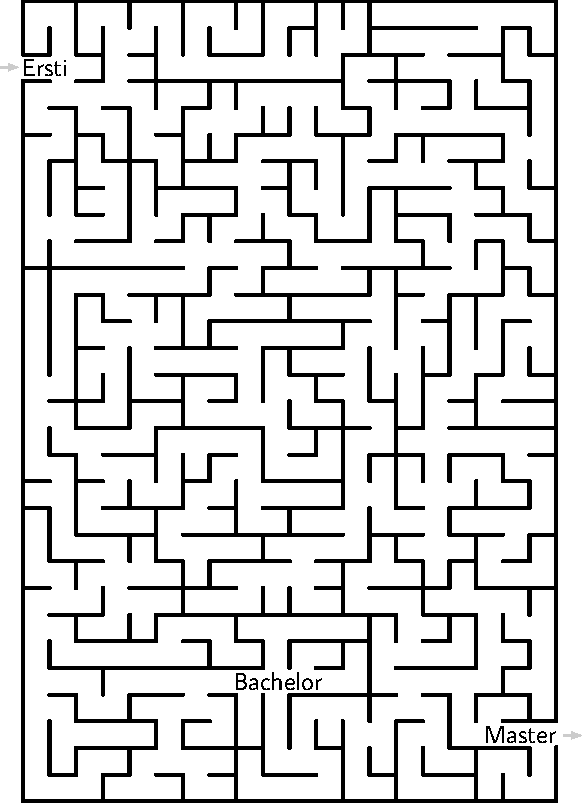
\includegraphics[width=\textwidth, height=0.38\textheight]{res/bachelor_master_labyrinth.pdf}
\end{center}

\clearpage

\section[Bachelor-Studiengang Physik]{Bachelor-Studiengang Physik\\(und Studienrichtung Scientific Instrumentation)}
\begin{multicols}{2}
\begin{quote}
	\textit{Die Wissenschaft ist nichts als das Abbild der Wahrheit.}
	
	\hfill--- Francis Bacon
\end{quote}

Wie euer Studium abläuft, könnt ihr in der jeweiligen Prüfungsordnung nachlesen. Am Besten fangt ihr mit der neuesten Prüfungsordnung an, und hangelt euch, falls der einleitende Absatz euch auf ältere Ordnungen verweist, daran entlang. Ansich ist die Prüfungsordnung zwar gut lesbar, aber nicht unbedingt kurz, sodass dieser Artikel einmal die wesentlichen Punkte eurer aktueller Prüfungsordnung (der Bachelor-Prüfungsordnung vom Sommersemester 2020) zusammenfasst.

Entgegen §2 der Prüfungsordnung (PO) ist ein Bachelor in der Physik übrigens praktisch \emph{kein} berufsqualifizierender Abschluss - die Wirtschaft akzeptiert den Abschluss in der Physik häufig erst ab einem Master.

\subsection{Modularisierung}
Das Studium gliedert sich in Module.
Ein Modul ist eine inhaltlich zusammenhängende Einheit aus mehreren Studienleistungen wie Vorlesung, Übung, Seminar, Praktikum oder Ähnlichem.
Nach dem European Credit Transfer System~(ECTS) werden Module mit Leistungspunkten (LP; manchmal auch Credit~Points, CP) gewichtet.
Ein LP entspricht dabei einem Studienaufwand von \SI{30}{\hour}, wobei hier Präsenz- und Selbststudium gemeint ist.

Der Bachelor benötigt \SI{180}{\LP}, wobei die zu belegenden Module kaum Wahlfreiheit lassen.
Einzig das Nebenfach (Modul "Fachübergreifende Studien") und die Wahl vereinzelter Kurse wird den Studierenden überlassen.
Daher lässt sich der Studienverlaufsplan für alle recht genau angeben.
Aufgrund der bisher genannten Probleme ist dieser jedoch mit Vorsicht zu genießen, da die Prüfungsordnung immer mal wieder angepasst wird, um das Studium und die Studienorganisation wieder zu vereinfachen.
Über derartige Wechsel wird euch aber auch die Fachschaft informieren.

\subsection{Studienverlauf und Inhalte}
\subsubsection{Erstes Studienjahr}
"Physik~I" ist eine Vorlesung mit Übung.
Hier werden 6~Semesterwochenstunden (SWS) Vorlesung besucht und es finden 4~SWS Übung statt, wobei in den Übungen Anwesenheitspflicht besteht.
Die wöchentlichen Übungszettel zu dieser Vorlesung müssen bearbeitet werden und bei einer erfolgreichen Bearbeitung von \SI{50}{\percent} der Übungsaufgaben wird man zur Modulabschlussprüfung (dreistündige Klausur) zugelassen.
In diesem Modul werden grundlegende Methoden der Physik sowie die klassische Mechanik gelehrt.
Außerdem wird in die relativistische Mechanik eingeführt.

"Mathematik für Physiker~I" ist auch eine Vorlesung (4~SWS) mit Übung (2~SWS), gehört jedoch zum Modul "Mathematische Grundlagen", welches auch die Vorlesung "Mathematik für Physiker~II" beinhaltet.
Die Klausur zu Mathe~I ist nur eine Studienleistung, kann also beliebig oft wiederholt werden und geht nicht in die Bachelor-Note ein.
Wie bei Physik~I auch müssen die Übungen besucht und bestanden werden.

\vspace{\fill}

\fibelimgtext[above right]{
	\includegraphics[width=\columnwidth]{res/xkcd/730_circuit_diagram.png}
}{\url{https://xkcd.com/730}}

% vergleiche auch Tabelle im Artikel Bachelor_Geophysik.tex
\begin{table*}
% Der Befehl \fibnl ist ein Zeilenumbruch
\let\fibnl=\par
% Länge \fibtemp ist die Breite einer Spalte in der Tabelle
% (außer Spalte mit den Semestern)
\setlength{\fibtemp}{0.195\textwidth}
% Mehrfachzeilen (horizontal) zentrieren
\renewcommand{\multirowsetup}{\centering}

\begin{tabularx}{\textwidth}{| X | *{4}{>{\centering\arraybackslash}m{\fibtemp}|}}
\hline
\textbf{Semester} & \multicolumn{4}{c|}{\textbf{Module im B.\ Sc.\ Physik}}
\\ \hline
1.\ (WS) &
	Physik~I\fibnl
	\SI{14}{\LP} (PM) &
	&
	\multirow{2}[5]{\fibtemp}{Mathematische Grundlagen\fibnl
		\SI{16}{\LP} (PM)} &
	\multirow{3}[5]{\fibtemp}{Fachübergreifende Studien\fibnl
		\SI{18}{\LP} (WPM\textsuperscript{*})}
\\ \cline{1-3}
2.\ (SS) &
	Physik~II\fibnl
	\SI{14}{\LP} (PM) &
	\multirow{3}[5]{\fibtemp}[-1ex]{Physikalisches Grundpraktikum\fibnl
		\SI{13}{\LP} (PM)} &
	&
\\ \cline{1-2}\cline{4-4}
3.\ (WS) &
	Physik~III\fibnl
	\SI{14}{\LP} (PM) &
	&
	Integrationstheorie\fibnl
	\SI{8}{\LP} (PM) &
\\ \cline{1-2}\cline{4-5}
4.\ (SS) &
	Atom- und Quantenphysik\fibnl
	\SI{10}{\LP} (PM) &
	&
	\multirow{2}[5]{\fibtemp}{Computational Physics\fibnl
		\SI{10}{\LP} (PM)} &
	Messtechnik und Signalverarbeitung\fibnl
	\SI{8}{\LP} (PM)
\\ \cline{1-3}\cline{5-5}
5.\ (WS) &
	Struktur der Materie\fibnl
	\SI{14}{\LP} (PM) &
	\multirow{2}[5]{\fibtemp}{Physikalisches Praktikum für Fortgeschrittene\fibnl
		\SI{12}{\LP} (PM)} &
	&
	\multirow{2}[5]{\fibtemp}[-1ex]{Quantentheorie und Statistische Physik\fibnl
		\SI{16}{\LP} (PM)}
\\ \cline{1-2}\cline{4-4}
6.\ (SS) &
	Bachelorprojekt
	\SI{13}{\LP} (PM)	&
	&
	&
\\ \hline
\end{tabularx}

\framebox[\textwidth]{
\begin{minipage}{0.95\textwidth}
\centering
PM: Pflichtmodul; WPM: Wahlpflichtmodul

\raggedright
\textsuperscript{*}: Fachübergreifendes Modul, "das in einer sinnvollen Beziehung zum Studium der Physik steht oder der Berufsbefähigung dient"
\end{minipage}
}
\end{table*}

% \newpage statt \clearpage, damit die Tabelle nicht auf einer eigenen Seite
% landet
\newpage

Das Modul "Fachübergreifende Studien" (Nebenfach im Umfang von \SI{18}{\LP}) kann frei aus einer vorgegebenen Auswahl getroffen werden.
Diese vorgefertigten Module sind:
\begin{itemize}[parsep=0.7ex]
	\item Einführung in die Informatik
	\item Geophysik
	\item Chemie (Grundlagen / Anorganische und Organische Chemie)
	\item Philosophie für Physiker
	\item Mathematik
	\item Theoretische Grundlagen der Psychologie
	\item Einführung in die Betriebswirtschaftslehre
	\item Einführung in die Volkswirtschaftslehre
	\item Spanisch für Naturwissenschaftler
	\item (Deutsch als Fremdsprache)
\end{itemize}
Man kann auch durch Absprache mit dem Studiendekan ein mit der Physik verbundenes Modul in anderen Fachbereichen zusammenstellen.

Im zweiten Semester wird "Physik~II" belegt.
Es wird eine Vorlesung (6~SWS + 2~SWS Übung) über Thermodynamik und Elektromagnetismus sowie eine Vorlesung "Theoretische Ergänzungen" (2~SWS + 1~SWS Übung) über analytische Mechanik gehört. Hinzu kommt eine Einführungsvorlesung zu experimentellem Arbeiten (1~SWS + 2~SWS Übung) zur Vorbereitung auf das Grundpraktikum.

Nach jedem Studienjahr hat man durchschnittlich \SI{60}{\LP} gesammelt.
Falls bestimmte Prüfungen nicht bestanden wurden, wird in der Regel zu einem späteren Zeitpunkt im Semester eine Nachklausur angeboten.
Eine andere Möglichkeit ist es, die Prüfung ein Jahr später zu wiederholen.
Jedoch muss man nach je nach Modul drei bis vier nicht bestandenen Versuchen das Studium abbrechen (dies ist eine der Verschärfungen, die es im Diplomstudium nicht gab; siehe PO BSc. Physik, §16 (2)).
\subsubsection[Zweites Studienjahr]{\hspace{-1.5em}Zweites Studienjahr}
\iffalse
% \intextsep: Abstand vor/nach dem Bild bei wrapfigure
\setlength{\intextsep}{1mm}
\begin{wrapfigure}[9]{r}[5mm]{0cm}
%	\scriptsize
	\raisebox{0pt}[\dimexpr\height - 6mm\relax]{%
		\fibelimgtext[above right]{
			\includegraphics[width=4.7cm]{res/xkcd/755_interdisciplinary.png}%
		}{\url{https://xkcd.com/755}}%
	}
\end{wrapfigure}
\fi
Im zweiten Studienjahr werden "Physik III" mit zugehörigen Theoretischen Ergänzungen (Vorlesung und Übung, \SI{14}{\LP}) und "Integrationstheorie" (Mathe für Physiker~III, \SI{8}{\LP}) gehört.
Außerdem beginnt der experimentelle Teil des "Physikalischen Grundpraktikums", bei dem pro Woche ein Versuch im Labor durchgeführt und protokolliert wird.

Im vierten Semester werden dann "Atom- und Quantenphysik" (inoffiziell auch "Physik~IV" genannt) und "Messtechnik und Signalverarbeitung", wo zum ersten Mal das Modul durch eine mündliche Prüfung abgeschlossen wird, gehört.
Im ersten Teil des Moduls "Computational Physics" erlernt man in einer Vorlesung das (wissenschaftliche) Programmieren mit der Programmiersprache Fortran.
Auch das Grundpraktikum setzt sich in diesem Semester fort.

\subsubsection{Drittes Studienjahr}
Das letzte Jahr des Bachelors eignet sich insbesondere zum Austausch mit diversen Partneruniversitäten (siehe Erasmus).
In diesem Studienjahr werden dann in Münster oder an der Partneruniversität äquivalente Kurse zu "Struktur der Materie" (Vorlesungen: Physik der kondensierten Materie, Kern- \& Teilchenphysik, Astrophysik \& Kosmologie; außerdem ein Seminar) besucht, sowie das Modul "Physikalisches Praktikum für Fortgeschrittene" (das sogenannte "F-Praktikum") belegt.
Der Theorieanteil wird durch das Modul "Quantentheorie und Statistische Physik" mit den gleichnamigen Vorlesungen abgedeckt.
Außerdem fällt der zweite Teil des Moduls "Computational Physics" in das fünfte Semester, in welchem die Wahl zwischen der weiterführenden Vorlesung zu Computational Physics, einem Computerpraktikum in der Angewandten Physik, einem Praktikum wie der interdisziplinären "Nichtlinearen Modellierung in den Naturwissenschaften" oder auch einem Kurs an der WWU IT gewählt werden kann.

\subsubsection{Benotung}
Die Benotung der einzelnen Module und deren Gewichtung für die Bachelornote wurde in den letzten Jahren immer wieder durch neue Prüfungsordnungen angepasst.
Im Allgemeinen orientiert man sich dabei an den Leistungspunkten eines Moduls im Verhältnis zu den insgesamt zu erreichenden \SI{180}{\LP}.
In der neuesten Prüfungsordnung gehen die beste der zwei Noten der Module Physik~I und II mit je \SI{10}{\percent} gewichtet in die Endnote ein. Hinzu kommt die Note des Moduls Physik~3 mit weiteren \SI{10}{\percent}.
Das Modul Grundlagen der Mathematik (Klausur Mathe~II) und Integrationstheorie (Klausur Mathe~III) gehen mit jeweils \SI{5}{\percent} in die Endnote ein.
Ihr müsst euch also erst einmal keine Sorgen machen, wenn die ersten Klausuren noch nicht so gut laufen.
Das Modul Fachübergreifende Studien wird mit weiteren \SI{10}{\percent} gewichtet.
Die Note des Grundpraktikums geht mit \SI{4}{\percent} in die Bachelornote ein.

Die Prüfungslast hat insgesamt in den letzten Jahren wieder abgenommen, wobei immer noch viele Module mehr geprüft werden als vor der Umstellung, was zu mehr Stress und Druck führt.
Wir konnten aber erreichen, dass die Anzahl der Versuche für eine Klausur (MAP) inzwischen auf vier erhöht wurde!
Außerdem kann man sich mittlerweile in einem zweiten Versuch verbessern, selbst wenn man die Klausur im ersten Anlauf bereits (aber evtl.\ nicht mit einer guten Note) bestanden hat.

Weitere Informationen sind auf der Homepage des Fachbereichs (\url{https://www.uni-muenster.de/Physik}) und in der Prüfungsordnung des Bachelor Physik (diese gibt es auch auf der Homepage) zu finden.

\fibelsig{Friedrich, Simon, Benedikt B.}
\end{multicols}

\section{Bachelor-Studiengang Geophysik}
\begin{multicols}{2}
Jedem, der schon einmal auf WG-Partys, Einführungskursen, Kennenlern-Spielen oder Ähnlichem herumstand, wird früher oder später die Frage gestellt "Und was studierst du?".
Gibt man als Antwort schlicht und einfach Geophysik, erntet man meist nur fragende Blicke und ein "Aha, interessant\dots\ Und was ist das?".
Hier kommen auch langjährige Geophysik-Studenten oftmals ins Grübeln und eine Antwort der Art "Wir gucken uns Erdbeben an und das Erdmagnetfeld und die Ozeane und so." ist für beide nicht sehr zufriedenstellend.
Was macht man also in der heutigen Zeit, wenn man ein Wort hört, das man nicht kennt? Man schaut natürlich bei Wikipedia nach.
Frei übersetzt von der englischen Seite findet man dort:
\vspace*{-0.5cm}
\begin{quote}
	\textit{Geophysik, eine Hauptdisziplin der Geowissenschaften und eine Teildisziplin der Physik, ist die Erforschung der gesamten Erde durch quantitative Untersuchung der physikalischen Eigenschaften.}
\end{quote}

Auch wenn dies nur eine der vielen gängigen Definitionen ist (und man sich hierüber auch streiten kann), kommen wir der Sache schon etwas näher.
Die Geophysik gehört also vom Forschungsobjekt her gesehen zu den Geo- oder Erdwissenschaften, von der Wissenschaftsmethodik her jedoch zur Physik.
Dies ist auch der Grund dafür, dass Geophysik in Deutschland teilweise in physikalischen (wie in Münster) als auch in geowissenschaftlichen Fachbereichen angesiedelt ist.

Es geht dabei um Fragestellungen, wie Erdbeben entstehen und wie sich seismische Wellen durch die Erde ausbreiten, was man dadurch über den inneren Aufbau der Erde lernen kann, warum die Erde in Japan häufiger und stärker bebt als in Deutschland, wie die Erde in ihrem Inneren aufgebaut ist, warum, woher und wohin sich die Erdplatten bewegen, wie der Wasserkreislauf der Meere entsteht, wie sich das Klima entwickelt, ob die Kompassnadel in Münster auch wirklich exakt nach Norden zeigt, ob man in Greven in 50~Jahren seinen Badeurlaub buchen kann, warum sich das Magnetfeld der Sonne alle 11~Jahre umpolt, wie schnell sich die Gletscher in der Antarktis bewegen und noch vieles mehr.

%\iffalse
\begin{tikzpicture}[remember picture, overlay]
	\node[inner sep=0, yshift=2.6cm] at (current page.center)
	{\includegraphics[width=5cm]{res/geophysik_erde.pdf}};
\end{tikzpicture}
\parshape=10
0cm \columnwidth
0cm \columnwidth
0cm \columnwidth
0cm \columnwidth
0cm \columnwidth
0cm \columnwidth
0cm 7.5cm
0cm 7.1cm
0cm 6.7cm
0cm 6.6cm
%\fi
Zu guter Letzt existieren die praktischen Anwendungen der Geophysik, die sich eigentlich immer darum drehen, wie man Ressourcen in der Erde aufspüren kann, ohne hineinzubohren (denn das ist unvorstellbar teuer).
Dabei kann es sich um Öl, Gas, Grundwasser, Salz, Erze, oder Ähnliches handeln.
Darüber hinaus gibt es noch andere Gebiete wie die Archäometrie (d.\,h.\ Geophysik in Verbindung mit Archäologie) oder das Aufspüren von Körpern im Boden, wie z.\,B.\ Bomben oder Leitungen.

%\iffalse
\parshape=11
0cm 6.6cm
0cm 6.8cm
0cm 7.0cm
0cm 7.4cm
0cm 8.0cm
0cm \columnwidth
0cm \columnwidth
0cm \columnwidth
0cm \columnwidth
0cm \columnwidth
0cm \columnwidth
%\fi
Wie läuft das Geophysik-Studium nun genau ab.
Das könnt ihr ganz genau in der Prüfungsordnung nachlesen.
Diese wird auch gelegentlich mal geändert, sodass die Leute in den Semestern über euch vielleicht etwas andere Vorlesungen hören mussten als ihr.
Die Fachschaft Geophysik hat zum Glück bei den Änderungen der Prüfungsordnung ein Wörtchen mitzureden, sodass die Änderungen meist zu Gunsten der Studierenden sind.
Die aktuellste Version findet man immer als Link auf der Geophysik-Homepage:
\begin{center}
	\url{https://www.uni-muenster.de/Physik.GP}
\end{center}

Los geht es im ersten Semester mit der Vorlesung "Einführung in die Geophysik".
Darin wendet man bereits die in Physik und Mathematik erlernten Methoden auf geophysikalische Fragestellungen an.
Die Inhalte überschneiden sich dabei zwar teilweise mit denen der Vorlesung "Die Erde", welche von Professoren der geowissenschaftlichen Institute gehalten wird, was jedoch nicht weiter schlimm ist.
Man betrachtet so die gleichen Themen sowohl aus geologischer als auch aus physikalischer Sicht.
Wie man dem Studienverlauf (siehe unten) entnehmen kann, hört man jedoch genau wie alle Physik-Bachelor-Studenten das volle Physik- und Mathe-Programm in den ersten drei Semestern.
Erfahrungsgemäß nehmen diese Vorlesungen und die dazugehörigen Übungen mit Abstand am meisten Zeit in Anspruch, sodass man hier relativ viel zu tun hat.
Noch ein Tipp zu den Physik- und Mathe-Übungsgruppen: Es kann passieren, dass sich diese Termine mit Vorlesungen aus der Geophysik der den Geowissenschaften überschneiden.
Falls dies der Fall ist, sollte man versuchen, die Termine für die Übungen in Physik umzulegen (diese werden in der ersten Vorlesungswoche festgelegt).

%\iffalse
\parshape=24
%0cm \columnwidth
0cm \columnwidth
0cm \columnwidth
0cm \columnwidth
0cm \columnwidth
0cm \columnwidth
0cm \columnwidth
0cm \columnwidth
0cm \columnwidth
0.8cm \dimexpr\columnwidth - 0.8cm
1.6cm \dimexpr\columnwidth - 1.6cm
\dimexpr\columnwidth - 7.2cm 7.2cm
\dimexpr\columnwidth - 6.8cm 6.8cm
\dimexpr\columnwidth - 6.7cm 6.7cm
\dimexpr\columnwidth - 6.6cm 6.6cm
\dimexpr\columnwidth - 6.6cm 6.6cm
\dimexpr\columnwidth - 6.7cm 6.7cm
\dimexpr\columnwidth - 6.8cm 6.8cm
\dimexpr\columnwidth - 7.2cm 7.2cm
\dimexpr\columnwidth - 7.7cm 7.7cm
0cm \columnwidth
0cm \columnwidth
0cm \columnwidth
0cm \columnwidth
0cm \columnwidth
%\fi
Im zweiten Semester lernt man in "Einführung in die geophysikalische Datenverarbeitung" die in den Naturwissenschaften häufig verwendete Programmiersprache Fortran kennen.
Auch hier muss zunächst gesagt werden: Keine Panik! Auch wer noch nie unter Linux-/Unix-Systemen gearbeitet und noch nie vorher etwas programmiert hat, kommt hier klar.
Man fängt wirklich von null an.
Zusätzlich werden vom Rechenzentrum~(ZIV) in den Semesterferien etliche Kurse angeboten.
PC-Arbeitsplätze stehen jedem Studenten der Geophysik in den beiden CIP-Pools im Institut immer zur Verfügung.
Generell wird in der Geophysik sehr exzessiv am Computer gearbeitet.
Ein Grund dafür ist, dass die Datenmengen so riesig sind, dass eine andere Möglichkeit der Bearbeitung gar nicht vorhanden ist.
Der andere Grund ist, dass man in Tiefen größer als \SI{10}{\km} technisch gar nicht mehr vordringen kann und die Physik in Gegenden wie dem Erdmantel oder Erdkern durch numerische Computermodelle simuliert wird.

Außerdem beginnt man in diesem Semester mit einer Vorlesung zur angewandten Geophysik, in welcher vier verschiedene Geländemessungen durchgeführt werden und diese Vorlesung wird im drittem und viertem Semester weiter fortgesetzt.
Man lernt die theoretischen Grundlagen der typischen geophysikalischen Untersuchungsmethoden wie Gravimetrie, Magnetik, Radar oder Geoelektrik kennen.
Zwischen dem vierten und fünften Semester nimmt man am internationalen Feldkurs teil.
Dies ist eine Exkursion, in deren Genuss nur Geophysik-Studenten kommen.
Er findet in der vorlesungsfreien Zeit in Zusammenarbeit mit Universitäten aus Edinburgh und Paris statt.
Dort lernt man erneut die in den Vorlesungen behandelten Methoden mit all ihren Gerätschaften kennen.
Der Feldkurs ist darüber hinaus eine tolle Möglichkeit, Studierende aus dem Ausland kennenzulernen und Kontakte zu knüpfen.
Der Feldkurs findet immer im Wechsel in England, Frankreich oder Deutschland statt.
Ab dem vierten und fünften Semester wird es auch in der Physik etwas angewandter
Zunächst lernt man im Modul Experimentelle Übungen~I die Experimentalphysik näher kennen.
Man sitzt dabei von Woche zu Woche in einem Raum, baut ein Experiment auf, misst Daten und wertet diese in einem Protokoll aus.
Der praktische Teil der Geophysik ist dagegen deutlich erfrischender.
Außerdem werden die mathematischen Kenntnisse vertieft und auf rein geophysikalische Probleme angewandt und ab dem vierten Semester wird sich auch mehr mit der Seismologie beschäftigt, denn im vierten und fünften Semester beginnen auch die Vorlesung zu diesem Bereich der Geophysik.
Ab dem vierten Semester kann man in den Geowissenschaften wählen, welchen Schwerpunktbereich einen am meisten interessiert. 
Im fünften Semester werden auch Kontinuumsmechanik und spezielle Anwendung von geophysikalischen Programmen gelehrt. Außerdem ist ein Seminar zu absolvieren.

Im abschließenden sechsten Semester stehen die Anfertigung der Bachelorarbeit sowie die, wenn nicht schon vorher erledigten, Allgemeinen Studien, an. Bei den Allgemeinen Studien kann man aus einer großen Auswahl von Kursen aus den Bereichen Planetologie, Chemie, Klimatologie, Sprachen und noch vielem mehr auswählen. Im Seminar lernt man, deutsch- und englischsprachige Vorträge über wissenschaftliche Themen zu halten. Auch hier: keine Panik! Auch wer der englischen Sprache nicht ganz so mächtig ist, wie Leute, die ein Auslandssemester verbracht haben oder Englisch-LK hatten, wird hier gut betreut. Es gibt in der Geophysik leider ohnehin nicht besonders viele deutsche Fachbücher, sodass man hier schon von Anfang an auch mal in ein englisches Buch reinschauen muss. Diese sind alle in unserer Bibliothek im Institut vorhanden und können dort eingesehen und teilweise auch ausgeliehen werden.


Ein letzter, ultimativer Tipp: Als Geophysik-Student kann man an dem \emph{Geophysikalischen Aktions-Programm}, kurz GAP, teilnehmen.
Dies ist ein jährliches Treffen, welches von und für Studenten organisiert wird und jedes Mal in einer anderen Stadt stattfindet.
Bei bis zu 100~Teilnehmern aus Deutschland, Polen und Österreich kommt beim ersten Abend auf der Icebreaker-Party internationales Flair auf.
Der zweite Tag besteht meist aus Exkursionen zu interessanten Orten in oder um die gastgebende Stadt herum.
Am dritten und letzten Tag stellen sich Institut und Professoren vor und es werden Vorträge von Wissenschaftlern und Sponsoren (also potenziellen Arbeitgebern) gehalten.
% XXX Jedes Jahr GAP-Termine/-Orte aktualisieren!
Nachdem das GAP zuletzt im September 2021 in Kiel war, findet das nächste hoffentlich 2022 in Berlin statt.

\fibelsig{Kevin}
\end{multicols}


\begin{table}[h]
    \centering
    \begin{tabular}{|c|c|c|c|c|c|c|}
        \hline
        \textbf{Semester} & \multicolumn{6}{c|}{\textbf{Module im B.\ Sc.\ Geophysik}}
        \\ \hline
       \multirow{3}{1cm}{1. (WiSe)} & \multirow{6}{2.3cm}{Geophysik I \footnotesize 12~LP}& \multirow{3}{2.1cm}{}&\multirow{12}{2cm}{} & \multirow{3}{1.8cm}{Physik I \footnotesize 14~LP}& \multirow{6}{2cm}{Grundlagen der Mathematik \footnotesize 16~LP} & \multirow{3}{1.9cm}{Geowissen\-schaften~I \footnotesize 4~LP} \\
       &&&&&&\\
       &&&&&&\\
        \hhline{-~~~-~-}
         \multirow{3}{1cm}{2. (SoSe)} & &\multirow{6}{2cm}{}&  &\multirow{3}{1.8cm}{Physik II \footnotesize 14~LP} & &\multirow{3}{2cm}{}\\
         & & & & & &\\
         &&&&&&\\
         \hhline{--~~---}
         \multirow{3}{1cm}{3. (WiSe)} &\multirow{6}{2.3cm}{Geophysik~II \footnotesize 13~LP} & &&\multirow{3}{1.8cm}{Physik III \footnotesize 14~LP} & \multirow{3}{2cm}{Integrations\-theorie \footnotesize 8~LP} &\multirow{3}{1.9cm}{Geowissen\-schaften~I \footnotesize 4~LP}\\
         & & & & & &\\
         &&&&&&\\
         \hhline{-~-----}
         \multirow{3}{1cm}{4. (SoSe)} & &\multirow{6}{2.3cm}{Geophysik~IV \footnotesize 9~LP}& \multirow{3}{2.3cm}{Geophysik~III \footnotesize 10~LP} &\multirow{6}{1.8cm}{Physik: Exp. Übungen~I \footnotesize 8~LP} &\multirow{9}{2cm}{Fachüber\-greifende Studien \footnotesize 10-14~LP} &\multirow{9}{1.9cm}{Geowissen\-schaften~II \footnotesize 11-15~LP}\\
         & & & & & &\\
         &&&&&&\\
         \hhline{--~-~~~}
          \multirow{3}{1cm}{5. (WiSe)} &\multirow{6}{2.1cm}{Geophysik~VI \footnotesize 7~LP} & &\multirow{3}{2.3cm}{Geophysik~V \footnotesize 9~LP}& & &\\
         & & & & &&\\
         &&&&&&\\
         \hhline{-~---~~}
         \multirow{3}{1cm}{6. (SoSe)} & &\multirow{3}{2.1cm}{Bachlor\-projekt \footnotesize 13~LP}&&&&\\
         & & & & & &\\
         &&&&&&\\
         \hline
    \end{tabular}

    \label{tab:my_label}
\end{table}


\clearpage

\section[Lehramtsstudium (2-Fach-Bachelor) für Gymnasien \& Gesamtschulen bzw. Berufskollegs]{Lehramtsstudium (2-Fach-Bachelor) für Gymnasien \& Gesamtschulen bzw. Berufskollegs}

\begin{multicols}{2}
An dieser Stelle soll der Ablauf des 2-Fach-Bachelors kurz erläutert werden. Dieser beinhaltet neben dem Fach Physik auch noch weitere Elemente wie euer Zweitfach und die Bildungswissenschaften.
\subsection*{Module}
Innerhalb des Studiums werden Vorlesungen, Übungen und Seminare in Modulen zusammen gefasst, die dann in Modulabschlussprüfungen abgeschlossen werden. In den ersten drei Semestern finden die Modulabschlussprüfungen als schriftliche Klausuren statt, danach sind es vor allem mündliche Prüfungen. Die Noten dieser Prüfungen gehen alle in eure spätere Endnote mit ein. Eine Ausnahme stellen die Klausuren in Physik 1 und 2 dar, hier zählt nur die bessere der beiden Noten. Voraussetzung ist dabei selbstverständlich das Bestehen beider Module. Außerdem ist es leider nicht möglich die Modulabschlussprüfungen beliebig oft zu wiederholen, deswegen gibt es in den Klausuren in Physik 1 bis 3 vier Versuche und in allen weiteren nur drei.
\subsection*{Die Grundmodule}
In den ersten drei Semestern belegt ihr die grundlegenden Module für das Physikstudium: Dynamik der Teilchen und Teilchensysteme (Physik 1), Thermodynamik und Elektromagnetismus (Physik 2) und Wellen und Quanten (Physik 3). Die Module decken sich im Prinzip mit denen der 1-Fach-Bachelor (1FB) und bestehen aus drei Vorlesungsterminen und zwei (für Physik 1) bzw. einem (Physik 2 \& 3) Übungstermin pro Woche. In der Übung müsst ihr wöchentlich Aufgaben zum Stoff der Vorlesung lösen und insgesamt die Hälfte der Punkte erreichen, um zur abschließenden Klausur zugelassen zu werden. Die Klausur orientiert sich dann ebenfalls an den Inhalten der Übungsaufgaben. Im Unterschied zum 1FB gibt es für euch in Physik 1 noch ein spezielles Mathetutorium. Dieses besteht aus einem verpflichtenden, aber unbenoteten, Test zu Beginn des Semesters und einem wöchentlichen, freiwilligen Tutorium, welches allerdings sehr hilfreich für die Übungen ist. In Physik 2 und Physik 3 hören die 1-Fach-Bachelor zusätzlich noch Theoretische Ergänzungen (TE), die ihr nicht belegen müsst.\\
Im dritten und vierten Semester muss außerdem noch das Modul Experimentelle Übungen, manchmal auch Grundpraktikum genannt, absolviert werden. Innerhalb dieses Moduls werdet ihr alle zwei Wochen eigene Experimente durchführen und diese in Versuchsberichten auswerten, die bewertet werden und eure Modulnote ergeben.
\subsection*{Weitere Module}
Nach den oben genannten grundlegenden Modulen wird im vierten Semester das Modul Atom- und Quantenphysik absolviert. Dieses ist mit Vorlesung und Übung genauso aufgebaut wie in den vorherigen Semestern, die Modulabschlussprüfung wird allerdings zum ersten Mal als mündliche Prüfung von circa 30-45 Minuten Länge stattfinden.\\
Das fünfte Semester widmet sich dem Modul Struktur der Materie. Es beinhaltet Vorlesungen in Kern- und Teilchenphysik, Physik der kondensierten Materie und Astrophysik und Kosmologie. Allerdings müssen nur in den ersten beiden Teilvorlesungen Übungen besucht werden. Auch dieses Modul wird durch eine mündliche Prüfung abgeschlossen.\\
Im sechsten Semester wird das Modul Messtechnik und Signalverarbeitung eingeführt. Hier müsst ihr die Kombination aus Vorlesung und Übung in den Grundlagen der Signalverarbeitung absolvieren und durch eine mündliche Prüfung abschließen.\\
Des Weiteren wird in den Semestern fünf und sechs das Modul Grundlagen der Fachdidaktik und Erkenntnistheorie absolviert. Es beinhaltet eine Vorlesung zur Einführung in die Fachdidaktik der Physik für das Lehramt Physik mit abschließender mündlichen Prüfung und ein Seminar zur Theorie, Geschichte und Kultur der Naturwissenschaften, in dem ihr eine Seminararbeit z. B. Referat oder Hausarbeit erstellen müsst.\\
Am Ende könnt ihr euch noch entscheiden, ob ihr eure Bachelorarbeit in der Physik oder in einem eurer anderen Fächer schreiben möchtet.\\
Genauere Informationen zu den Inhalten und Prüfungsleistungen der Module, sowie einen beispielhaften Studienverlaufsplan findet ihr auf der Homepage des Fachbereichs (\url{https://www.uni-muenster.de/Physik}) und in eurer jeweiligen Prüfungsordnung (diese gibt es auch auf der Homepage).
\subsection*{Bildungswissenschaften}
In den Bildungswissenschaften müsst ihr drei Pflichtmodule absolvieren, die namentlich zwar nach Lehramt für Gymnasien/Gesamtschulen (Gym/Ge) sowie Berufskolleg (BK) aufgeteilt sind, sich strukturell aber sehr ähneln. Zunächst muss das Modul Einführung in Grundfragen von Erziehung, Bildung und Schule (für Gym/Ge) bzw. Einführung in Grundfragen beruflicher Bildung (für BK) absolviert werden. Dazu gehören eine Vorlesung inklusive Tutorium und abschließender Klausur sowie ein frei wählbares Seminar mit eigener Prüfungsleistung. Dieses Modul sollte im ersten oder zweiten Semester belegt werden, wobei sich meistens das zweite Semester besser eignet. Außerdem müssen noch zwei Praktika während des Bachelors absolviert werden. Zunächst das Eignungs- und Orientierungspraktikum, in welchem ihr fünf Wochen in einer von euch gewählten schulischen Einrichtung (passend zu eurer angestrebten Schulform) hospitiert und später das Berufsfeldpraktikum über 4 Wochen, in dem ihr Berufsmöglichkeiten außerhalb des Lehramts kennen lernen sollt.  Dazu gibt es ein vorbereitendes Seminar (gegebenenfalls auch begleitend oder nachbereitend) und ihr müsst einen Praktikumsbericht anfertigen.\\
Weitere Informationen zu den Modulen sowie die Prüfungsordnung findet ihr auf den Seiten der Bildungswissenschaften (\url{https://www.uni-muenster.de/Bildungswissenschaften/}).

Das sind zunächst die wichtigsten Informationen, die ihr für die Bewältigung eures Bachelorstudiums braucht. Solltet ihr noch weitere Fragen zum Bachelor oder vielleicht sogar schon zum Master haben, könnt ihr gerne in die Fachschaft vorbei schauen. Dort hilft man euch gerne weiter. Bei grundlegenden Fragen könnt ihr auch zur Zentralen Studienberatung gehen. Außerdem empfiehlt es sich natürlich die speziellen Infoveranstaltungen für 2-Fach-Bachelor während der Orientierungswoche zu besuchen :-)


\fibelsig{Andrea, Moritz}

%\begin{center}
%	\fibelimgtext{
%		\includegraphics[width=\columnwidth, height=0.23\textheight]{res/xkcd/894_progeny.png}
%	}{\url{https://xkcd.com/894}}
%\end{center}
\end{multicols}

\begin{table}[h]
        \centering
        \begin{tabular}{|c|c|c|}
        \hline
        \multirow{2}{*}{\textbf{Semester}} & \multicolumn{2}{c|}{\multirow{2}{*}{\textbf{Module im 2-Fach-Bachelor Physik}}} \\ 
        & \multicolumn{2}{c|}{} \\
        \hline
        \multirow{3}{1cm}{1. (WiSe)} & \multirow{3}{3.5cm}{\makecell{Physik~I\\ \footnotesize 15~LP}} & \\
        &&\\
        &&\\
        \cline{1-2}
        \multirow{3}{1cm}{2. (SoSe)} & \multirow{3}{3.5cm}{\makecell{Physik~II \\ \footnotesize 10~LP}} & \\
        &&\\
        &&\\
        \hline
        \multirow{3}{1cm}{3. (WiSe)} & \multirow{3}{3.5cm}{\makecell{Physik~III \\ \footnotesize 10~LP}} & \multirow{7}{3.5cm}{\makecell{Experimentelle\\Übungen~I \\ \footnotesize 8~LP}} \\ 
        &&\\
        &&\\
        \cline{1-2}
        \multirow{4}{1cm}{4. (SoSe)} & \multirow{4}{3.5cm}{\makecell{Atom- und \\Quantenphysik \\ \footnotesize 10~LP}} & \\
        &&\\
        &&\\
        &&\\
        \hline
        \multirow{4}{1cm}{5. (WiSe)} & \multirow{4}{3.5cm}{\makecell{Struktur der\\ Materie \\ \footnotesize 27~LP}} & \multirow{8}{3.5cm}{\makecell{Grundlagen der\\Fachdidaktik und \\Erkenntnistheorie\\\footnotesize 8~LP}} \\
        &&\\
        &&\\
        &&\\
        \cline{1-2}
        \multirow{7}{1cm}{6. (SoSe)} & \multirow{4}{3.5cm}{\makecell{Messtechnik und\\Signalverarbeitung \\ \footnotesize 8~LP}} & \\
        &&\\
        &&\\
        &&\\
        \cline{3-3}
        & \multirow{3}{3.5cm}{\makecell{Bachelorarbeit \\ \footnotesize 10~LP~(WPM)}} &\\
        &&\\
        &&\\
        \hline
    \end{tabular}
    %\label{Tab.2FB_Module}
\end{table}

\clearpage

\section[Stundenplan 1.~Semester]{Dein Stundenplan im 1.~Semester}
\vspace{-0.5cm}
\subsubsection*{für 1-Fach-Bachelor-Physiker, 2-Fach-Bachelor-Physiker und Geophysiker}
\begin{minipage}{\textwidth}
% Keine Trennlinie vor Fußnoten in dieser minipage
\setfootnoterule{0cm}
% Die Länge \fibtemp ist die Breite einer Spalte in der Tabelle
% (außer Spalte mit den Zeiten)
\setlength{\fibtemp}{0.152\textwidth}
% Der Befehl \fibnl ist ein Zeilenumbruch
\let\fibnl=\par

\centering
% Verlinkung von Fußnoten im PDF klappt nicht mit tabularx :-(
% geht mit tabular, tabular*
\begin{tabular}{| >{\footnotesize}p{0.1\textwidth} | *{5}{>{\footnotesize\centering\arraybackslash}p{\fibtemp}|}}
\hline
	\textbf{Uhrzeit} &
	\textbf{Montag} &
	\textbf{Dienstag} &
	\textbf{Mittwoch} &
	\textbf{Donnerstag} &
	\textbf{Freitag}
\\ \hline
08:00--\fibnl
10:00 Uhr &
	\textbf{Physik~I\fibnl
		Übung}\footnote{Nicht der einzige mögliche Termin, aber der empfohlene. Entsprechend finden die Veranstaltungen in diversen Seminarräumen statt. Die Zuteilung der Gruppen erfolgt meistens über den LearnWeb Kurs der Veranstalltung oder in der ersten Vorlesung\label{stundenplan:multi}}\fibnl
	 &
	\textbf{Mathe für Physiker~I\footnote{Nicht für 2-Fach-Bachelor-Studenten.\label{stundenplan:mfp1}} Übung\cref{stundenplan:multi}}\fibnl
	 &
	\textbf{Physik~I Vorlesung}\fibnl
	HS~1 &
	\textbf{Physik~I\fibnl
		Übung\cref{stundenplan:multi}}\fibnl
	 &
	Informatik~I\cref{stundenplan:informatik} Übung\cref{stundenplan:multi}\fibnl
	
\\ \hline
10:00--\fibnl
12:00 Uhr &
	\textbf{Mathe für Physiker~I\cref{stundenplan:mfp1} Vorlesung}\fibnl
	HS~2 &
	\textbf{Physik~I Vorlesung}\fibnl HS~1 &
	&
	\textbf{Mathe für Physiker~I\cref{stundenplan:mfp1} Vorlesung}\fibnl
	HS~2 &
	\textbf{Physik~I Vorlesung}\fibnl
	HS~1
\\ \hline
12:00--\fibnl
13:00 Uhr &
	Chemie\footnote{Für 1-Fach-Bachelor Physik mit dem Modul Chemie als fachübergreifende Studie.
	
	Die Termine zu den Übungen werden in der Vorlesung verteilt.\label{stundenplan:chemie}} Vorlesung\fibnl
	C1 &
	Chemie\cref{stundenplan:chemie} Vorlesung\fibnl
	C1 \flushright
	&
	Chemie\cref{stundenplan:chemie} Vorlesung\fibnl
	C1 \fibnl
	\textbf{\& TUT (KP~404)}
	&
	Chemie\cref{stundenplan:chemie} Vorlesung\fibnl
	C1 &
\\ \hdashline
13--14 Uhr &
	& & & &
\\ \hline
14:00--\fibnl
16:00 Uhr &
	Informatik~I\footnote{Für 1-Fach-Bachelor Physik mit dem Modul Informatik als fachübergreifende Studie.
	
	Die Termine zu den Übungen werden in der Vorlesung verteilt.\label{stundenplan:informatik}} Vorlesung\fibnl
	M~1+M~3 &
	&
	Einführung in die Geophysik\footnote{Für 1-Fach-Bachelor Geophysik und 1-Fach-Bachelor Physik mit dem Modul Geophysik als fachübergreifende Studie.
	
	Die Termine zu den Übungen werden in der Vorlesung verteilt.\label{stundenplan:geophysik}} Vorlesung\fibnl
	HS~AP \fibnl
	\textbf{\& REP (KP~304)}&
	Informatik~I\cref{stundenplan:informatik} Vorlesung\fibnl
	M~1+M~3 &
\\ \hline
16--18 Uhr &
	& 	\textbf{REP (KP~404)}&
	& &
\\ \hline
18:00--\fibnl
20:00 Uhr &
	&
	&
	Fachschafts-Sitzung\fibnl
	IG1 87\fibnl
	(Ihr seid alle willkommen!) &
	&
\\ \hline
\end{tabular}
\vspace{-1ex}
\end{minipage}
{\footnotesize
\textbf{REP} Mathe-Repetitorium: \textit{zweistündiges, freies Angebot zum Vertiefen grundlegender Mathematik mit wöchentl.\ Themen}\\
\textbf{TUT} Tutorium: \textit{zweistündiges, freies Angebot zum Vertiefen allgemein grundlegender Themen}
}

{\small
Des Weiteren können 1-Fach-Bachelor-Studenten, die weder Chemie, Geophysik, noch Informatik als fachübergreifende Studie wählen möchten, aus folgenden vorgefertigten Modulen als fachübergreifende Studien wählen:
\begin{itemize}[nosep]
	\item Philosophie für Physiker
	\item Mathematik
	\item Theoretische Grundlagen der Psychologie
	\item Einführung in die Betriebswirtschaftslehre
	\item Einführung in die Volkswirtschaftslehre
	\item Spanisch für Naturwissenschaftler
	\item (Deutsch als Fremdsprache)
\end{itemize}
oder ein selbst zusammengestelltes fachübergreifendes Modul, bei dem der Zusammenhang zur Physik erkennbar ist, oder das zur Berufsfähigkeit dient, bestimmen.
Dies ist aber nur nach Absprache mit dem Studiendekan möglich (aktuell: Prof.\ Dr.\ Hubert Krenner, Wilhelm-Klemm-Str. 10, Raum 328 (IG1), \phonenumber{0251 83}[33621], \email{studiendekan.physik@uni-muenster.de}).
Die genauen Vorlesungs-/Übungszeiten der zusätzlichen fachübergreifenden Studien erfahrt ihr in der O-Woche von der Fachschaft Physik, direkt von der jeweiligen Fachschaft des zuständigen Fachbereiches, oder ihr schaut einfach im Vorlesungsverzeichnis (HIS~LSF, \url{https://studium.uni-muenster.de/qisserver/rds?state=wtree&search=1}) der Uni nach.
}

\clearpage

% XXX Jedes Jahr Professoren-Texte aktualisieren!
\section[Eure Profs stellen sich vor]{Eure Professoren stellen sich vor}
\textbf{Auf den folgenden zwei Seiten stellen sich eure beiden Professoren vor.
    Sie werden gemeinsam die "Physik~1" bis "Physik~3" lesen.
    Prof.\ Thiele sowie Prof.\ Wittkowski werden sich dabei um die theoretischen und Prof.\ Fallnich um die experimentellen Aspekte des Studiums kümmern.
    Zudem stellt sich Prof.\ Wulkenhaar vor, der die Vorlesungen "Mathematik für Studierende der Physik" halten wird (ebenfalls über drei Semester).
	Da diese drei Professoren euch eine Zeit lang begleiten werden, ist es durchaus interessant zu wissen, was sie gemacht haben, bevor sie an die Uni Münster kamen, und wie ihre aktuelle Forschung aussieht.}

\begin{multicols}{2}
Liebe Erstsemesterstudentinnen und -studenten, fühlen Sie sich herzlich willkommen! Wir -- also Ihr Physik-Lehr-Team 2023 bis 2025 -- freuen uns, dass Sie eine gute Wahl getroffen und sich für ein Physikstudium an der Universität Münster entschieden haben. In den nächsten drei Semestern bieten wir Ihnen die Möglichkeit, sich regelmä{\ss}ig in den Vorlesungen Physik 1 bis 3 zu treffen, um sich durch die Themenfelder Mechanik, spezielle Relativitätstheorie, Thermodynamik sowie Elektrostatik und -dynamik bis hin zur Optik führen zu lassen. Dabei werden Prof.\ Fallnich für den experimentellen sowie Prof.\ Thiele und Prof.\ Wittkowski für den theoretischen Teil verantwortlich sein. Unsere Aufgabe ist es, Ihnen zu vermitteln, wie Sie sich die Physik und die zugehörigen inneren Zusammenhänge z.B. über Symmetriebetrachtungen systematisch erarbeiten können. Hierfür werden Ihnen die oben genannten Themenbereiche sowohl in Theorie als auch Experiment mit regelmä{\ss}igem wechselseitigem Bezug zueinander nähergebracht. Zur ersten Anwendung und auch Vertiefung Ihres erlernten Wissens wird Privatdozent Kovarik zusammen mit Übungs\-gruppen\-leiter\-innen und -leitern einen Übungsbetrieb umsetzen, durch den Sie anhand ausgewählter Beispielaufgaben die fachlichen Inhalte stärker im Detail kennenlernen werden. Für die Vorbereitung und Ausführung instruktiver Experimente in der Vorlesung ist Herr Horstmann zuständig.

Damit Sie wissen, mit welchen Dozenten Sie es direkt zu tun haben werden, möchten wir uns Ihnen gern kurz vorstellen:

Prof.\ Raphael Wittkowski ist für den theoretischen Kursteil mitverantwortlich. Er arbeitet seit 2016 an der Universität Münster und forscht auf den Gebieten der Aktiven weichen Materie und der Statistischen Physik. Aktive weiche Materie besteht aus Teilchen, die sich selbstständig fortbewegen können, wie Mikroorganismen und Mikroroboter. Die Statistische Physik befasst sich mit der Beschreibung von Vielteilchensystemen. Seine Freizeit verbringt er gern in der Natur.

Prof.\ Uwe Thiele hat in den 1990ern Physik studiert, um herauszufinden, "was die Welt im Innersten zusammenhält". Nach einer ersten Tendenz in Richtung Elementarteilchenphysik, richtete sich sein Interesse aber schnell auf die Physik strukturbildender Systeme, an denen er auch heute noch mit ungebrochen großem Interesse forscht. Nach zahlreichen Forschungs- und Lehraufenthalten an verschiedenen Standorten im In- und Ausland verlagerte er vor ca.\ 10 Jahren seine Aktivitäten an die Universität Münster, wo seine Gruppe universelle Eigenschaften komplexer Nichtgleichgewichtssysteme mit analytischen und numerischen Methoden erforscht. Aufgrund vieler nichtlinear wechselwirkender Komponenten können Selbstorganisationsprozesse entstehen, die zur spontanen Entwicklung von räumlichen und zeitlichen Strukturen führen, die also nicht von au{\ss}en aufgeprägt werden. Im alltäglichen Leben zeigen sich solche Phänomene z.B. als Konvektionszellen im Milchkaffee, bei der Ausbildung von Mustern und Strukturen in der Tier- und Pflanzenwelt, und in der Dynamik von Wasserwellen, Sanddünen oder Wolkenbändern. Von gro{\ss}em aktuellem Interesse sind Tropfen komplexer Flüssigkeiten auf festen oder weichen Substraten, die Dynamik biologischer Zellen, die Entwicklung von Bakterienkolonien und allgemein die datengetriebene Modellierung.

\end{multicols}
\begin{center}

\includegraphics[width=0.6\columnwidth, height=0.25\textheight]{res/vorstellungsfotos/profs_ws23.jpg}\\
\smallskip
Gruppenfoto der Physik~1-3 Dozenten; in Ihrem Bezugssystem von links nach rechts: Carsten~Fallnich, Raphael~Wittkowski, Karol~Kovarik und Uwe~Thiele.
\end{center}

\newpage

\begin{multicols}{2}

Prof.\ Carsten Fallnich wird sich um den experimentellen Kursteil kümmern und mit Experimenten und zugehörigen Erklärungen den theoretischen Vorlesungsstoff veranschaulichen und damit weitergehend vertiefen. Er kann auf mehr als drei Jahrzehnte Wissen und Erfahrung aus Forschung und Entwicklung zurückgreifen, davon zahlreiche auch außerhalb der Universität und seit 2006 in Münster. Er ist international anerkannter Experte in der Erzeugung und Anwendung von ultrakurzen Lichtimpulsen und der nichtlinearen Optik in Wellenleitern für die zukunftsweisende Photonik, welche nahezu alle Disziplinen der modernen Physik verbindet. Neben der Arbeit an der Universität verbringt Carsten Fallnich soweit wie möglich Zeit mit der Familie, joggt, fotografiert, fährt Zweiräder mit und ohne Motor und repariert (zumindest immer mit Erkenntnisgewinn!) aus Interesse an Nachhaltigkeit und Technikverständnis fast alles, was ihm ohne reguläre Funktion unter die Finger kommt.

Priv.-Doz.~Karol Kovarik organisiert den Übungsbetrieb in den Kursen Physik 1-3. Er bietet auch verschiedene freiwillige Angebote an, um Ihnen den Einstieg in die Physik zu erleichtern und um Ihnen die Gelegenheit zu geben, zusätzliche Fragen zu den Inhalten der Vorlesungen und übungen zu stellen. Seit seiner Promotion in 2006 forscht er im Feld der Elementar- und Astroteilchenphysik. Besonders spannend findet er die Suche nach der gro{\ss}en vereinheitlichten Theorie und Versuche, die innere Struktur des Protons zu verstehen. Wenn er nachts nicht schlafen kann, fotografiert er nächtliche Landschaften und den Sternenhimmel.

Das Verständnis komplexer Phänomene, welche das Leben in unserer Welt erst interessant gestalten und an denen z.B. viele  Arbeitsgruppen am Fachbereich Physik forschen, baut -- ob Sie es uns (schon jetzt) abnehmen mögen oder nicht -- auf den Inhalten der Grundvorlesungen auf, die nun auf Sie warten. Den notwendigen Stoffumfang dazu werden Sie sich mit Interesse, Motivation und Einsatz erfolgreich selbstständig unter unserer Anleitung aneignen können; dafür wünschen wir Ihnen Durchhaltevermögen, Freude und Erfolg. Denn es wird sich später für Sie in verschiedenster Weise auszahlen, in physikalischer Weise denken und handeln zu können. Sollten dann doch noch zwischendrin Fragen offen bleiben oder Sie sich bereits für Näheres zu unseren Forschungsarbeiten interessieren, kontaktieren Sie uns gerne unter den folgenden Kontaktdaten:\\

\begin{itemize}
\item Prof.\ Dr.\ Carsten Fallnich, Institut für Angewandte Physik (AP), Büro 210, Tel.: +49\,251~83-36160, Email: \email{fallnich@uni-muenster.de} \\ \url{https://kurzelinks.de/fallnich} 

\item Prof.\ Dr.\ Uwe Thiele, Institut für Theoretische Physik (ITP), Büro 315,  Tel.: +49\,251~83-34939, Email: \email{u.thiele@uni-muenster.de} \\ \url{https://kurzelinks.de/Thiele} 

\item Priv.\ Doz.\ Dr.\ Karol Kovarik, Institut für Theoretische Physik (ITP), Büro 320, Tel.: +49\,251~83-34920, Email: \email{karol.kovarik@uni-muenster.de} \\ \url{https://kurzelinks.de/kovarik} 

\item Prof.\ Dr.\ Raphael Wittkowski, Center of Soft Nanoscience (SoN), Büro 120.024, Tel.: +49\,251~83-34529, Email: \email{raphael.wittkowski@uni-muenster.de} \\ \url{https://www.uni-muenster.de/Physik.TP/research/wittkowski} 
\end{itemize}

\begin{center}
\includegraphics[width=0.8\columnwidth]{private/res/comics/manchmal_edited.jpg}\\
{\footnotesize 
S.~Harris – \url{sciencecartoonsplus.com}
}
\end{center}

\end{multicols}

\vfill

\newpage

\begin{multicols}{2}
\begin{center}
	% 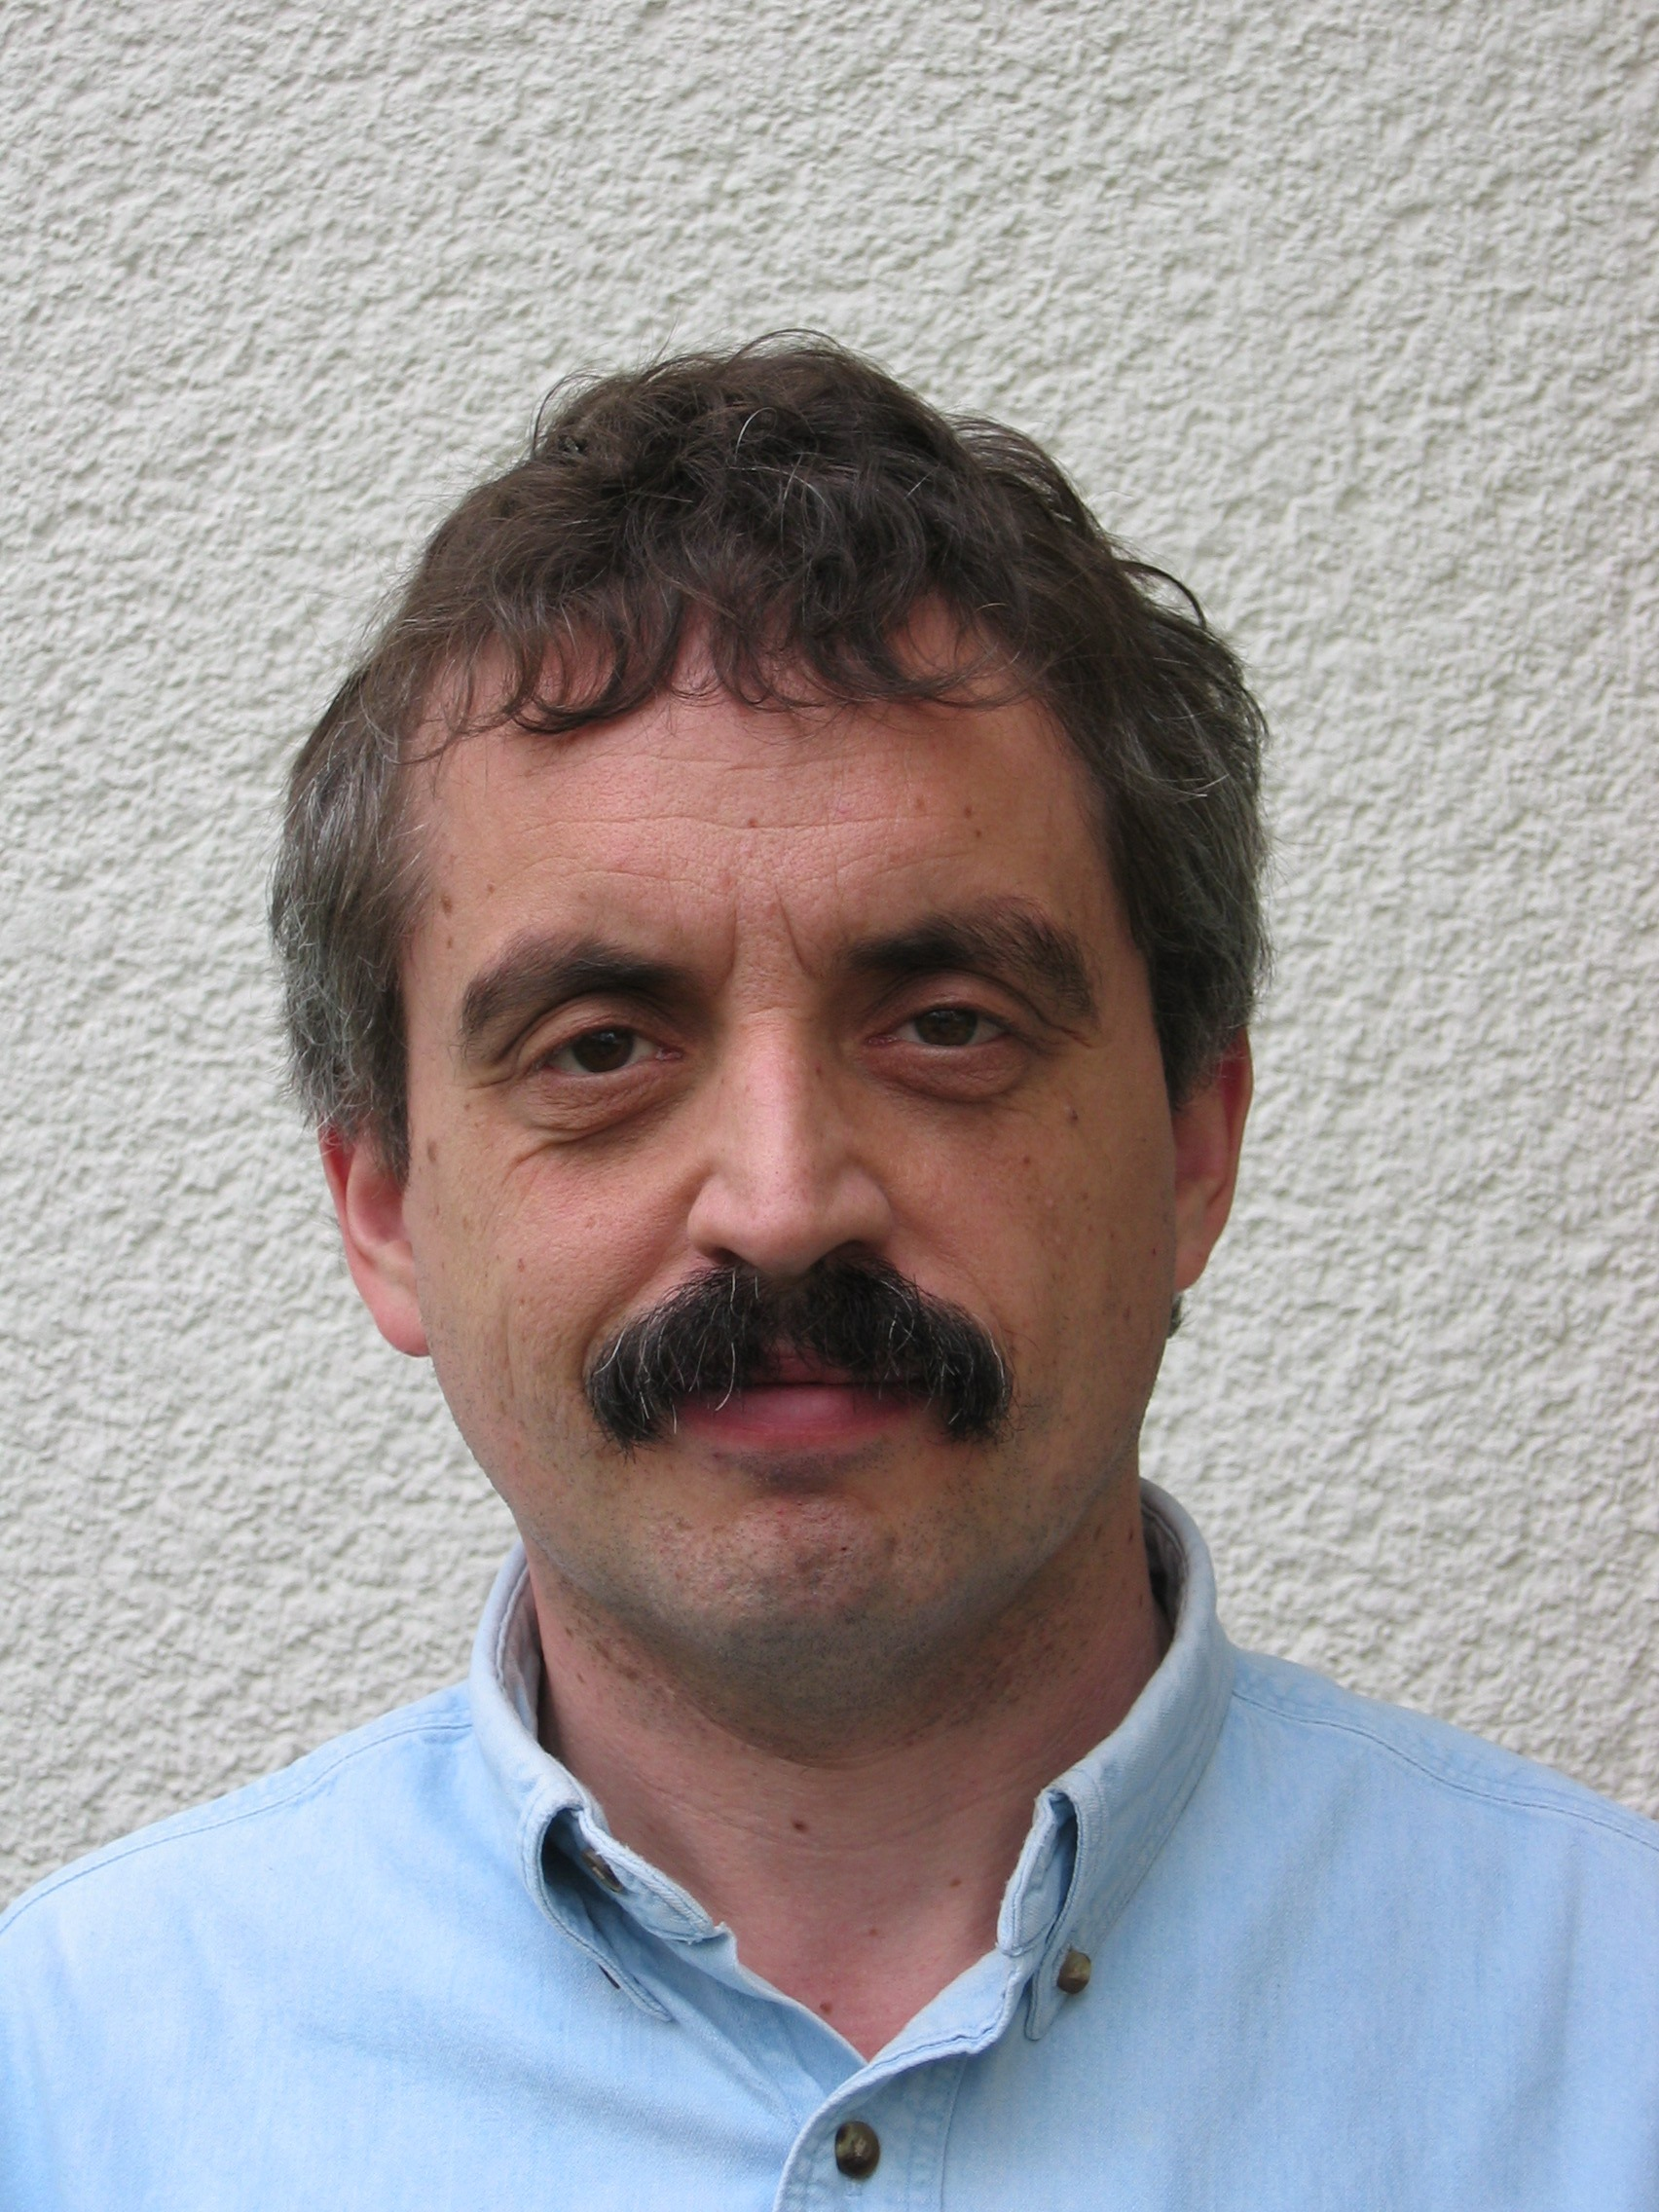
\includegraphics[width=\columnwidth, height=0.35\textheight]{res/vorstellungsfotos/wend_werner.jpg}\\
	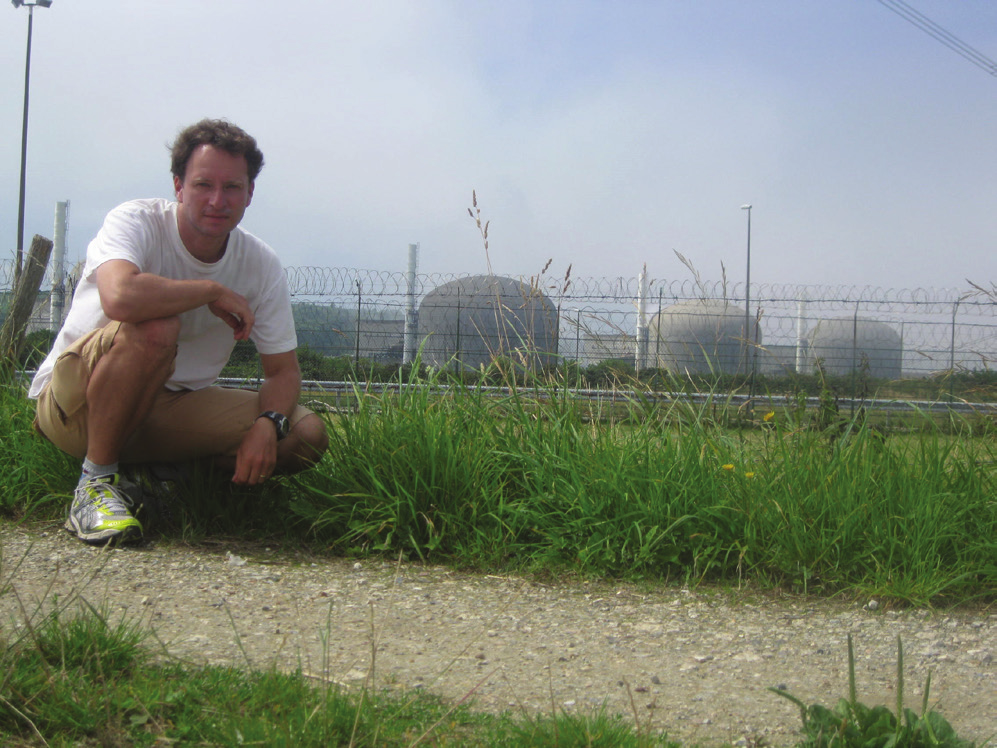
\includegraphics[width=\columnwidth, height=0.35\textheight]{res/vorstellungsfotos/wulkenhaar.png}\\
	\smallskip
 	Prof.\ Dr.\ Raimar Wulkenhaar\\
	Mathematisches Institut
\end{center}

Ich bin von der Ausbildung her Physiker, arbeite im Grenzgebiet zwischen Mathematik und Physik und bin seit 2005 Professor für Reine Mathematik am Fachbereich Mathematik und Informatik der WWU.

Die Vorlesung "Mathematik für Physiker" wird traditionell vom Mathematischen Institut veranstaltet. Es ist aus meiner Sicht eine schöne Vorlesung; mir ist aber klar, dass die meisten Studierenden das anders sehen.

Auch wenn der Stoff durchaus umfangreich ist, können wir nur einen kleinen Teil dessen behandeln, was die Physik benötigt. Es geht in der Vorlesung nicht um die Bereitstellung von Rechenwerkzeugen für die Physik; das bekommen Sie nebenbei in den Physikvorlesungen geliefert. Es geht in der Mathematik darum zu verstehen, weshalb diese Rechenwerkzeuge so und nicht anders funktionieren. Der Einstieg in die Denkweise der Mathematik ist für viele nicht leicht. Erst im Lauf der Zeit entsteht rückblickend ein gewisses Verständnis für die tiefliegenden Strukturen und Zusammenhänge der Mathematik. Im Idealfall gelangen Sie so zu einer soliden Grundlage, mit der Sie die Rechenwerkzeuge der Physik nicht nur verstehend nutzen, sondern kreativ weiterentwickeln können.


\[
\resizebox{0.45\hsize}{!}{$\displaystyle\sum_{n = 1}^\infty \frac{1}{n^2} = \frac{\pi^2}{6}$}
\]

Nun noch einige Informationen zu mir. Nach Physikstudium an der Universität Leipzig mit Abschluss als Diplomphysiker. 1994 habe ich in Leipzig auch meine Doktorarbeit geschrieben und 1997 verteidigt. Dabei ging es um die Formulierung von Modellen der Teilchenphysik im Rahmen der nichtkommutativen Geometrie. Die Ergebnisse sind rückblickend völlig unwichtig, sie haben mich aber 1998/1999 als DAAD-Postdoc nach Marseille gebracht.

Ich habe am Centre de Physique Theorique in Marseille mein Arbeitsgebiet gefunden, die Quantenfeldtheorie auf nichtkommutativen Geometrien. Vereinfacht gesagt geht es um die Frage (und ihre Konsequenzen), ob man auf beliebig kleinen Längenskalen, sagen wir $10^{-80}$\,m, noch Physik betreiben kann. Es gibt gute Gründe anzunehmen, dass das unmöglich ist, und entsprechend sollte zur Formulierung physikalischer Gesetze eine Geometrie benutzt werden, in der $10^{-80}$\,m ebenfalls sinnlos sind. Diese Nichtkommutative Geometrie wird in einer Sprache analog zur Quantenphysik beschrieben.

Seit Marseille, vor allem aber seit meiner zweiten Postdoc-Station 2000/2001 an der Universität Wien, arbeite ich an quantenfeldtheoretischen Modellen auf einer besonders einfachen nichtkommutativen Geometrie. Während meines dritten Postdoc-Aufenthalts 2002/2005 am Max- Planck-Institut für Mathematik in den Naturwissenschaften in Leipzig konnte ich mit meinem Kollegen aus Wien zusammen eine größere Hürde beseitigen. Die mathematisch rigorose Konstruktion einer 4-dimensionalen Quantenfeldtheorie auf einer nichtkommutativen Geometrie konnten wir inzwischen abschließen. Etwas analoges ist in der üblichen kommutativen Geometrie bisher nicht geglückt. Es resultierten spannende Fragen, an denen ich seitdem arbeite.

\begin{center}
	%\fibelimgtext{
		%\includegraphics[width=0.85\textwidth]{res/xkcd/435_purity.png}
	%}{\url{https://xkcd.com/435}}
 	\includegraphics[width=0.85\columnwidth]{private/res/comics/calvin_mathe.pdf}
\end{center}

\end{multicols}

\clearpage

\section[\texorpdfstring{"Penthouse oder Parkbank?"}{„Penthouse oder Parkbank?“} Wohnungssuche in Münster]{"Penthouse oder Parkbank?"\\Wohnungssuche in Münster}
\begin{multicols*}{2}
% Schriftgröße für \subsection in diesem Teil anpassen
\addtokomafont{subsection}{\normalsize}
\textbf{Nichts überstürzen und nicht aufgeben lautet die Devise.
Wohnungssuche in Münster ist ein Kapitel für sich!}

\begin{center}
	\includegraphics[width=\columnwidth]{private/res/comics/snoopy_boot_1.png}
\end{center}

Sicherlich hast du schon gemerkt, dass es in Münster weniger Wohnungen gibt, als nachgefragt werden.
Und wenn man dann endlich eine akzeptable 1-Zimmer-Wohnung gefunden hat, stürzen einen der Mietpreis oder die Nebenkosten ohne finanzielle Unterstützung der Eltern oder anderer Verwandter in den finanziellen Ruin.

Daher ist es vielleicht gerade am Anfang einfacher (besonders, wenn du in der Nähe von Münster wohnst), zu Hause wohnen zu bleiben, anstatt in Panik irgendeinen Mietvertrag als Notlösung (zu hohe Kosten/Nichtgefallen) zu unterschreiben.
Hierfür sind die Bus- und Zugverbindungen im Münsterland optimal (Siehe auch Artikel "Semesterticket").
Auch eine Anreise mit dem Fahrrad ist (bei schönem Wetter) im Münsterland aufgrund von gut geplanten Fahrradstrecken und Fahrradwegen auch kein Problem.
Natürlich ist "Hotel Mama" gerade am Anfang leichter, da so die Doppelbelastung aus neuem Studiengang und eigenem Haushalt im 1.~Semester entfällt; trotzdem solltest du dich langfristig darauf konzentrieren, auf eigenen Füßen zu stehen.

Bevor du dich von den teuren Anschaffungskosten abschrecken lässt, lass dir kurz sagen, dass der durchschnittliche Quadratmeterpreis in der Stadt Münster bei \SI{11}{\euro\per\m\squared} liegt und zu den Außenbezirken hin abfällt.
Außerdem solltest du darauf achten, dass du deine Wohnung nicht zu weit von deiner Fakultät weg planst.
So bietet sich zum Beispiel für die Fachbereiche Physik, Mathematik und Chemie der Stadtteil Gievenbeck an.

\subsection{Aller Anfang ist schwer}
Erst einmal solltest du dir darüber klar werden, welche Ansprüche und finanziellen Möglichkeiten du hast, denn gerade in Münster ist Wohnraum teuer (siehe oben).
Auch wenn in den letzten Jahren im größeren Umfang neuer Wohnraum in Form von Stadtranderweiterungen entstanden ist, hält sich das Angebot an Studi-tauglichen Wohnungen dennoch in Grenzen.
Willst du in einer WG wohnen, oder in einem kleinen Apartment?
Eine Suche nach einer passenden Bleibe in Münster, mag sie auch vielleicht etwas länger dauern, lohnt sich jedoch auf jeden Fall.
Also fang' einfach mal an.

\begin{center}
	\includegraphics[width=\columnwidth]{private/res/comics/snoopy_boot_2.png}
\end{center}

\subsection{1.~Versuch: Studentenwohnheime}
Neben dem Studierendenwerk Münster gibt es auch noch Häuser verschiedener Verbindungen (mein Rat: Vorsicht!) und Wohnheime in kirchlicher oder privater Trägerschaft, wobei die ersteren der beiden teilweise noch streng nach Männlein und Weiblein trennen.
Übliches Verfahren ist hier, dass du persönlich einen Antrag (dafür brauchst du ein Passbild!) ausfüllen musst und dann auf eine Warteliste gesetzt wirst.
Anträge erhältst du beim jeweiligen Träger (eigentlich immer im Haus selbst, außer beim Studierendenwerk, hier befindet sich die Verwaltung an der Bismarckallee direkt neben der Mensa am Aasee).
Und wenn du schon mal da bist, schaust du am besten auch mal ins Wohnheim rein; sicher zeigt dir jemand sein Zimmer und erzählt ein bisschen über die dortige Atmosphäre.
Für jedes Wohnheim muss ein eigener Antrag ausgefüllt werden, wobei es aber möglich ist, mehrere Anträge zu stellen.
Sei dabei ruhig wählerisch und erkundige dich, wie lang die einzelnen Wartelisten in etwa sind (am Ende jeden Monats zu quengeln, soll angeblich die Wartelisten verkürzen).
Leider sind viele Wohnheime inzwischen recht teuer geworden.
So muss man für ein Zimmerchen beim Studierendenwerk zwischen 160 und 190~Euro (je nach Ausstattung, wenn sich selbige so nennen darf?!) berappen.
Der Vergleich mit privaten Alternativen lohnt sich somit auf jeden Fall.

\subsection{2.~Versuch: Schwarze Bretter}
Gerade zu Semesterbeginn werden hier vermehrt Wohnungen, Zimmer oder WG-Plätze angeboten.
Es lohnt sich auf jeden Fall, einen genaueren Blick darauf zu werfen oder auch selbst einen Aushang zu machen.
Schwarze Bretter findest du in beiden Mensen, im AStA, im Schloss, in den Wohnheimen sowie in allen Fachbereichen vor Hörsälen und Fachschaften.
\begin{center}
	\includegraphics[width=0.7\columnwidth]{private/res/comics/verkehrslaerm.pdf}
\end{center}

\subsection*{3.~Versuch: Zeitungen}
Samstags und mittwochs werden vor allem in den Westfälischen Nachrichten~(WN), aber auch in der Münsterschen Zeitung~(MZ) Zimmer und Wohnungen für Studierende angeboten (häufig allerdings über einen Makler, was unter Umständen recht teuer ist!).
Wer meint, seinen potenziellen Vermieter gemäß dem Motto "\foreignlanguage{english}{first come, first served}" als Erster wecken zu müssen, kann dies dann "morgens" ab 10:00~Uhr tun, da gibt's dann die druckfrischen Ausgaben an den jeweiligen Verlagshäusern.

\subsection{4.~Versuch: "na~dann\dots"}
Die "na~dann\dots" ist unter Studis die wohl am meisten gelesene Zeitung.
Neben dem aktuellen Kinoprogramm und dem Speiseplan der Mensa gibt es fast nur Kleinanzeigen, Kleinanzeigen, Kleinanzeigen.
Aber hier heißt es pünktlich sein, denn oft ist ein lukratives Angebot schon eine Stunde nach Erscheinen im Internet weg.
Die "na~dann\dots" gibt es jeden Mittwoch ab 12:00~Uhr kostenlos, beinahe überall dort, wo sich Studis antreffen lassen.
Für Physiker bietet sich da natürlich unsere hochgeschätzte Mensa am Ring am Coesfelder Kreuz an, wo in der Regel die "na~dann\dots" in größeren Mengen zu finden ist.
Unter den Angeboten sind meist viele WG-Plätze, aber auch Wohnungen und Apartments.

\subsection{5.~Versuch: Zimmervermittlungskarteien}
Solche Karteien führen die Zimmervermittlung des AStA, die katholische Hochschulgemeinde~(KHG) und der Ring Christlich Demokratischer Studenten~(RCDS).
Eine Kaution ist für die Ausgabe von Adressen durchaus üblich, ansonsten entstehen aber keine Kosten.
Professioneller, dafür aber auch teurer ist der Wohnrauminteressenverein~e.\,V., wo du erst einmal eine Aufnahmegebühr von 50~Euro zahlen musst und noch lange keine Garantie für eine Wohnung hast.
Es handelt sich hierbei um eine Genossenschaft und du musst einen Geschäftsanteil von 1100~Euro zahlen, der jedoch ähnlich wie eine Kaution zurückerstattet wird, wenn du wieder ausziehst.

\subsection{6.~Versuch: Die eigene Anzeige}
Viele Vermieter scheuen den Telefonterror, der bei einer eigenen Anzeige bevorsteht.
Daher lohnt es sich in der Regel schon, eine eigene Anzeige aufzugeben.
Das kannst du natürlich in der oben genannten "na~dann\dots" (3~Euro oder \num{4,50}~Euro) oder der "WN" tun.
Erwarte aufgrund des strapazierten Wohnungsmarktes aber nicht, dass dir die Vermieter zu Dutzenden die Wohnungen anbieten wollen.
Eine aktive Suche ist vermutlich die bessere Wahl.

\subsection{7.~Versuch: Die Sozialwohnung}
Sofern du nicht von Mami und Papi mit tausenden von Euro monatlich versorgt wirst, kannst du als Studi in der Regel beim Amt für Wohnungswesen einen Wohnberechtigungsschein~(WBS) erwerben.
Mit diesem kannst du dann gleich im Zimmer gegenüber eine Sozialwohnung (staatlich geförderte Wohnung) beantragen.
Außerdem gibt es in Münster noch diverse Wohnungsgesellschaften (unter diesem Stichwort im Telefonbuch zu finden), die ebenfalls Wohnungen, die diesen WBS oder andere Förderkriterien voraussetzen, vermieten.
Knackpunkt bei dieser preiswertesten Wohnlösung ist die durchaus lange Wartezeit von bis zu einem oder anderthalb Jahren.
Auch hier soll jedoch eine entsprechende Aufdringlichkeit wahre Wunder bewirken.
Tipp: Auch ohne WBS lohnt sich ein Blick auf die Angebote diverser Wohnungsgesellschaften.
Räumlichkeiten für eine WG findet man dort oft auch ohne vergünstigende Kriterien zu einem akzeptablen Preis.

\subsection{8.~Versuch: Deine Couch für Erstis}
Bevor du zu Versuch 9 greifst, gibt es noch die Möglichkeit bei netten Studenten unterzukommen, die ihr Sofa für Neuankömmlinge anbieten. Man lernt auf diese Weise schnell neue Leute kennen, die nicht unbedingt Physik studieren, aber ein sehr großes Herz und hoffentlich ein noch größeres Sofa haben. Finden könnt ihr diese Angebote unter \url{https://www.asta.ms/de/wohnboerse}.

\subsection{9.~Versuch: Doch die Parkbank}
Hier ist zu beachten, dass du keinem Mitbewohner ins Gehege kommst.
Observiere dein Wohnobjekt über mehrere Nächte, um unliebsamen Auseinandersetzungen mit Konkurrenten oder auch der Polizei aus dem Wege zu gehen.

\subsection{Wichtig:}
Wenn du etwas gefunden hast:
\newcommand{\fibelemph}[1]{{\fontsize{13pt}{1em}\textbf{\underline{\smash{#1}}}}}
\begin{itemize}[leftmargin=0.8cm]
	\item \fibelemph{Mietvertrag} mehrfach, genau \fibelemph{lesen}.
	\item Darauf achten, dass es sich um einen Standardmietvertrag handelt.
	\item Lass' dir alle Einrichtungen im Haus zeigen.
	\item Mach dir einen Eindruck davon, wie diese nach Benutzung aussehen (Billigmöbel, Etagenklo, -bad).
	\item Vorsicht bei hohen Kautionen und Provisionen.
	\item Zahle erst nachdem du den Vertrag unterschrieben hast.
	\item Lass' dich nicht unter Druck setzen.
	\item Schau' dir mehrere Wohnungen an.
	\item Fertige beim Einzug in Gegenwart des Vermieters ein \fibelemph{Einzugsprotokoll} an, das er dann auch unterschreibt.
	\item Glaube nicht an die schönen Worte des Vermieters, sondern halte in deinem Interesse und – wenn er seriös ist – auch in seinem \fibelemph{alles schriftlich} fest und verlass' dich nur auf das, was du selbst gesehen (gehört) hast!
	\item Bei Zweifeln oder Fragen steht dir beim \fibelemph{AStA kostenlos} eine \fibelemph{Rechtsberatung} zur Verfügung, für Mitglieder des Wohnrauminteressenverein~e.\,V.\ auch dort.
\end{itemize}

Mit diesem Ratgeber solltest du eine reelle Chance haben, bald eine passende Bude zu finden.
Sei aber nicht enttäuscht, wenn diese Bude nicht all deinen Erwartungen entspricht.
Im September und Oktober schwemmen mehrere tausend Erstsemester auf den Wohnungsmarkt.
Im November/Dezember sieht die Lage dann schon meist viel besser aus.
Bis dahin kannst du ja vielleicht bei Verwandten oder Freunden in der Nähe unterschlüpfen, denn wenn du schon mal den Fuß in der Tür hast, wird es leichter, etwas Passendes zu finden; vieles geht nämlich "unter der Hand weg".

\vspace{-1ex}
\subsection*{Zum Schluss noch ein paar Internetadressen, um die Suche direkt vom PC aus zu starten:}
\vspace{-1ex}
\begin{itemize}[leftmargin=0.8cm]
	\raggedright
	\item \url{https://www.uni-muenster.de/ZSB/material/m050.htm}
	\item \url{https://www.asta.ms/wohnraum}
	\item \url{https://www.asta.ms/wohnboerse}
    	\item \url{https://www.stw-muenster.de/studentisches-wohnen/wohnanlagen/}
	\item \url{https://www.nadann.de}
	\item \url{https://www.wg-gesucht.de}
	\item \url{http://www.wohnstadtbau.de}
	\item \url{https://www.ebay-kleinanzeigen.de}
	\item \url{https://www.immobilienscout24.de}
	\item \url{http://www.sahle-wohnen.de}
	\item \url{http://www.wohnungsverein-muenster.de}
	\item \url{https://www.immowelt.de}
	\item \url{http://www.muenster.org/wohnheime/}
\end{itemize}

%\vspace{-2ex}
%\subsection*{Und hier einige sichere Zeichen dafür, dass deine Bude definitiv zu klein ist:}
%\hspace{1.5cm}\includegraphics[width=3.5cm]{private/res/maus.pdf}

%\vspace{-\parskip}\vspace{-0.1cm}
%% Länge \fboxsep: Abstand zwischen Linie und Inhalt bei eingerahmten Boxen
%\setlength{\fboxsep}{0.2cm}
%\framebox[\columnwidth]{
%\begin{minipage}{0.9\columnwidth}
%	\begin{itemize}[leftmargin=0.3cm]
%		\item Die Hausmaus kündigt dir wegen Eigenbedarfs.
%		\item Der Telefonhörer ist vom Bett, vom Küchentisch, vom Geschirrspülbecken und aus der Duschkabine zu erreichen.
%		\item Das Waschbecken wirkt wie ein Swimmingpool.
%		\item Dein Taschentuch reicht als Teppich.
%		\item Schon ein einziger Gast schafft Partyatmosphäre.
%		\item Deine Mitbewohner stolpern ständig im Flur über deine Füße.
%		\item Die Kochplatte reicht zum Heizen.
%	\end{itemize}
%\end{minipage}
%}

\fibelimgtext{
	\includegraphics[width=.9\columnwidth]{res/xkcd/1762_moving_boxes.png}
}{\url{https://xkcd.com/1762}}

\fibelsig{Andreas G., Alex }
\end{multicols*}

\clearpage

\section{Das liebe Geld (BAföG und Co.)}

\begin{center}
	\vspace{-0.6cm}
	\includegraphics[width=0.7\textwidth]{private/res/comics/calvin_bafoeg.png}
\end{center}

\begin{multicols}{2}
\textbf{Geldfragen beschäftigen euch als (zum größten Teil) frischgebackene Studierende natürlich ganz besonders.
Aus diesem Grund haben wir auf den folgenden Seiten einige Informationen zum BAföG und dem Rundfunkbeitrag zusammengestellt.}

\subsection{BAföG}
Vielleicht habt ihr euch schon gefragt, ob ihr Anspruch auf Zahlungen nach dem BAföG (BundesAusbildungsförderungsGesetz) habt.
Leider ist diese Frage nicht einfach zu beantworten.
Einen ersten Überblick kann die Website des Bundesministeriums für Bildung und Forschung~(BMBF) verschaffen \cref{geld:bmbf}, mit Fallbeispielen und Beratungsangeboten.
%Einen tatsächlichen Bafög Rechner habe ich auf der BMBF-Website ncht mehr gefunden (Stand:09/22)
% XXX E-Mail-Adresse aktualisieren!
Auch die Beratung im Servicebüro des Amts für Ausbildungsförderung (über der Mensa am Aasee: Bismarckallee~11, E-Mail: \email{bafoeg@stw-muenster.de}) und die gebührenfreie Telefonberatung des BMBF (Tel.:~\phonenumber{0800 2236341}, Mo–Fr 8–20~Uhr) sind für den Anfang sehr nützlich.
Genaueres erfahrt ihr im Internet unter \cref{geld:studierendenwerk-ms}.

Ebenfalls kann euch die Zentrale Studienberatung~(ZSB), in einem Nebengebäude des Schlosses ansässig, in vielen Fällen helfen.
Der AStA hat in seinem Gebäude vorm Schloss eine BAföG-/Sozial\-beratungsstelle \cref{geld:asta_sozialberatung}, welche beispielsweise bei schwierigen Fällen kompetent zur Seite steht.
Dem Web, besonders der offiziellen Seite des BMBF, aber auch beispielsweise \cref{geld:studentenwerke} und \cref{geld:bafoeg-rechner} (wo es z.\,B.\ ein umfangreiches BAföG-FAQ und einen BAföG-Rechner, für eine erste unverbindliche Einschätzung, gibt), könnt ihr ebenfalls viele Informationen und Tipps entnehmen.
% XXX Den folgenden Hinweis bitte so lange verwenden, bis die Einkommen aus Coronajahren nicht mehr für die Berechnungen relevant sind.
Außerdem findet ihr auf den genannten Seiten Informationen zu kurzfristigen Coronaregelungen (z.\,B.\ bezüglich Regelstudienzeit und Einkommenseinbußen).

Die Wahrscheinlichkeit, dass euch BAföG zusteht, ist groß.
Daher würden wir allen dazu raten, einen Antrag auf Ausbildungsförderung zu stellen.
Die Formulare gibt es auf der Website des BMBF \cref{geld:bmbf} oder beim Servicebüro. Außerdem bietet das BMBF mittlerweile auch die Option eines Online-Antrags.
Das Ausfüllen des Antrages kostet Zeit und Nerven, insbesondere beim Erstantrag.
Es lohnt sich aber, ihn sorgfältig auszufüllen und sich Zeit dafür zu nehmen (und vor der Abgabe jede Seite für die eigenen Unterlagen zu kopieren).
Wir können auch nur davor warnen, irgendwie zu schummeln.
Die Wahrscheinlichkeit, dass sowas auffliegt, ist hoch und die Konsequenzen reichen von Rückzahlung der zu viel gewährten Zuschüsse und Darlehen bis hin zu dicken Bußgeldstrafen.
Wenn ihr euch unsicher bei irgendeiner Angabe seid (und das kann bei den verwirrenden bzw.\ teilweise schwer verständlichen Anträgen schon mal passieren), fragt lieber noch einmal nach, als dass ihr etwas Falsches angebt.
Denn was ihr einmal abgegeben habt, zählt und lässt sich nicht mehr ungeschehen machen.
Dies solltet ihr auch auf jeden Fall beherzigen, wenn ihr einen Fachrichtungswechsel anstrebt.

\subsubsection{Formulare auch im Netz}
Wer sich gerne detaillierter über die Berechnungsgrundlagen informieren will, findet dazu z.\,B.\ Möglichkeiten im Internet, etwa auf der offiziellen Seite des BMBF, wo es auch alle Formulare zum Download gibt \cref{geld:bmbf}, auf der oben genannten Infoseite des Amts für Ausbildungsförderung in Münster \cref{geld:studierendenwerk-ms} oder auf der Seite der Studentenwerke \cref{geld:studentenwerke}.
Wer es ganz genau wissen will, findet im Gesetzestext mit Anmerkungen, Änderungen und den sog.\ Verwaltungsvorschriften \cref{geld:bafoeg-rechner} die übersichtlichste Quelle dafür.
Aufgrund der Komplexität und der schier unendlichen Anzahl an Einzelfällen kann hier nur ein typischer und "unproblematischer" Fall geschildert werden; im Einzelfall fragt bitte unbedingt selber noch einmal beim Amt nach.

\subsubsection{Förderungshöhe}
Genug der Vorrede, nun zur Sache: Die Förderung beträgt deutschlandweit bei den aktuell gültigen Sätzen (seit August~2022) maximal \SI{934}{\euro} (eigenständig wohnende Studierende) bzw.\ \SI{633}{\euro} (bei den Eltern wohnende Studierende).
Diese Förderung setzt sich zusammen aus dem Grundbetrag inkl.\ Wohnzuschlag (\SI{812}{\euro} bzw.\ \SI{511}{\euro}) und dem optionalen KV-/PV-Zuschlag (\SI{122}{\euro}) für Studierende, die selber kranken- bzw.\ pflegeversichert sind.
Für weitere Informationen dazu verweisen wir z.\,B.\ auf die angegebenen Internetseiten.

\subsubsection{Rückzahlung}
Das BAföG besteht zu \SI{50}{\percent} aus einem Zuschuss, der nicht zurückgezahlt werden muss, und zu \SI{50}{\percent} aus einem Darlehen, welches aber nicht verzinst wird.
Allerdings ist die Höhe der BAföG-Schulden auf \SI{10000}{\euro} begrenzt; darüber hinaus bekommt ihr also einen \SI{100}{\percent}-Zuschuss.
Die Tilgungsfristen sind recht lang und beginnen 5~Jahre nach dem Abschluss bzw.\ dem Förderungsende.
Unterhalb bestimmter Einkommensgrenzen wird dies aufgeschoben, an euer Einkommen angepasst oder in wenigen Fällen sogar aufgehoben.

\begin{center}
	\includegraphics[width=\columnwidth, height=0.35\textheight]{private/res/comics/newton_bafoeg.pdf}
\end{center}

\subsubsection{Voraussetzungen}
Solltet ihr gerade euer erstes Studium beginnen, noch keine 45~Jahre alt sein und die deutsche Staatsbürgerschaft besitzen, seid ihr prinzipiell anspruchsberechtigt.
% XXX Jedes Jahr Datum aktualisieren!
Der Anspruch besteht ab Studienbeginn, d.\,h.\ in eurem Fall zumindest ab dem 1.~Oktober~2022, aber erst ab dem Monat, in dem ihr den Antrag gestellt habt.
Eine rückwirkende Zahlung für davor liegende Zeiträume ist nicht möglich.
Es gilt dabei jeweils eine Frist bis zum Monatsletzten.
Aus diesem Grund solltet ihr den Antrag so bald wie möglich -- spätestens bis zum 31.10.\ -- gestellt haben, sonst verschenkt ihr eure Ansprüche für den Monat Oktober.
Dafür müsst ihr dann auch noch nicht alle nötigen Unterlagen (Steuerbescheide, Kontoauszüge, Mietbescheinigungen, \dots) zusammen haben -- es reicht, wenn ihr das "Formblatt~1" fristgerecht einreicht, im Notfall reicht sogar ein formloser Antrag zur Wahrung der Frist.
Ihr habt dann maximal einen Monat Zeit, um die fehlenden Unterlagen abzuliefern (bei Nichteinhaltung wird der Antrag abgelehnt).

\subsubsection{Bestimmung der Ansprüche}
% XXX Jedes Jahr Kalenderjahr aktualisieren!
Maßgeblich für die Ermittlung eurer Ansprüche ist das Einkommen eurer Eltern (im Allgemeinen wird elternabhängige Förderung gewährt, nur in Sonderfällen ist elternunabhängige Förderung möglich) und (sofern bei euch relevant) der Ehepartnerin oder des Ehepartners im vorletzten Kalenderjahr vor Beginn des Bewilligungszeitraums (momentan also 2020) sowie euer aktuelles eigenes Einkommen und Vermögen.
Vom Einkommen werden nach Abzug von z.\,B.\ Steuern noch diverse Freibeträge abgezogen.
Unter anderem wirkt es sich auf die Freibeträge der Eltern positiv aus, wenn ihr Geschwister habt, die noch zur Schule gehen.
Auch wenn eure Eltern z.\,B.\ eure Großeltern versorgen, erhöht das eure Chancen.
Habt ihr größere Ersparnisse, so wird der über einen gewissen Freibetrag (für ledige, kinderlose Auszubildende seit 2022: \SI{15000}{\euro}) hinausgehende Anteil ebenfalls zu eurem Einkommen hinzugerechnet (1/12 davon pro Monat).
Schließlich wird dieses fiktive "anzurechnende Einkommen" mit eurem Bedarf, der sich aus den sogenannten "Bedarfssätzen" zusammensetzt, verglichen.
Die Differenz "$(\text{Bedarf}) - (\text{anzurechnendes Einkommen})$" ergibt dann euren BAföG-Anspruch.
Die Bedarfssätze addieren sich dabei je nach Situation zu den oben genannten maximalen Grundbeiträgen.

Wenn das "anzurechnende Einkommen" (eures und das eurer Eltern) insgesamt bei \SI{0}{\euro} landet, erhaltet ihr also diese Maximalsätze.
Wenn ihr Geschwister habt, die ebenfalls Ansprüche auf BAföG haben, so wird das "anzurechnende Einkommen der Eltern" anteilig auf euch aufgeteilt.
Falls sich abzeichnet, dass eure Eltern im aktuellen Jahr wesentlich weniger verdienen werden als im zugrunde gelegten, insbesondere bei coronabedingten Einbußen, könnt ihr einen "Aktualisierungsantrag" stellen.
Es wird dann aus aktuellen Zahlen das voraussichtliche Einkommen geschätzt und die Zahlungen erfolgen unter Vorbehalt der Rückforderung.
Doch Vorsicht: Dieser Antrag ist nicht rückgängig zu machen! Wenn sich herausstellt, dass das Einkommen eurer Eltern wider Erwarten doch höher liegt, müsst ihr leider auf einen Teil eures BAföG-Anspruchs verzichten.

So weit zur Berechnung.
Klingt kompliziert? Ist es leider auch!
\begin{tikzpicture}[remember picture, overlay]
	\node[inner sep=0, yshift=1.1cm] at (current page.center)
	{\includegraphics[width=9cm]{private/res/sparschwein_fc_koeln.png}};
\end{tikzpicture}

\subsubsection{Förderungsdauer, Studienfachwechsel}
\parshape=25
0cm \columnwidth
0cm 8cm
0cm 7cm
0cm 6cm
0cm 5.7cm
0cm 5.5cm
0cm 5.5cm
0cm 5.5cm
0cm 5.3cm
0cm 5cm
0cm 5cm
0cm 5cm
0cm 5cm
0cm 5.5cm
0cm 5.7cm
0cm 5.8cm
0cm 5.8cm
0cm 8.4cm
0cm 8.9cm
0cm \columnwidth
0cm \columnwidth
0cm \columnwidth
0cm \columnwidth
0cm \columnwidth
0cm \columnwidth
Die Förderungshöchstdauer entspricht der Regelstudienzeit in dem jeweiligen Studiengang, im Bachelor-Studiengang also sechs Semestern.
Wer danach noch den Master in Physik machen möchte, kann weitere vier Semester gefördert werden.
Dabei sind ab dem 5.~Semester Leistungsnachweise erforderlich, was bedeutet, dass ihr, um weiterhin BAföG zu bekommen, eure erforderlichen Leistungspunkte gemacht haben müsst.
Dies wird euch dann vom Prüfungsamt \cref{geld:pa_physik} oder vom Studiengangskoordinator des Fachbereichs bescheinigt.
Neu ist seit 2010, dass es nicht mehr auf die speziellen Veranstaltungen (z.\,B.\ Physik~I) ankommt, sondern nur auf die Summe der gesammelten LP.
(Letztlich entscheidet aber die Person, die die Bescheinigung über euren Fortschritt ausstellt, was sie darauf einträgt.)
Ihr müsst zudem in der Regel alle zwei Semester einen neuen Antrag stellen, bzw. den Bewilligungszeitraum verlängern (Bewilligungszeitraum 1~Jahr).

Eine besondere Herausforderung stellt ein Fachrichtungswechsel dar.
So etwas solltet ihr genau durchdacht haben, denn im schlimmsten Fall verliert ihr den Anspruch auf BAföG.
Bevor ihr irgendetwas abgebt, empfehlen wir dringend eine Beratung, beispielsweise beim AStA \cref{geld:asta_sozialberatung}.
Wenn ihr wirklich wechseln wollt, würden wir dazu raten, dies möglichst früh zu tun.
Bis zum 3.~Semester ist dies noch relativ einfach möglich (auch die Förderungsdauer wird angepasst), spätestens nach dem 3.~Semester muss ein eventueller Wechsel entsprechend begründet sein (wichtiger oder unabweisbarer Grund).
Es kann auch Schwierigkeiten verursachen, seinen Studienschwerpunkt zu verlagern.
Der Tipp also:
Bevor ihr irgendetwas an eurem Studiengang ändert, immer vorher Beratung einholen und mit eurer*eurem Sachbearbeiter*in absprechen.

\subsubsection{Nebenverdienst}
\parshape=12
0cm \columnwidth
0cm \columnwidth
0cm \columnwidth
0cm \columnwidth
0cm \columnwidth
0cm \columnwidth
0cm \columnwidth
0cm \columnwidth
1.9cm	\dimexpr\columnwidth - 1.9cm
2.4cm	\dimexpr\columnwidth - 2.4cm
2.9cm	\dimexpr\columnwidth - 2.9cm
3.2cm	\dimexpr\columnwidth - 3.2cm
Falls ihr in den Semesterferien ein wenig jobben wollt, ist das bis zu einer gewissen Grenze auch unproblematisch.
Im Moment dürft ihr im Bewilligungszeitraum unter Berücksichtigung aller möglichen Abzugspositionen (Werbungskosten, Sozialpauschale) monatlich \SI{521}{\euro} brutto anrechnungsfrei hinzuverdienen.
Dieser Betrag ist ein Mittelwert.
Wenn ihr also in einem Monat mehr, in anderen dafür weniger verdient, ist das kein Problem, solange ihr im gesamten Bewilligungszeitraum (1~Jahr) nicht mehr als \SI{6251}{\euro} dazuverdient.

\subsubsection{Fazit}
\parshape=15
%0cm		\columnwidth
%0cm		\columnwidth
%1.4cm	\dimexpr\columnwidth - 1.4cm
3.6cm	\dimexpr\columnwidth - 3.6cm
3.5cm	\dimexpr\columnwidth - 3.5cm
3.4cm	\dimexpr\columnwidth - 3.4cm
3.4cm	\dimexpr\columnwidth - 3.4cm
3.3cm	\dimexpr\columnwidth - 3.3cm
3cm	\dimexpr\columnwidth - 3cm
2.9cm	\dimexpr\columnwidth - 2.9cm
2.7cm	\dimexpr\columnwidth - 2.7cm
2.4cm	\dimexpr\columnwidth - 2.4cm
1.2cm	\dimexpr\columnwidth - 1.2cm
1.1cm	\dimexpr\columnwidth - 1.1cm
1cm	\dimexpr\columnwidth - 1cm
0cm \columnwidth
0cm \columnwidth
0cm \columnwidth
Selber ausrechnen ist fast unmöglich.
Stellt einfach den Antrag und wartet ab -- ihr habt, außer etwas Zeit, nichts zu verlieren! Genauere, "offizielle" Informationen, besonders auch zu Sonderfällen, entnehmt ihr bitte beispielsweise der Info-Seite unter \cref{geld:bmbf}. Solltet ihr am Ende doch keinen Anspruch auf BAfög haben, gibt es noch einige andere Möglichkeiten zur Studienfinanzierung, die allerdings so individuell sind, dass wir sie hier nicht vorstellen können. Informationen dafür bieten vor allem die Quellen \cref{geld:studentenwerke} und \cref{geld:bafoeg-rechner}. 

In den letzten drei Jahren wurden die BAfög-Sätze immer wieder etwas erhöht. Vor allem Corona und die aktuelle Inflation haben Anpassungen notwendig gemacht.
Eine dauerhafte Lösung mit kontinuierlicher Anpassung der BAföG-Sätze wird von vielen gefordert -- bisher leider ohne Erfolg.

\subsection{Befreiung vom Rundfunkbeitrag}
Seit dem 1.~Januar 2013 werden keine Rundfunkgebühren mehr eingezogen.
% XXX Aktuellen Beitragssatz überprüfen.
Stattdessen muss nun jeder Haushalt unabhängig davon, ob es Rundfunkgeräte (TV, Radio, Internet-PC) gibt oder nicht, einen Rundfunkbeitrag in Höhe von aktuell \SI{18,36}{\euro} (seit 20.07.2021) bezahlen.
Der Unterschied zwischen Gebühren und Beitrag macht diese Änderung möglich, denn bei einem Beitrag reicht die fiktive Möglichkeit der Nutzung aus, um das Geld einzutreiben; bei einer Gebühr kommt es auf die tatsächliche Nutzung an.
Der Begriff Haushalt oder Wohnung heißt im Gesetz:
\begin{quote}
	"baulich abgeschlossene Raumeinheit, die durch einen eigenen Eingang unmittelbar von einem Treppenhaus, einem Vorraum oder von außen, nicht ausschließlich über eine andere Wohnung, betreten werden kann".
\end{quote}
Ausgenommen sind nur Gartenlauben und Wohnwagen oder Zimmer in Jugendherbergen.

Haushalt heißt nun, dass nur noch einmal pro Wohnung Beitrag fällig wird, anstatt einmal pro Person.
Wohnt ihr in einer WG, werdet ihr zunächst alle beim "ARD ZDF Deutschlandradio Beitragsservice" (Nachfolge-Einrichtung der GEZ) erfasst, daran ändert sich also erst einmal nichts.
Wenn aber eine Person aus eurer WG den Beitrag bezahlt und auf dem Formular alle Mitbewohner*innen angibt, sind diese befreit.

Die Beitragspflicht besteht grundsätzlich ab dem ersten Tag des Monats, an dem ihr in der Wohnung gemeldet seid bzw.\ ab dem ersten Tag eines gültigen Mietvertrags und sie endet mit dem letzten Tag eines Monats, in dem ihr euch bei der Stadt abmeldet oder der Mietvertrag ausläuft (Meldung beim Beitragsservice erforderlich).
Bei WGs hat dies Konsequenzen, wenn nur die den Beitrag zahlende Person auszieht: Dann muss sich jemand anderes im gleichen Monat beim Beitragsservice anmelden und ab dann den Beitrag bezahlen, ansonsten seid ihr automatisch alle wieder zahlungspflichtig.
Unterlasst ihr eine solche Meldung, begeht ihr eine Ordnungswidrigkeit, die vom Beitragsservice mit Ordnungsgeld belegt wird.

Eine grundsätzliche Befreiung ist bei Erhalt von BAföG möglich.
Der Antrag muss innerhalb von zwei Monaten nach Erhalt des Bescheids gestellt und eine Kopie dessen oder der dem Bescheid beiliegenden "Bescheinigung über Leistungsbezug zur Vorlage bei dem Beitragsservice von ARD, ZDF und Deutschlandradio" beigefügt werden.
Bei später gestellten Anträgen besteht für die Vormonate kein Anrecht auf Befreiung.
Der Antrag muss mit Erhalt eines neuen Bescheids neu gestellt werden.
Diese Befreiung hat außer für euch nur Auswirkungen auf Ehen oder eingetragene Lebensgemeinschaften; in WGs bleiben die anderen Bewohner*innen zahlungspflichtig.

Wohnt ihr in einem Studentenwohnheim, ist die Antwort schwierig.
Die Wohnheime, in denen es WGs gibt, werden wohl genauso angesehen wie andere WGs.
Das gleiche gilt für Appartements.
Schwierig ist es bei der Miete eines einzelnen Zimmers.
Hier kommt es auf die baulichen Voraussetzungen an und es ist dann eine Einzelfallentscheidung.
Bei Zimmern zur Untermiete kommt es ebenfalls auf den Einzelfall an, ob es als Wohnung oder WG angesehen werden kann.

Weitere Informationen gibt es unter \cref{geld:rundfunkbeitrag} und z.\,B.\ auch bei \cref{geld:rundfunkbeitrag_studenten}.

\subsection{Allgemein}
Alle Unterlagen, die ihr abgebt, besonders beim BAföG-Antrag, solltet ihr vorher fotokopieren und die Kopien gut abheften.
Ihr habt sonst keine Möglichkeit mehr, in eure alten Anträge Einsicht zu nehmen.
Ihr werdet es spätestens, wenn ihr den Folgeantrag stellen müsst, sehr zu schätzen wissen.
Außerdem ist es wichtig, wenn es mal Probleme oder Rückfragen geben sollte.
Weiterhin seid ihr bei diesen Dingen verpflichtet, jegliche Änderungen z.\,B.\ eures Einkommens usw.\ unverzüglich mitzuteilen.
Falls ihr dies nicht tut, dürftet ihr sehr schnell "anecken" und die Sache wird wesentlich schwieriger.

\begin{flushright}
	% XXX Jedes Jahr Angaben prüfen und ggf. Zeitangabe aktualisieren!
	Alle Angaben ohne Gewähr.\\
	Stand: August~2022.
\end{flushright}

\subsection{Links}
\begin{flushleft}
	\footnotesize
	\begin{fibelurl}
		\hrefurl{https://www.xn--bafg-7qa.de}{https://www.bafög.de}
		\label{geld:bmbf}
	\end{fibelurl}
	\begin{fibelurl}
		\url{https://www.stw-muenster.de/de/bafoeg-co/bafoeg}
		\label{geld:studierendenwerk-ms}
	\end{fibelurl}
	\begin{fibelurl}
		\url{https://www.asta.ms/sozialberatung}
		\label{geld:asta_sozialberatung}
	\end{fibelurl}
	\begin{fibelurl}
		\url{https://www.studentenwerke.de}
		\label{geld:studentenwerke}
	\end{fibelurl}
	\begin{fibelurl}
		\url{https://www.bafoeg-rechner.de}
		\label{geld:bafoeg-rechner}
	\end{fibelurl}
	\begin{fibelurl}
		\url{https://www.uni-muenster.de/MNFak/Pruefungsamt/physik/physikhome.html}
		\label{geld:pa_physik}
	\end{fibelurl}
	\begin{fibelurl}
		\url{https://www.rundfunkbeitrag.de}
		\label{geld:rundfunkbeitrag}
	\end{fibelurl}
	\begin{fibelurl}
		\url{https://www.studis-online.de/StudInfo/Studienfinanzierung/rundfunkbeitrag-fuer-studenten.php}
		\label{geld:rundfunkbeitrag_studenten}
	\end{fibelurl}
\end{flushleft}

\fibelsig{Markus, Simon}
\end{multicols}

\clearpage

\fibelwerbung[%yshift=-5mm][
	\includegraphics[width=1.02\paperwidth]{res/werbung/techniker.pdf}
]
\clearpage

\section[Studieren im Ausland – Erasmus]{Studieren im Ausland – Das Erasmus-Programm}
\begin{multicols}{2}
\textit{Im Zusammenhang mit dem Studium hast du bestimmt schon häufiger gehört, dass im Laufe dessen Viele ein Semester oder Jahr im Ausland studieren oder vielleicht sogar ein ganzes Master-Studium in einem anderen Land abschließen.
Das klingt alles sehr aufregend, allerdings bestimmt auch ein bisschen beängstigend, wie am Anfang ja eigentlich auch das ganze Studium an sich!
Deshalb möchte ich euch hier ein wenig darüber erzählen – als jemand, der ein Jahr in Schweden (leider!) schon hinter sich hat.}

Der bei weitem unkomplizierteste Weg, während eines "normalen" Studiums in Deutschland einige Zeit (in der Physik in Münster üblicherweise ein Jahr) im Ausland zu verbringen, ist das Erasmus-Programm ("\textbf{E}uropean \textbf{r}egion \textbf{a}ction \textbf{s}cheme for the \textbf{m}obility of \textbf{u}niversity \textbf{s}tudents").
Das Erasmus-Programm ermöglicht es dir, überall in Europa relativ unbürokratisch zu studieren.
Auch mein Auslandsaufenthalt wurde durch dieses Programm ermöglicht.
Der Vorteil ist (neben der finanziellen Förderung), dass im Voraus bereits genau geklärt wird, wie dir die im Ausland erbrachten Studienleistungen nach der Rückkehr in Deutschland angerechnet werden.
Es kann also nicht zu bösen Überraschungen kommen.

\begin{quote}
	\textit{"Wieso sollte ich ins Ausland gehen?"}
\end{quote}
Das ist eine gute Frage.
Die Antwort darauf kannst du dir letzten Endes nur selbst geben.
Allerdings sind die fast ausnahmslos begeisterten Schilderungen derer, die dieses Wagnis eingegangen sind, vielleicht ein überzeugendes Argument, es zu versuchen – selbst dann, wenn sich das alles zuerst viel zu umständlich, anstrengend und aufwändig anhört, und man ja eigentlich gar nicht der Typ für sowas ist, und welche Ausreden sich das Unterbewusstsein sonst noch so ausdenkt ;-)

Als Erstes denkt man vermutlich an die fremde Sprache.
Das ist aber seltsamerweise kein Problem.
Obwohl ich beispielsweise bei meiner Ankunft in Lund kaum Schwedisch sprechen konnte, war die Kommunikation auf Englisch kein Problem.
Auch den (englischsprachigen) Vorlesungen konnte ich mühelos folgen.
Gerade in der Physik kommunizieren wir ja ohnehin über die "Sprache" der Mathematik.
Zudem gab es dort kostenlose Sprachkurse an der Uni, sodass ich nicht unwissend wieder zurückkam :-)

Tatsächlich war es gar nicht mal so einfach, die in den Kursen frisch erworbenen Kenntnisse im Alltag einzusetzen – wird man einmal von einem Schweden als Nicht-Muttersprachler ausgemacht, wird direkt auf Englisch gewechselt, was dort fast alle hervorragend beherrschen.

\begin{center}
	\includegraphics[width=\columnwidth]{res/erasmus_logo.pdf}
\end{center}

Als Nächstes könnte man einwenden, dass die Vorlesungen vielleicht nicht zu dem passen, was man machen möchte und muss.
Aber dieser Punkt darf getrost vergessen werden, da der Fachbereich Physik nur Kooperationen mit den Universitäten eingeht, bei denen der Studienverlaufsplan kompatibel mit unserem ist (ohnehin gibt es da im Bachelor-Studiengang zwischen den verschiedenen Universitäten nur eher geringfügige Unterschiede).
Dies ist auch ein Grund dafür, statt einem Semester ein ganzes Jahr zu bleiben, sodass man z.\,B.\ Quantenmechanik nicht doppelt hört.
Die Empfehlung ist, im 3.~Studienjahr (5./6.~Semester im Bachelor) zu gehen; man kann jedoch auch, so wie ich, im 1./2.~Master-Semester reisen.
Tatsächlich bin ich sogar gerade wegen dieser Unterschiede nach Lund gegangen, weil es dort Astronomie- und Astrophysik-Vorlesungen gibt, während dieser Bereich in Münster leider ziemlich eingeschränkt ist.

Weitere Bedenken kommen meist, wenn es um die Finanzierung geht.
Schweden beispielsweise ist in der Tat kein günstiges Land; Lebensmittel sind im Schnitt etwas teurer als hier. Es kommt aber auch auf die Stadt an, in der man lebt, denn Stockholm oder Malmö sind tendenziell teurer als Lund. Außerdem gibt es auch in Schweden günstige Supermärkte wie Lidl oder Willys.
Wenngleich die Mietpreise in Lund vergleichbar bzw.\ leicht höher liegen als in Münster, so muss man mit ca.~800\,€ im Monat kalkulieren, um locker über die Runden zu kommen.
Falls man keine reichen Eltern hat, ist das trotzdem kein Grund, auf das Ausland zu verzichten:
Die Förderung über das Erasmus ist eine Finanzierungsquelle, die dabei weiterhilft.
Je nachdem, wie hoch die Kosten im Zielland sind, erhält man eine unterschiedlich hohe Unterstützung (z.\,B.\ in Schweden, welches zur teuersten Kategorie gehört, zur Zeit 600\,€ im Monat).
%Infos zur Förderungshöhe habe ich in 2022 auf folgender website gefunden: https://www.daad.de/de/
Außerdem besteht Anspruch auf Auslands-BAföG, wobei der Satz höher liegt als beim Inlands-BAföG.
Falls du also hier keins bekommst, ist es trotzdem möglich, dass der Aufenthalt gefördert werden kann.

Aber den Hauptgrund, wieso es sich lohnt, kann ich nicht in einem Artikel beschreiben.
Man muss dieses Gefühl einmal selbst erlebt haben.
Wenn man sich unbekümmert mit benachbarten Indern über die Bedeutung von Familie unterhalten, ein typisch australisches Frühstück verzehren, mit wildfremden Kroaten zusammen Bier trinken, mit (fast) nackten Schweden auf Tischen tanzen, mit betrunkenen Franzosen über das eigene Land herziehen und bis nachts um 5~Uhr zutiefst philosophische und religiöse Themen mit Ungarinnen ausdiskutieren kann – oder sich 5~Minuten mit jemandem auf Englisch unterhalten kann, nur um festzustellen, dass ihr doch beide aus Deutschland kommt – dann weiß man, dass man im Ausland studiert hat.
Dieses unbändige Gefühl der Freiheit gepaart mit jugendlichem Idealismus und die Gewissheit, dass einem die Türen der Welt offen stehen, erlebt man vermutlich wirklich nur einmal im Leben bei genau dieser Gelegenheit.

Und wer jetzt sagt:
"Hey, das ist nichts für mich – ich bin anders drauf und will auch nicht ein ganzes Jahr nur Party machen."
Dem möchte ich sagen: Kein Problem!
Ein Auslandsstudium ist eine Erfahrung, die individueller nicht sein könnte.
Wer möchte, kann auch alles entspannt angehen – ich habe beispielsweise viele nordische Städte besichtigt, die schwedische und finnische Natur bewundert und auf einer Schneeschuhwanderung im finnischen Lappland jenseits des Polarkreises die Nordlichter gesehen.
Und glaub mir: Selbst, wenn du dir vornimmst, daraus eine ruhige Sache zu machen – ein Abenteuer wird das Ganze auf jeden Fall!

Erasmus ist mehr als ein Eintrag im Lebenslauf.
Erasmus ist ein Stück Lebenserfahrung, das du nicht mehr missen möchtest.
Alles ist anders.
Überall fällt dir etwas auf, das ein kleines bisschen anders ist, als man es aus Deutschland kennt.
Du fängst an, darüber nachzudenken, welche Unterschiede es gibt.
Welche Dinge hierzulande besser sind, welche dort.
Du lernst nicht nur das Land besser kennen, sondern auch dein Heimatland.
Und entgegen aller Sorgen und Ängste, die ich hatte, kann ich wirklich jedem wärmstens empfehlen, über seinen eigenen Schatten zu springen und das Wagnis "Ausland" einzugehen.

Falls dein Interesse geweckt wurde, kannst du auf die Informationsveranstaltung im 2.~Semester warten oder dich schon vorher bei uns in der Fachschaft bzw.\ im Internet erkundigen:
\begin{center}
	% URL wurde mit \href gemacht, um den Zeilenumbruch manuell einfügen zu können
	\href{https://www.uni-muenster.de/Physik/international/}{\textbf{\texttt{https://www.uni-muenster.de/\\Physik/international/}}}
\end{center}

Prof.~Kappes (\email{erasmus.physik@uni-muenster.de}), der Erasmus-Koordinator am Fachbereich Physik, ist auch sehr nett und berät jederzeit gerne zu Auslandsaufenthalten.

\fibelsig{Simon}
\end{multicols}

\vspace{5ex}

\begin{center}
    
\includegraphics[width=.7\textwidth]{res/erasmus_plus_logo.pdf}
\end{center}

\clearpage

\section{Das Semesterticket -- die neue Freiheit}

\begin{center}
	\includegraphics[width=\textwidth, height=0.22\textheight]{res/bus_und_bahn.pdf}
\end{center}
\begin{multicols*}{2}
\begin{figure*}[t]
	\subsection{Geltungsbereich des NRW-Tickets}
	% XXX Jedes Jahr Regionalverkehrsplan aktualisieren
	% Quelle Regionalverkehrsplan:
	% https://www.vrr.de/de/fahrplan-mobilitaet/stadt-linien-netzplaene/
	% https://infoportal.mobil.nrw/information-service/regionalverkehrsplan-nrw.html
	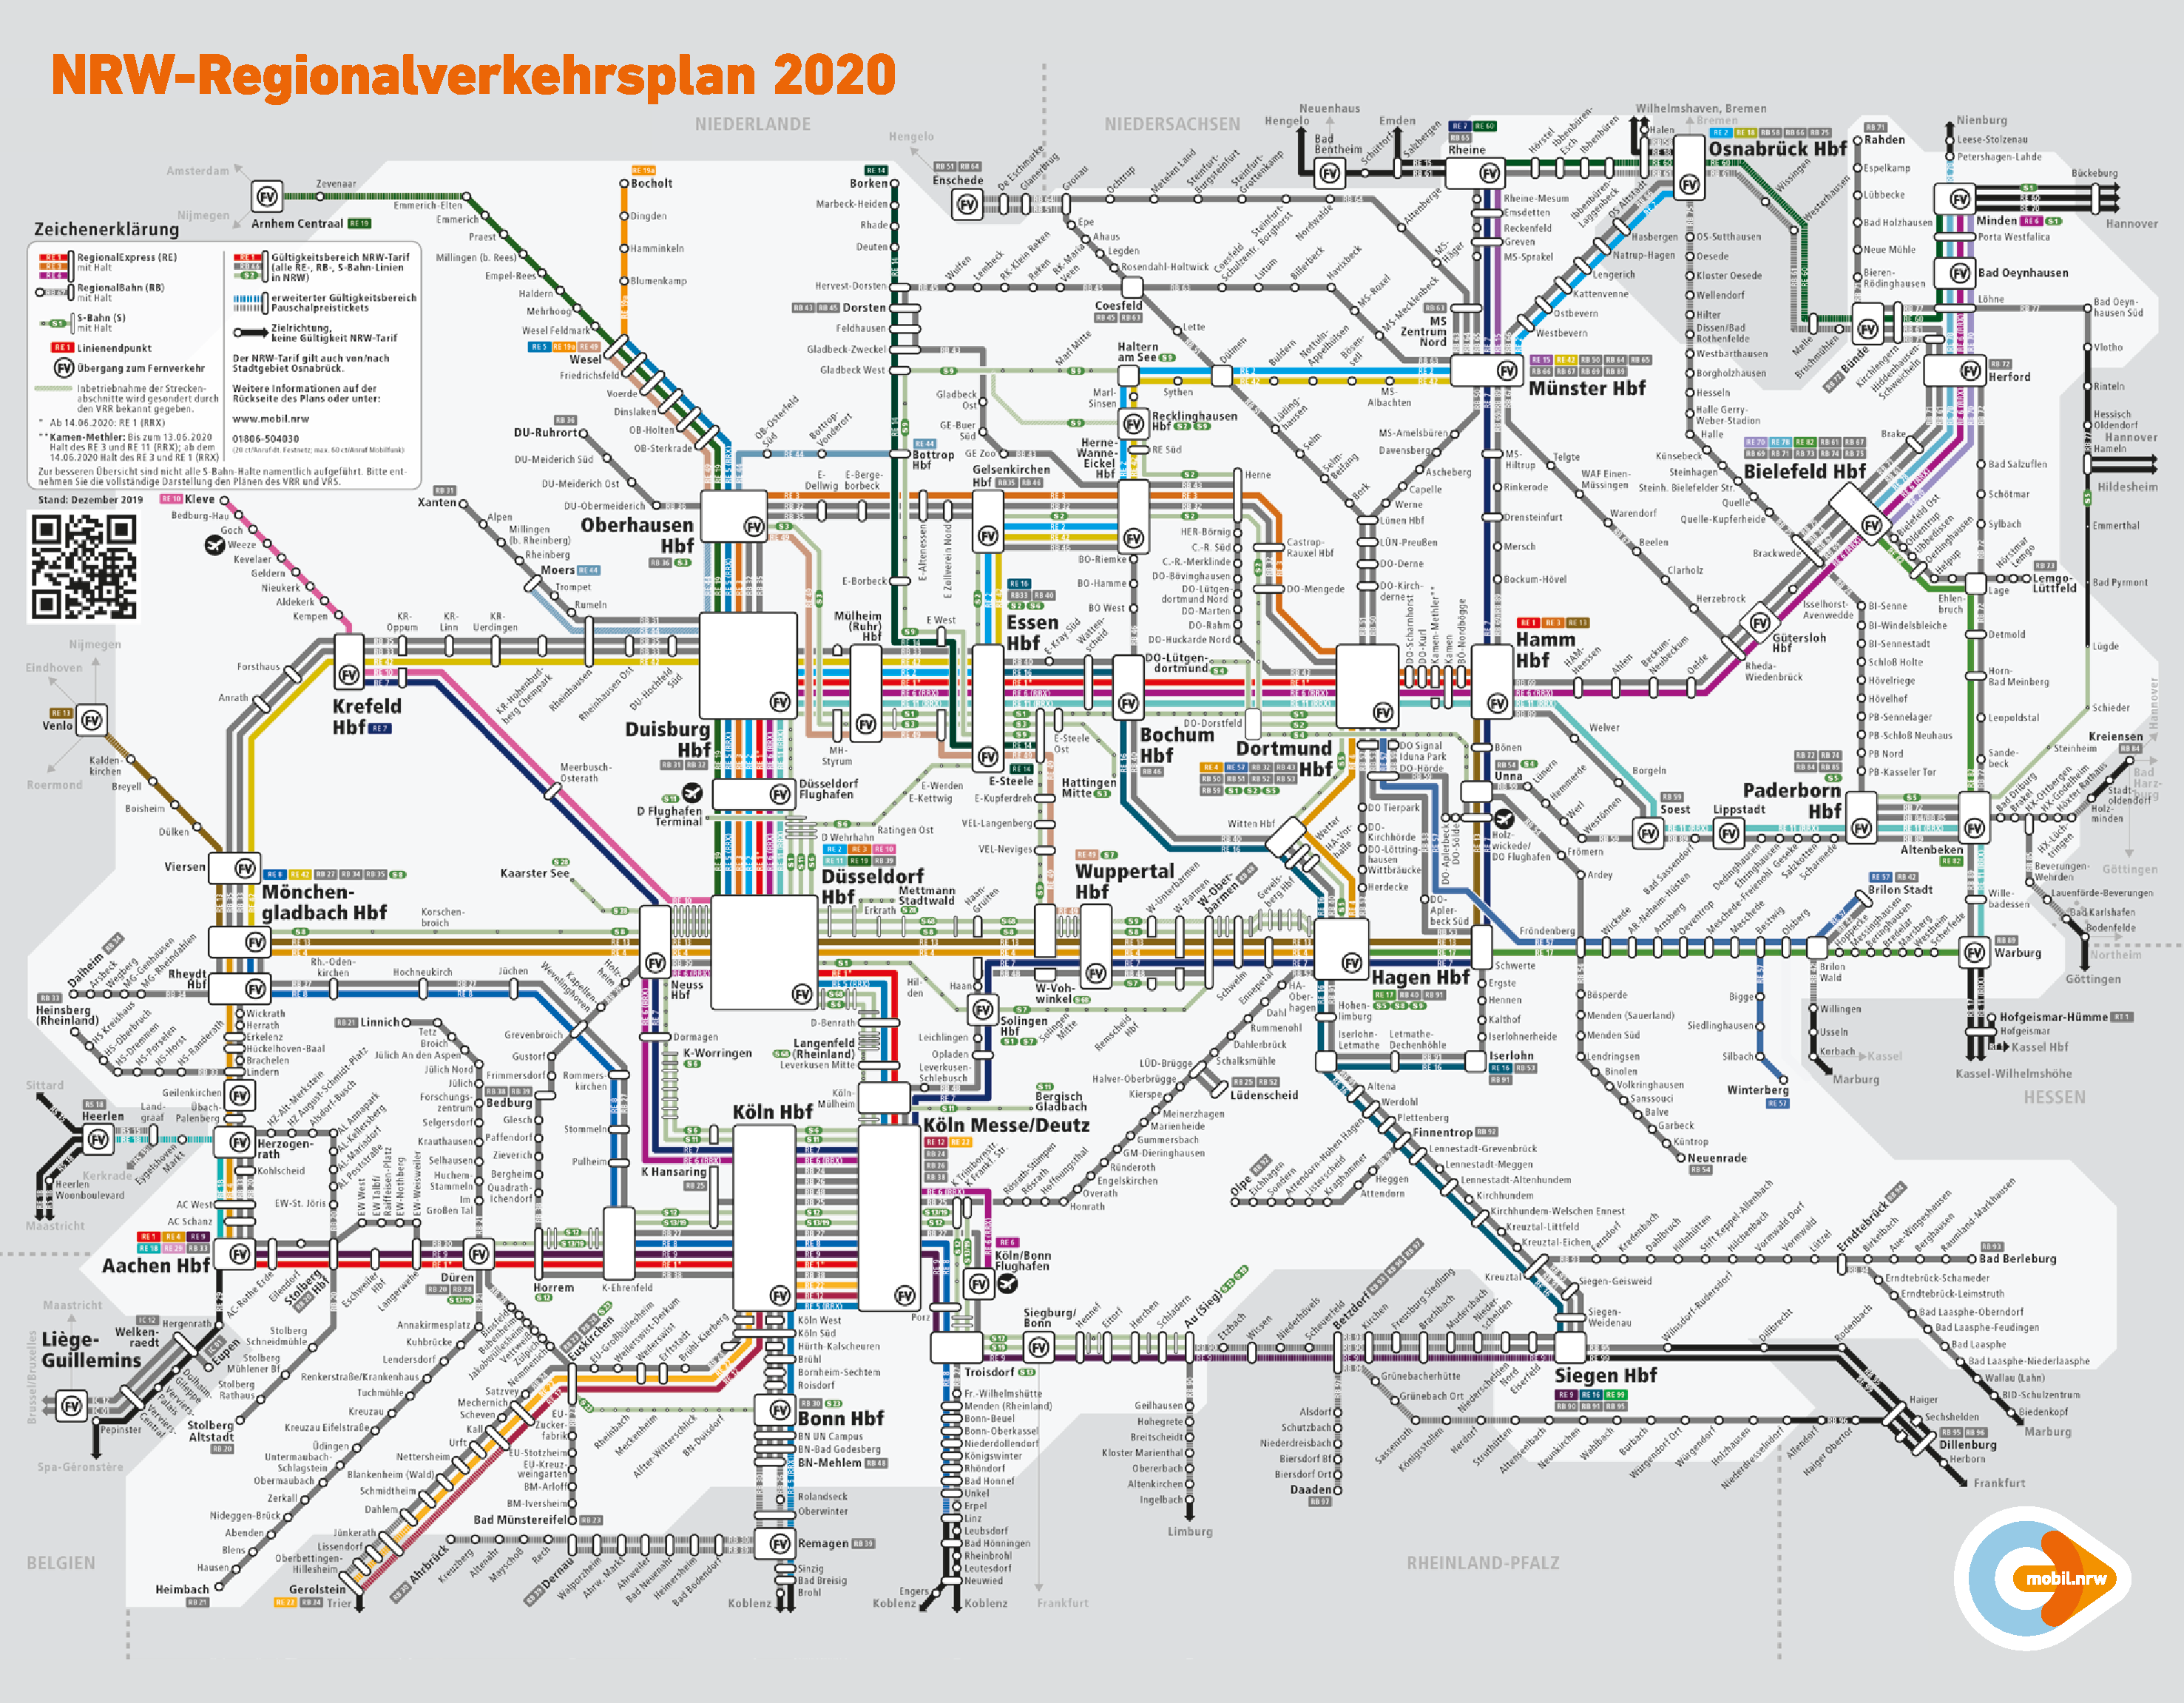
\includegraphics[width=\textwidth]{res/regionalverkehrsplan_nrw.pdf}
\end{figure*}
\textbf{Früher hab' ich mal geglaubt, das Semesterticket sei nur für den Weg nach Hause bestimmt, aber da lag ich nicht ganz richtig: Das Semesterticket~(SeTi) kann noch viel mehr.}

\includegraphics[width=\columnwidth]{res/semesterticket.pdf}

Vor Beginn jedes neuen Semesters bekommst du eine freundliche E-Mail, in der du dazu aufgefordert wirst, dich für das kommende Semester zurückzumelden. In dieser Mail ist auch ein Link zum SelfService-Portal enthalten, in dem du nach Bezahlen des Semesterbeitrags dein Semesterticket als PDF herunterladen kannst. Wir empfehlen außerdem das Ticket auszudrucken, falls der Handyakku doch einmal leer sein sollte.
Ohne einen gültigen Lichtbildausweis ist das Semesterticket nicht gültig.
Die meisten Busfahrer sehen es nicht als Verstoß an, wenn man mal keinen Lichtbildausweis bei sich trägt, doch spätestens, wenn du das Semesterticket für Fahrten mit der Bahn verwendest, musst du einen gültigen Ausweis bei dir tragen.

Der Universität Münster (bzw.\ dem AStA) ist es vor einigen Jahren nach langen Diskussionen und einer Urabstimmung gelungen, mit der Deutschen Bahn einen Vertrag über ein NRW-Ticket abzuschließen.
Daher darfst du dich im kompletten Nahverkehr in NRW bewegen.
Zusätzlich gilt das Ticket auch für ausgewählte Bahn-Strecken außerhalb von NRW, z.\,B.\ von Münster nach Osnabrück, Enschede (Niederlande) und Lingen oder auch von Lengerich (Westfahlen) nach Osnabrück (Details siehe Webseiten im "Ersti-Überlebenszettel" bzw.\ am Artikelende).

Nahverkehr bedeutet, dass du alle Busse, Straßenbahnen, U-Bahnen, S-Bahnen sowie alle Regionalbahnen -- RegionalExpress~(RE), RegionalBahn~(RB), und alle privaten Bahnen -- im Raum Nordrhein-Westfalen benutzen darfst.
Natürlich zählt der Fernverkehr -- InterCity~(IC) und InterCityExpress~(ICE) -- nicht zum Nahverkehr.

Solltest du mal mit der Bahn unterwegs sein und dein Semesterticket liegt zu Hause, ist das zwar ärgerlich, aber kein Beinbruch.
Zunächst wirst du vom Schaffner als "Schwarzfahrer" aufgeschrieben, mit dem Vorbehalt einer \SI{60}{\euro}-Strafe.
Dieses Schreiben musst du dann zusammen mit deinem Semesterticket am Schalter in Münster vorzeigen und musst nur eine Bearbeitungsgebühr in Höhe von ungefähr \SI{10}{\euro} bezahlen.
Ärgerlich, aber besser, als die ganzen \SI{60}{\euro} zu zahlen.

Solltest du mal per Anschlusszug über die Grenzen des NRW-/Semestertickets hinaus fahren wollen, denk daran, das nötige Ticket rechtzeitig (am besten gleich als "Viererticket") zu lösen, denn Nachlösen im Zug ist mittlerweile nicht mehr möglich.

Es ist von Zeit zu Zeit ganz ratsam, sich über die Optionen deines Semestertickets neu zu informieren.
So wurde zum Beispiel vor einiger Zeit geändert, dass du in Bussen \emph{im Stadtgebiet Münster sowie in Hamm, Rheine und Bocholt} ab 19~Uhr sowie an Wochenenden und Feiertagen ganztägig eine weitere Person oder ein Fahrrad mitnehmen darfst (gilt nicht für Bahnverbindungen).
Aufgrund des begrenzten Platzangebots kannst du dein Fahrrad allerdings nur mitnehmen, wenn die ausgewiesenen Stellflächen frei sind.
Auch neu ist, dass das Semesterticket für Erstsemester bereits einen Monat vor Semesterbeginn gilt. Wichtig dafür ist, dass du deine Studienbescheinigung ebenfalls ausgedruckt dabei hast.

\subsection{Das Kultursemesterticket}
Seit es 2015 durch eine Urabstimmung in der Studierendenschaft eingeführt wurde, gibt es neben dem Semesterticket das sogenannte Kultursemesterticket. Dieses wird ähnlich wie das Semesterticket aus den Semesterbeiträgen finanziert und erlaubt Studierenden, viele kulturelle Einrichtungen in Münster vergünstigt oder sogar kostenlos zu besuchen. Dies handelt der AStA jeweils direkt mit der ensprechenden Einrichtung aus – der Grad der Vergünstigung kann daher stark variieren. So bieten z.\,B. das Museum für Lackkunst und der Literaturverein freien Eintritt, während das Theater Münster ein festes Kontingent an Freikarten und kostenlose Restplätze anbietet und das GOP Variet\'e für einige Veranstaltungstermine jede Woche Sonderpreise für Studierende hat. Fußballfans dürfte interessieren, dass der AStA für jedes Heimspiel des SC Preußen Münster 50 Freikarten bekommt, die man sich beim AStA sichern kann.
Die vollständige Übersicht gibt es unter
\vspace{-1ex}
\begin{center}
	\url{https://www.asta.ms/kultursemesterticket}
\end{center}

\smallskip

\begin{center}
	\includegraphics[width=\columnwidth, height=0.12\textheight]{res/bushaltestelle.pdf}

	{\bfseries
	Aktualisierte Infos zum SeTi gibt es unter\\
	\url{https://www.asta.ms/semesterticket}}
	
	(weitere Links findet ihr im "Ersti-Überlebenszettel" auf Seite~\pageref{dpü} dieser Ersti-$\Phi$bel)
\end{center}

\fibelsig{Andreas G., Simon}
\end{multicols*}

\clearpage

% XXX Jedes Jahr Mensa-Preise prüfen!
\section[Das kleine Mensa~1~×~1]{\boldmath Das kleine Mensa~${1 \times 1}$}
\begin{multicols}{2}
\begin{quote}
	\textit{Allein zu essen ist für einen philosophierenden Gelehrten ungesund.}
	
	\hfill--- Immanuel Kant
\end{quote}

Alltäglich gegen Mittag beginnt der Magen zu knurren.
Für die Leute, die nicht jeden Tag selbst kochen wollen, am Nachmittag noch Veranstaltungen haben oder einfach soziale Kontakte pflegen wollen, gibt es die Mensa.
Das Gute ist, dass die Mensa~am~Ring direkt nebenan liegt.
Die meisten Studierenden gehen zwischen 11:45~Uhr und 12~Uhr direkt nach den Vorlesungen in die Mensa.
Dort erwartet euch dann meist eine lange Schlange, denn um 12~Uhr ist der Anlauf dort am größten. Wer dies umgehen möchte kann sich natürlich um 11:45~Uhr beeilen oder wenn möglich ein wenig warten. Um etwa 12:20~Uhr ist es meist schon wieder wesentlich leerer.
Doch auch die Zeit in der Schlange vergeht meistens recht schnell. Schwieriger ist da die Platzsuche, insbesondere für größere Gruppen. Gegen 12~Uhr ist die Mensa am vollsten, sodass mehr als 6 Personen Probleme bekommen können zusammen zu sitzen, danach leert sie sich langsam wieder. Um etwa 12:20~Uhr wird man kaum noch Sitzplatzprobleme haben.
Bevor man sich anstellt, ist es aber hilfreich, ein Bisschen über die Mensa zu wissen!

Seit dem Sommersemester 2017 benötigt man zum Bezahlen lediglich seinen Studierendenausweis.
Das Guthaben darauf kann an den Automaten im Foyer der Mensa und seit neuestem auch online aufgeladen werden.
Wenn das Guthaben nicht mehr ausreicht, um euer Essen zu bezahlen, könnt ihr den Ausweis auch an der Kasse noch aufladen. 
Das ist jedoch mit einem kleinen Aufpreis behaftet und euch ist die Missgunst an der Kasse und aller in der Schlange hinter euch sicher.
Falls ihr den Studierendenausweis noch nicht zugeschickt bekommen habt, könnte das daran liegen, dass ihr noch kein Foto dafür hochgeladen habt.
Das solltet ihr dann so bald wie möglich nachholen -- gerade, weil ihr diesen auch als Bibliotheksausweis und zum drucken und kopieren benötigt.

 \begin{center}
 	\includegraphics[width=.55\columnwidth]{private/res/studierendenausweis.pdf}
 \end{center}

Viel wichtiger aber stellt sich jeden Mittag erneut die Frage, was es überhaupt zu Essen gibt und was du selbst essen willst.
Dazu gibt es den Mensaplan, den ihr auf der Website der Mensa

\begin{center}
	(Link:
	\url{https://www.stw-muenster.de/de/essen-trinken/mensen/am_ring})
\end{center}

einsehen könnt. Dort könnt ihr den Plan entweder direkt im Browser öffnen (\url{https://muenster.my-mensa.de}) oder ihr ladet euch die zugehörige App herunter. Normalerweise geht man aber einfach los und schaut auf die
großen LCD-Bildschirme im Foyer. Dort könnt ihr alle Tagesangebote (z.\,B.\ auch die Beilagen und Desserts) sowohl "Oben" als auch im Buffetsaal "Unten" und deren Preise erfahren. Zusatzstoffe und Allergene werden unter den Gerichten mit Zahlen bzw. Buchstaben gekennzeichnet und andere eventuell wichtige Eigenschaften des Gerichts (z.\,B. "mit Schwein", "mit Fisch", "vegetarisch") werden mit Piktogrammen angezeigt. Die dazugehörige Legende hängt an verschiedenen Stellen bei Essensausgabe und Kassen oder kann unter den Tagesangeboten im Online-Mensaplan eingesehen werden.

Ein Blick auf die Angebote bevor ihr in der Schlange steht lohnt sich. Denn seit dem Sommersemester 2022 gibt es einige Änderungen im Preissystem, je nachdem wen man fragt mit Vorteilen und Nachteilen. Früher wurden "Oben" immer 4~Menüs mit jeweils drei beliebigen Beilagen zu festem Preis angeboten. Die Hauptgerichte der Menüs gibt es immer noch, wobei immer mindestens eine vegetarische und eine vegane Option dabei ist, die Beilagen müssen aber individuell zusammengestellt werden. Hier ist also meist Kopfrechnen gefragt, denn die Preise können ziemlich variieren. Jedes Hauptgericht und jede Beilage ist mit eindeutigem Preis auf dem Mensaplan gekennzeichnet. Das neue System sollte offiziell individuelle gerichte und transparente Preise ermöglichen, durch die Hintertür erfolgte dabei aber auch eine lange überfällige Preisanpassung.
Die Hauptgerichte liegen preislich nun bei \SI{1,10}{\euro} bis \SI{3,50}{\euro}. Hinzu kommen so viele Beilagen wie ihr möchtet bzw. euch leisten könnt. Zur Auswahl stehen meist Nudeln, Reis oder Kartoffeln, verschiedene Gemüseschälchen, Salate, Desserts, Obst und manchmal das Hauptgericht vom Vortag. Die Preisspanne reicht hier von \SI{0,30}{\euro} für Nudeln und Reis bis zu \SI{1,10}{\euro} für Salate und Desserts. Je nach Essensphilosophie können die Beilagen auf das Hauptgericht abgestimmt werden, aber auch Bratkartoffeln mit Pommes und Kartoffelbrei sind denkbar.

Nach einigen Mensabesuchen wirst du jedoch schnell bemerken, dass die Hauptgerichte sich alle paar Wochen wiederholen.
Das ist aber gar nicht so schlimm, denn die Gerichte schmecken dann wieder genauso gut oder schlecht wie zuvor.
Bei den ersten Besuchen solltet ihr aufpassen, dass die Bilder auf den Bildschirmen (soweit vorhanden) oftmals fast nichts mit dem Aussehen des Essens zu tun haben.

%\begin{center}
%	\fibelimgtext[bottom left]{
%		\includegraphics[width=0.95\columnwidth]{res/xkcd/149_sandwich.png}
%	}{\url{https://xkcd.com/149}}
%\end{center}

"Unten" im Buffetsaal gibt es ein vielfältiges Angebot von immer wiederkehrenden Menüs.
Jeden Tag könnt ihr an der Grillstation Currywurst mit Pommes oder ein Jägerschnitzel erwerben.
Regelmäßig gibt es den beliebten Mensaburger (auch vegetarisch) in verschiedenen Variationen, welcher so groß ist, dass sich an ihm die Geister scheiden, ob er mit Messer und Gabel oder mit der Hand gegessen werden muss.
An der Wokstation gibt es häufig Aktionen – meist aber Gerichte, die in großen Pfannen zubereitet werden können. Darunter vermutlich am wichtigsten ist das allseits beliebte (wirklich, die Schlange ist ein Alptraum) Gyros mit Tzatziki, viel Krautsalat und Pommes, das auch vegetarisch beliebt ist, dann aber ohne den Gyrosanteil und mit mehr Kraut.
Dazu gibt es eine Pastatheke, ein Buffet mit Nudeln, Aufläufen und aufgewärmten Resten (häufig eine Anlaufstelle wenn man sonst nichts mag) und ein Salatbuffet, an dem man sich auch Wraps zusammenstellen kann und das sich insbesondere im Sommer großer Beliebtheit erfreut. Allerdings eine Warnung: Die Teller vom Buffet werden an der Kasse nach Gewicht abgerechnet und das wird sehr schnell mehr als beim Zusammenstellen gedacht. Außerdem ist ein überquillender Wrap sein eigenes Problem.
Falls ihr Pommes nehmt, ist es empfohlen, mit Pommessalz nachzusalzen und gegen einen kleinen Aufpreis Majo oder Ketchup zu erstehen, Senf ist wie in einer richtigen Frittenbude kostenlos.
Des Weiteren gibt es fast immer einen sehr günstigen Eintopf an der passend genannten Eintopfstation.
Zu jedem Essen gibt es ein recht gutes Angebot an preiswerten Getränken.

Häufig gibt es (meist an der Wokstation) verschiedene Aktionen, so etwa in der jeweiligen Saison z.\,B. Spargelgerichte oder Erdbeeren mit Schlagsahne. Die Mensen achten dabei auch insgesamt auf Saisonalität und Regionalität in den Gerichten, so stammen zum Beispiel die Kartoffeln ausschließlich aus dem Münsterland.
%Seit Neuerem bietet die Mensa außerdem regelmäßig Friedensteller an. Dies sind Gerichte, die nach Rezepten der Friedensteller-Intiative (überraschend, ich weiß) gekocht wurden und sich durch Nachhaltigkeit auszeichnen, z.\,B. durch Saisonalität und Regionalität der Zutaten. Diese ersetzen normalerweise eine vegetarische (oder in einigen Fällen vegane) Auswahl "Oben".

Wenn ihr fertig mit dem Essen seid, seid ihr noch lange nicht mit der Mensa fertig!
Entweder ihr holt euch noch einen Nachschlag oder ihr macht euch mit eurem Tablett auf zum Geschirrband und der meist etwas murrig schauenden Person dort.
An der Wand hängt dann eine genaue Anleitung, wie ihr euer Geschirr zu sortieren habt, damit es keinen Ärger vom Mensapersonal gibt.

\fibelimgtext{
	\includegraphics[width=\columnwidth]{res/xkcd/720_recipes.png}
}{\url{https://xkcd.com/720}}

Falls jedoch jemand gar nichts gefunden haben sollte, kann man es auch mit einer Pizza oder einer Waffel im Viva Campus-Café im Erdgeschoss versuchen.
Hier werden auch die meisten anstehenden Sportereignisse übertragen und morgens in der Wiederholung gezeigt.
Außerdem kann man hier recht entspannt sitzen und etwa eine Kaffeespezialität trinken.

Dazu kommen noch diverse Läden wie ein sehr nützlicher Copyshop und Schreibwarenladen (Kopieren und Drucken ist allerdings preiswerter, wenn man Print~\&~Pay beim ZIV nutzt oder mit dem Guthaben des Studierendenausweis an den Kopierern z.\,B.\ im Lernzentrum, der IG1 oder im ZIV. Aber vergesst eure Karte dort nicht!). Außerdem gibt es noch eine Filiale der Techniker Krankenkasse, den Aster Reise Service, einen Info-Point des Studierendenwerks und zwei Geldautomaten.

Alternativ könnt ihr auch die anderen Mensen in Münster besuchen, insbesondere die größte, die Mensa~am~Aasee, sei hier aufgrund der großen Auswahl an Salaten und dem grandiosen Buffet empfohlen. Nebenan gibt es zudem das Café Hier und Jetzt, welches rein vegetarische und vegane Gerichte anbietet und sogar Abends und Samstags geöffnet ist. Die anderen Mensen und Cafés findet ihr auch alle in der Mensa-App.

\fibelsig{Moritz}
\end{multicols}

\clearpage

\section{Internet, IVV~NWZ, Computer\-Labs~\&~Co.}
\begin{multicols*}{2}
	\fibelimgtext[below left]{
		\includegraphics[width=\columnwidth]{private/res/comics/hacker.pdf}
	}{Jan Tomaschoff\qquad© Cartoon-Caricature-Contors, Pfaffenhofen}
\subsection{WLAN für alle!}
Wo mittlerweile viele Restaurants und Cafés freien Internetzugang über WLAN zur Verfügung stellen und Politiker damit werben, das an Münsteraner Schulen fortzuführen, in einer Zeit, in der wissenschaftliches Arbeiten ohne den schnellen Austausch relativ großer Daten nicht mehr denkbar ist, gibt es natürlich auch an der Universität eures Vertrauens frei verfügbaren WLAN-Zugang für jeden. Solange er Mitarbeiter oder Student der WWU oder einer am eduroam-Projekt teilnehmenden Hochschule ist.
Außerdem bekommt ihr noch ein ganzes Paket an Cloud-Speichern und könnt im Uni-Netz sogar von überall aus drucken oder eigentlich teure Bücher und Programme herunterladen.

\subsubsection{Und wie funktioniert das?}
Ihr erhaltet bereits mit eurer Einschreibung in die Uni eine Nutzerkennung der Form \texttt{v\_nnnn\#\#} mit zugehörigem Passwort, die aus eurem Vor- und Nachnamen sowie zwei Zahlen gebildet wird -- für "Max Mustermann" wäre eine mögliche Kennung "\texttt{m\_must08}".
Zusätzlich erhaltet ihr eine Uni-E-Mail-Adresse -- hängt für diese einfach \texttt{@uni-muenster.de} oder \texttt{@wwu.de} (funktioniert beides) an eure Nutzerkennung an.

Wie viel seine Nutzerkennung kann, hängt von den Nutzergruppen ab, die der Kennung zugeordnet ist. Für Studierende der Physik sind das zunächst \texttt{u0dawin} (Studierende) und \texttt{p0stud} (Angehörige der Physik). Ansich braucht ihr euch darum nicht wirklich kümmern -- wenn ihr neue Rechte braucht, werden euch die entsprechenden Nutzergruppen zugeordnet.

Kurzgesagt: Ihr habt automatisch, da ihr Physik an der WWU studiert, eine Reihe toller, kostenloser Angebote, die ihr mit eurer Nutzerkennung nutzen könnt.

\subsection{Was kann man denn nun alles machen?}
So einiges. Der wichtigste Dienst ist dabei wohl euer E-Mail-Postfach.
Viele relevanten Infos werden euch darüber geschickt -- So zum Beispiel die Aufforderung, den Semesterbeitrag zu zahlen, oder die Information, dass eine Vorlesung kurzfristig ausfällt.
Ihr seid sogar verpflichtet, die Mails der Universität zu lesen -- Wenn ihr also den Semesterbeitrag nicht zahlt, werdet ihr sogar exmatrikuliert -- also passt auf! Auch die Erinnerung zur Prüfungsanmeldung und unseren Newsletter sowie Infomails (mit denen wir uns aber sehr zurückhalten, wir wollen euch ja nicht "zuspammen", und auch wir kennen das Problem überfluteter Postfächer :) ) erhaltet ihr per Mail an eure Uni-Adresse.

Uns, die Fachschaft eures Vertrauens, erreicht ihr übrigens über die Adresse \email{fsphys@uni-muenster.de}.

\subsubsection{Portale}
Im Portal myWWU (\url{https://www.uni-muenster.de/mywwu}) sind die wichtigsten Dienste der Uni zusammengefasst.
Dazu gehören insbesondere das E-Mail-Postfach und das Vorlesungsverzeichnis (HIS~LSF) es gibt aber auch einen Kalender (der euch auch erinnert, wann ihr Bücher zurückgeben müsst) und von euch ausgewähle Newsfeeds\dots Wenn man myWWU richtig nutzt, kann es sehr praktisch sein.

Auch sehr nützlich ist der Zugriff auf disco (\url{https://disco.uni-muenster.de}), das Suchsystem der ULB.
Hier sind der OPAC (ein Katalog- und Ausleihsystem der ULB) und viele weitere Verzeichnisse integriert, sodass ihr in vielen Millionen Dokumenten suchen könnt.
Ihr braucht also nicht jedes Mal zur ULB zu laufen, um Bücher zu verlängern.
Wesentlich wichtiger sind jedoch Buch- und Literaturrecherchen, die ihr schnell und effektiv per Netz an den verschiedensten Stellen machen könnt.
Daneben gibt es über die ULB und den Fachbereich Physik auch einen kostenlosen Zugang zu allen wesentlichen wissenschaftlichen Zeitschriften und zu vielen Bücher z.\,B.\ von Springer.

Ruft dazu aus dem Uni-Netz (welches ihr auch von zu Hause aus über das sogenannte VPN der Uni erreicht) die Webseite \url{https://link.springer.com} auf und ladet das Buch eurer Wahl einfach herunter.

\begin{center}
	\includegraphics[width=\columnwidth, height=0.3\textheight]{private/res/comics/computersuechtig.pdf}
\end{center}

\subsubsection[Sichere Datencloud -- sciebo!]{Sichere Datencloud -- sciebo! \cref{internet:sciebo}}
Seit Kurzem bietet die WWU gemeinsam mit anderen nordrhein-westfälischen Hochschulen eine Dropbox-ähnliche Cloud an, die im Gegensatz zu anderen bekannten Online-Speicherdiensten betont nicht-kommerziell ist und viel Wert auf Datenschutz legt.
Ganz abgesehen davon, dass die Idee zur Cloud von einem Fachschaftler kam -- Danke, Markus :) -- ist Sciebo auch wegen seiner guten Umsetzung und einfacher Bedienoberfläche unbedingt empfehlenswert.
Einfach auf \url{https://www.sciebo.de} registrieren und dann mit \texttt{<nutzerkennung>@uni-muenster.de} als Benutzername und dem soeben gewählten Passwort anmelden.
Insgesamt bekommt man dort \SI{30}{\giga\byte} freien Speicherplatz, auf den man von überall aus über's Internet Zugriff hat.

\subsubsection{Spielregeln}
Ihr habt einen ungefilterten, schnellen Zugang zum Internet und damit Zugriff auf alle möglichen Angebote.
Es sollte daher nicht unerwähnt bleiben, dass trotz der großen Zahl an Mitgliedern der Uni zurückverfolgt werden kann, wer Urheberrechtsverstöße und andere illegale Aktivitäten durchführt.
Ebenfalls führt z.\,B.\ der Versand von Spam und Viren zu einer Sperrung des Netzzugangs -- Die Sanktionen bei Zuwiderhandlung sind in der Benutzungsordnung geregelt.
Dies soll euch nicht abschrecken, dennoch solltet ihr die Spielregeln kennen.

\subsubsection{ComputerLabs}
An quasi jedem Rechner der WWU habt ihr Zugriff auf euer persönliches Benutzerkonto -- Einfach Nutzerkennung und Passwort eingeben und los geht's.
Der Fachbereich Physik hat, auf mehrere Gebäude verteilt, "ComputerLabs" eingerichtet, an denen eine große Zahl an Rechnern für euch zur Verfügung stehen.
Mit eurer Nutzerkennung könnt ihr übrigens auch die Rechner in den Labs der Biologie und Chemie benutzen -- und umgekehrt.
Dass ihr überall dieselbe Arbeitsumgebung, euer Netzlaufwerk (Laufwerk \texttt{I:} mit \SI{10}{\giga\byte} Speicherplatz) und die gleichen Programme vorfindet, dafür ist gesorgt.
Außerdem gibt es noch allgemein zugängliche ComputerLabs wie die im ZIV~(Einsteinstraße~60).
Diese können von allen Angehörigen der Uni verwendet werden, allerdings stehen euch hier nicht dieselbe Software-Auswahl und Arbeitsumgebung zur Verfügung wie bei den Rechnern des naturwissenschaftlichen Zentrums.
Standardmäßig ist beispielsweise nur euer ZIV-Netzlaufwerk (Laufwerk \texttt{U:} mit \SI{4}{\giga\byte} Speicherplatz) und nicht das \texttt{I}-Laufwerk eingebunden.

Die ComputerLabs der Physik findet ihr an folgenden Orten:
\begin{description}
	\item[Angewandte Physik:] 10~Windows-PCs.
	\item[Lernzentrum:] 6 PCs
	\item[Institut~für~Kernphysik,] 2.~Stock: 11~Windows-PCs, Scanner, s/w-Laserdrucker.
	\item[Institut~für~Theoretische~Physik,] 4.~Stock: 11 Windows-PCs.
	\item[Institutsgruppe~1~(IG1):]~
		\begin{itemize}[leftmargin=1mm]
			\item StudiBib, Erdgeschoss, Raum~13: Zwei Windows-PCs, Scanner, Farbdrucker.
			\item Institut für Technik und ihre Didaktik (Raum 220): 9~Windows-PCs, s/w-Laserdrucker.
			\item Physikalisches~Institut, 5.~Stock, Räume~504 und 520: insgesamt 9~Windows-PCs, A3-Flachbettscanner, s/w- und Farblaserdrucker.
			\item Institut~für~Festkörpertheorie, Raum~745 und 747: insgesamt 21~Windows-PCs, Scanner, s/w-Laserdrucker.
		\end{itemize}
	\item[Institut~für~Geophysik,] Corrensstr., Raum~301 und 333, je 10~Windows-PCs.
	\item[Seminar für Didaktik des Sachunterrichts]~\\(DDSU) im Leonardo-Campus~11, Raum~104: 9~Windows-PCs, s/w-Laserdrucker.
\end{description}

Die jeweiligen Ansprechpartner für Fragen, Probleme und auftretenden Fehler sind im jeweiligen ComputerLab bekanntgegeben.
Auf all diesen Computern ist ein sehr umfangreiches Software-Angebot installiert, sodass ihr dort direkt arbeiten könnt.
Eine Übersicht gibt es auf der Internetseite der IVV~NWZ~\cref{internet:ivvnwz}.

Der Begriff "IVV" stammt übrigens daher, dass es neben dem ZIV -- für die zentrale Bereitstellung von IT an der Uni zuständig -- an der Uni zehn sogenannte dezentrale "Informations-Verarbeitungs-Versorgungseinheiten" (IVV) gibt, die für bestimmte Bereiche zuständig sind.
Für die Fachbereiche Biologie, Chemie und Physik ist das die IVV~NWZ (IVV~4).

\fibelimgtext[bottom left]{
	\includegraphics[width=\columnwidth]{res/xkcd/722_computer_problems.png}
}{\url{https://xkcd.com/722}}

\subsubsection[Weitere Angebote der IVV~NWZ und des ZIV]{Weitere Angebote der\\IVV~NWZ und des ZIV}
Sowohl die IVV~NWZ (mit "nwzcitrix" via Uni-VPN) als auch das ZIV (mit "rd.wwu.de") betreiben Remote-Desktop-Server, auf die ihr von Zuhause aus zugreifen könnt.
Damit habt ihr auch von Zuhause aus Zugriff auf die meiste Software und könnt damit arbeiten.
Das Stichwort "Cloud" fällt meist irgendwann in diesem Zusammenhang und sollte heutzutage jedem bekannt sein.
Etwas Ähnliches bieten IVV und ZIV schon seit vielen Jahren allen Studierenden an.
Bei der IVV gibt es \SI{10}{\giga\byte} Speicherplatz (Laufwerk~\texttt{I:}) und beim ZIV \SI{4}{\giga\byte} (Laufwerk~\texttt{U:}), s.~oben.
Dieser Speicherplatz kann auch ähnlich wie eine Festplatte auch Zuhause angebunden werden.

Auch kostengünstige Druckmöglichkeiten (A4 bis A0, auch in Farbe) werden angeboten; für die Nutzung ist eine kostenlose Anmeldung bei "Print~\&~Pay" (in MeinZIV; Link im Abschnitt~"Der Ersti-Überlebenszettel", S.~\pageref{dpü} in dieser Fibel) erforderlich.
Weitere Informationen hierzu und vielen weiteren Angeboten sowie Anleitungen gibt es bei der IVV~NWZ~\cref{internet:ivvnwz} und beim ZIV~\cref{internet:ziv}, sowie in der Ersti-Woche und bei uns~\cref{internet:fsphys_software}.

\subsubsection{Software für Zuhause}
Für Studierende gibt es beim ZIV zwei interessante Softwarepakete, die insbesondere auch für den privaten Einsatz auf den eigenen Computern vorgesehen sind.
Interessant ist vor allem die Anti-Virus-Software (Sophos), welche von der Uni für alle bezahlt wird.
Zusätzlich können viele weitere Programme, die das ZIV betreut, auch auf dem eigenen Rechner installiert und unter einigen Bedingungen genutzt werden~\cref{internet:ziv_software}.

Die IVV~NWZ ermöglicht zudem allen zugehörigen Studierenden den Zugriff auf das Imagine-Programm von Microsoft.
Damit habt ihr Zugriff auf fast die gesamte Software-Palette von Microsoft, ausgeschlossen sind nur einige Office-Programme wie Word, Excel und PowerPoint.
Diese Software dürft ihr ausdrücklich auch auf privaten Rechner installieren.
Weitere Programme wie die Mathematik-Software "Mathematica" (vielen vielleicht bereits durch die -- übrigens fürs Studium häufig nützliche -- Webseite WolframAlpha \cref{internet:wolfram_alpha} bekannt) können ebenfalls unter verschiedenen Bedingungen bezogen werden -- Mathematica kann beispielsweise nur im Uni-Netzwerk (d.\,h.\ zum Beispiel von Zuhause über eine VPN-Verbindung) genutzt werden.
Weitere Infos findet ihr wieder unter \cref{internet:ivvnwz}, \cref{internet:ziv} und \cref{internet:fsphys_software}.

\subsection{Links}
\begin{flushleft}
	\begin{fibelurl}
		\url{https://www.sciebo.de}
		\label{internet:sciebo}
	\end{fibelurl}
	\begin{fibelurl}
		\url{https://www.uni-muenster.de/NWZ}
		\label{internet:ivvnwz}
	\end{fibelurl}
	\begin{fibelurl}
		\url{https://www.uni-muenster.de/ZIV}
		\label{internet:ziv}
	\end{fibelurl}
	\begin{fibelurl}
		\url{https://www.uni-muenster.de/Physik.FSPHYS/service/software}
		\label{internet:fsphys_software}
	\end{fibelurl}
	\begin{fibelurl}
		\url{https://www.uni-muenster.de/ZIV/Software/Uebersicht.html}
		\label{internet:ziv_software}
	\end{fibelurl}
	\begin{fibelurl}
		\url{https://www.wolframalpha.com}
		\label{internet:wolfram_alpha}
	\end{fibelurl}
\end{flushleft}

\fibelsig{Simon, Benedikt}

\medskip

\begin{center}
	\fibelimgtext[below right]{
		\includegraphics[width=\columnwidth, height=0.2\textheight]{res/xkcd/327_exploits_of_a_mom.png}
	}{\url{https://xkcd.com/327}}
\end{center}
\end{multicols*}


\clearpage

\section[Gruß von der anderen Seite (ein ehemaliger Physikstudent erzählt \dots)]{Gruß von der anderen Seite\\(ein ehemaliger Physikstudent erzählt \dots)}
\textbf{
Ja, es gibt ein Leben nach dem Physikstudium, auch wenn viele von euch sich das aktuell sicher noch nicht vorstellen können.
In diesem Erfahrungsbericht könnt ihr einen kurzen Einblick in das (Studien-)Leben von Philipp werfen, der bis vor knapp zwei Jahren selber noch Physikstudent (1-Fach-Bachelor) hier in Münster war.
}


\begin{multicols}{2}

\begin{wrapfigure}[11]{r}{0cm}
	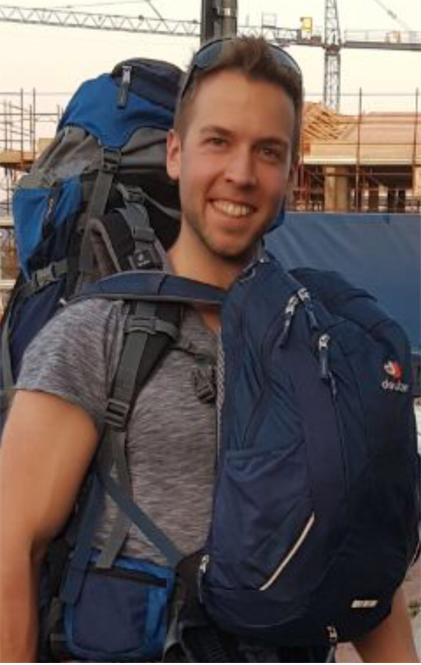
\includegraphics[width=3.2cm]{res/philipp_van_wickevoort_crommelin.PNG}
\end{wrapfigure}

"Was machst Du eigentlich nach dem Abi?", unterbrach ich das abwechslungslose Rauschen des 70\,PS schwachen Dieselmotors unseres
VW-Bus-T3s bei 80\,km/h Höchstgeschwindigkeit auf der slowenischen Avtocesta, der Bundesautobahn A2, bei der Durchfahrt im
Karawankentunnel – noch rund 300\,km von unserem Ziel, der kroatischen Halbinsel Istrien, entfernt.
Mich verblüfft heute noch, wie prompt die Antwort kam.

"Physik studieren!", erwiderte mein guter alter Freund Johann und fügte nach kurzer Pause hinzu:
"Weil ich dort die Fähigkeit erlerne, logisch zu denken."
Das Selbstverständnis, das in der Betonung seiner Antwort lag, sollte noch viele Jahre in meinem Bewusstsein wiederhallen... \\ 

Rund ein Jahr später besiegelte ich meine schulische Laufbahn mit einem durchschnittlichen bis guten Abitur und entschied daraufhin,
eine Rucksackreise nach Zentralamerika anzutreten.
Dort hatte ich vor allem eines: Zeit. In erster Linie habe ich die dazu genutzt, um meine Reise mit jedem Schritt zu genießen.
Es gab allerdings auch ausreichend Zeit, um etwas mehr über die nächsten, größeren Schritte im Leben zu sinnieren. Johanns Bemerkung fiel mir wieder in den Sinn... \\ 

Physik studieren? Das ist doch nur was für hochbegabte Nerds, für Außenseiter, die sich während der Schulzeit regelmäßig zu LAN-Parties verabredeten und 
von den \textit{coolen} Jungs kopfüber in die Kloschüssel getaucht wurden -- ein Auffangbecken der personifizierten, sozialen Inkompetenz.
Zu dieser Sorte Jungs habe ich zwar nie gehört, allerdings auch nicht zu den Überfliegern.
"Physik ist die Mutter aller Naturwissenschaften!", erinnerte ich mich an das – zumindest im monatlichen Intervall – gebetsartig aufgesagte Mantra unseres
Physik- und Klassenlehrers. Je mehr ich darüber nachdachte, desto mehr klang es nach Herausforderung,
nach einem Tiefentauchgang in die Welt der Astronomie und der Quanten.
Es klang nach Aussicht auf ein tiefgreifendes Verständnis der uns umgebenden Welt. Ich wollte es versuchen... \\ 

Beim Besuch der ersten Mathe-\textsc{I}-Vorlesung an der \textsc{Christian-Albrechts}-Universität zu Kiel ahnte ich nichts von meinem Glück, dass mir dieses Fach in den kommenden Monaten 90\,\% meiner Kopfschmerzen
verursachen und zeitlichen Kapazitäten abverlangen würde.
Auf die restlichen 10\,\% fielen Physik \textsc{I}, ein Computer-, ein Chemie- und ein weiterer – allerdings etwas angewandterer – Mathe-Grundkurs. \\ 

Ich wollte ihn schon korrigieren... Der Professor musste dem Anschein nach völlig falsch verstanden haben, was \textit{Mathematik} eigentlich war,
nämlich eine Gleichung nach $x$ umzustellen oder mal eine Kurvendiskussion durchzuführen – so hatte man es doch noch aus der Schulzeit in Erinnerung.
Anstelle dessen wurden Axiome, Lemmata, Beweise, Abschätzungen und Grenzgänge allgegenwärtiges Idiom.
Man musste schon aufpassen im privaten Umfeld zu vermeiden, jeden Satz mit "Sei Epsilon größer Null..." anzufangen. \\ 

Ich habe gebüffelt wie verrückt und nach Abschluss der Matheprüfung mit Note 3,7 wurden mir zwei Dinge klar: 1., das Physikstudium ist undankbar aber
machbar – auch als Normalo – und 2., die Regelstudienzeit ist definitiv keine Option - jedenfalls nicht als Normalo.
So wurden aus 6 Semestern 1-Fach-Bachelorstudium am Ende 8, womit für ein Studentenleben außerhalb des
Bibliothekskellers endliche Wahrscheinlichkeiten bestanden. Nach diesen 8 Semestern hatte ich 1., einen 1-Fach-Bachelor der Physik, 2., ein paar Tassen weniger im
Schrank und 3., die Faxen von der Materie erstmal dicke. \\ 

Zur Frage nach dem \textit{nächsten Schritt} war man gar nicht gekommen und plötzlich sah man sich damit konfrontiert.
Wer sich diese Frage stellt, kommt allerdings gleich zur nächsten: "Was, zur Hölle, will ich mit einem Abschluss in Physik?". \\ 

Ich wusste jedenfalls, falls es weitergehen soll, dann musste ein Tapetenwechsel her – andere Stadt, andere Uni, andere Professoren und andere Themen.
Nach einiger Recherche habe ich mich für Münster entschieden – Deutschlands Fahrradhauptstadt.
Das war eine gute Idee, denn in Münster gibt es scheinbar keine Probleme: 

Hoppelnde Karnickel auf Hauptverkehrskreiseln, perfekt begradigte Straßenmarkierungen auf perfekt geteerten Straßen, eine Polizei, die systemgefährdende Über-Rot-Gänger noch zur Rechenschaft zieht, die perfekte Balance zwischen städtischem Erholungs- und Wohnraum, kulturelle Vielseitigkeit für Jung und Alt und ein gefühlt verpflichtender, allsonntäglicher Kirchengang, den erfolgreich zu vermeiden sicherlich kein Problem darstellen würde. Kurzum, Münster war das perfekte Umfeld für ein akademisches Aufbaustudium unter Vermeidung blasphemischer Ablenkungen. \\ 

Wer das Masterstudium dann beginnt, kann sich erstmal zurücklehnen.
Die Vorlesungen können meist aus einem sehr vielfältigen und stark individualisierbaren Studienprogramm zusammengestellt werden. 
Die Tage der großen Vorlesungshörsäle sind gezählt und man sitzt meist nur noch mit wenigen Kommilitonen zusammen und pflegt ein wesentlich
persönlicheres Verhältnis zum Professor.
Wer sich für ein Masterstudium der Physik entscheidet, der beweist nicht zuletzt seine Überzeugung, die er der Sache widmet.
Die Probezeit ist sozusagen vorbei und dieses Gefühl wird einem meist auch von den Dozenten widergespiegelt. \\ 

Die Frage, was ich mit einem Master-Abschluss der Physik eigentlich machen will, war immer noch ungeklärt und so entschied ich mich für ein Praktikum in einer Bank.
Wie ich darauf kam? In Münster kann man sich so ziemlich alles in den Studienplan laden,
so auch das Seminar \textit{Finanzmathematik und Risikomanagement} des theoretischen Kernphysikers \textsc{Dr. Jörg C. Lemm}, das dem Alltag erfrischend abwechslungsreichen Kontrast verpasste. \\ 

Ich kann jedem ein Praktikum nur empfehlen. Nicht zuletzt, weil man als Physikstudent häufig wenig Vorstellung davon hat, was man außerhalb der Uni alles tolles mit seinem Wissen anfangen kann.
Ich fand die Bankenwelt interessant, insbesondere, weil man dort die erlernte Mathematik und erlernten Programmierkenntnisse einbringen konnte.
Heute arbeite ich für die parcIT GmbH, dem "Partner für Risikomanagement und Controlling".
Meine Arbeit macht mir Spass, ich kann viel programmieren, knifflige Probleme kreativ lösen und habe tolle Kollegen. Warum ich nach meinem Master-Abschluss keine Promotion machen wollte?
Vielleicht kommt die irgendwann noch mal. Lebensläufe sind heutzutage nichtlinear und solche Möglichkeiten bleiben meiner Ansicht nach weiter offen. \\ 

Zum Schluss zurück zu Johanns Aussage. Erlernt man im Physikstudium die Fähigkeit logisch zu denken? Ich denke mittlerweile,
dass ein rationaler Denkapparat eine durchaus gewinnbringende Komponente in der Ausbildung zum Physiker ist. Es geht aber vielmehr darum,
das Handwerkszeug an die Hand zu bekommen, ein komplexes Problem in einfachere, verdaulichere Bausteine zu zerteilen,
die mit mathematischer Logik und den Gesetzen der Natur gelöst werden können.
Es sollte einem klar sein, dass man im Gegensatz zu einem Ingenieur oder einem Architekten keine spezifische Berufsausbildung genießt.
Als Physiker ist man Generalist, der allerdings dazu befähigt ist, sich in jede erdenklich Nische einzuarbeiten und sich auf diese zu spezialisieren. \\ 

Deswegen lautet mein Appell an alle, die noch an der Entscheidung zweifeln: "Traut Euch, denn es lohnt sich!" und alle, die unter dem Druck des Studiums leiden: "Haltet durch, denn es lohnt sich!" Ich für meinen Fall, würde es wieder machen. \\ 

\vspace{0.8cm}

\textsc{Philipp van Wickevoort Crommelin}  



\end{multicols}

\clearpage

\section[Die Fachschaft]{Die Fachschaft -- Unsere Selbsthilfegruppe}
\label{fsphys:sec}
\begin{center}
	\vspace{-0.5cm}
	\includegraphics[width=0.7\textwidth]{res/fsphys_logo.pdf}
	\vspace{-0.5cm}
\end{center}
\begin{multicols}{2}
% \subsection in diesem Artikel kleiner (mit \normalsize) darstellen,
% sonst ist zu wenig Platz
\addtokomafont{subsection}{\normalsize}
% etwas weniger Platz vor/nach \subsection (wie bei \subsubsection), sonst ist
% immer noch zu wenig Platz
\fibelspacingsubsubsection[subsection]

\textbf{Fragst du dich mittlerweile, wer eigentlich allen Leuten hilft, das Studium zu überstehen? Fragen zu beantworten, für Klausuren zu lernen und so das Studium zu meistern?}

Willkommen bei der Fachschaft.
"Fachschaft" -- das Wort wirst du schon ab und zu gehört haben.
Die Webseite, auf der du einen ersten Stundenplan bekommen und Informationen zur Ersti-Woche gefunden hast, trug das Wort im Namen\dots

\subsection*{Aber wer ist überhaupt "die Fachschaft"? Und was macht die eigentlich?}
"Die Fachschaft" ist eigentlich ein bisschen ungenau.
Eigentlich heißen wir "Fachschaftsrat Physik" und bei uns machen die Studierenden mit, die Spaß daran haben, anderen ehrenamtlich zu helfen und sich dabei untereinander auszutauschen.
Wenn man in der Fachschaft aktiv ist, hat man zwar zeitweise ein bisschen mehr zu tun, lernt aber dafür eine ganze Reihe neuer Leute gleicher Gesinnung kennen.

Einen Teil unseres Angebotes nutzt du jetzt gerade.
Ja, in diesem Moment.
Das Stück Papier, das du gerade in den Händen hältst (oder die Datei, die du gerade liest), haben wir für dich gebastelt -- mit der Gewissheit, einer ganzen Reihe an Erstsemestern weiterzuhelfen.

Und vermutlich hast du auch an der "Ersti-Woche" bzw.\ "O-Woche" teilgenommen und hoffentlich wertvolle Informationen für den Studienbeginn gesammelt.

\subsection*{Klausuren und Prüfungen meistern}
Zu unserem Angebot gehört aber auch das Verleihen von (digitalen) Alt-/Musterklausuren und Prüfungsprotokollen.
Das funktioniert, weil Studierende (also am besten auch ihr!) und Professoren uns Fotos oder Digitalversionen davon vorbeibringen und ihr Protokolle eurer mündlichen Prüfungen zur Verfügung stellt, sobald ihr welche habt.
Durch eure Mithilfe bekommt ihr so die Gewissheit, den nachfolgenden Generationen von Studierenden in der "Schlacht" mit dem Physikstudium etwas weitergeholfen zu haben :)

\subsection*{Ersti-Arbeit, BaMa-Tag und Evaluation}
Wir organisieren die O-Woche.
Natürlich nicht ganz alleine, so bekommen wir z.\,B.\ von einige Studierenden aus verschiedenen Semestern Unterstützung, die sonst eigentlich wenig mit der Fachschaft zu tun haben.
Wenn ihr also Spaß daran habt, bei der Ersti-Arbeit ein bisschen mitzuhelfen, könnt ihr das gerne machen!

\includegraphics[width=\columnwidth]{res/fsphys_foto_fs_raum.jpg}

Einmal im Jahr veranstalten wir den sogenannten BaMa-Tag.
Das ist ein Tag, an dem sich die Arbeitsgruppen (Forschungsgruppen, die durch einen Professor geleitet werden) der Physik vorstellen.
Sobald ihr eure Bachelor- oder Masterarbeit schreiben wollt, macht ihr das in diesen Gruppen.
Deshalb geben wir allen Physikstudierenden die Möglichkeit, einen Überblick über die verschieden Gebiete und Richtungen zu bekommen, um sich dann für "ihre" Arbeitsgruppe zu entscheiden.

Zweimal im Jahr, also jedes Semester, findet in allen Vorlesungen, Seminaren und Praktika eine Umfrage, Evaluation genannt, statt, die euch die Möglichkeit geben soll, dem Dozenten anonym Hinweise zu geben, was an seiner Veranstaltung gut ist oder noch verbessert werden kann -- und auch da sind wir die Organisatoren.

\subsection*{Sichtbare und unsichtbare Arbeit}
Ein großer Teil der Fachschaftsarbeit passiert für die normalen Studierenden im Verborgenen.
Weil sich viele von uns relativ gut mit dem politischen System der Uni auskennen, landen fachschaftsaktive Leute in fast allen Kommissionen und Gremien mit studentischen Mitgliedern.
Du findest einen guten Überblick im Artikel zur studentischen Mitbestimmung auf Seite \pageref{studmit}.

Wir machen aber noch viel, viel mehr: Z.\,B.\ gibt es Anfang jeden Wintersemesters eine große Party aller naturwissenschaftlichen Fachschaften -- die NaWi-Party --, auf der ihr natürlich nicht fehlen solltet.
Diverse weitere Aktionen wie der Buchmarkt, das alljährliche Sommerfest oder Spieleabende werden ebenfalls von uns organisiert.
Ansonsten sind die Pinnwände vor den Fachschaftsräumen und die Homepage der Fachschaft immer ein Ort, an dem es neue Informationen rund um das Studium und das studentische Leben in Münster gibt.

Wenn du was wissen möchtest, weil du die Prüfungsordnung nicht verstanden hast, du nicht weißt, wie du dich für eine Prüfung anmeldest\dots\
Zögere nicht, uns eine Mail zu schreiben oder zu unseren Präsenzzeiten im Fachschaftsraum vorbeizuschauen!

\subsection*{Fachschaftssitzung}
Beschlussfassendes Organ und vor allem Ort für alle (meistens) wichtigen Diskussionen  der Fachschaft ist die wöchentliche Fachschaftssitzung.
Zur Zeit findet die Sitzung mittwochs um 18~Uhr (s.\,t.~=~Punkt 18:00~Uhr) im Fachschaftsraum statt.
Du bist herzlich eingeladen, mal vorbeizuschauen! Sei am Besten um 17:45~Uhr da, sonst riskierst du, dass das Gebäude schon abgeschlossen ist oder wir uns einen anderen Raum gesucht haben :)

\fibelsig{Judith \& Benedikt}

\hfill\\
\textbf{Internetseite:} \hfill \textbf{Instagram-Seite:}\\

\includegraphics[width=3.8cm]{res/fsphys_qrcode_homepage.pdf}
\hfill

\includegraphics[width=3.8cm]{res/fsphys_qrcode_instagram.pdf}\\
{
\raggedleft\parskip=0.1cm
\scriptsize
\href{https://www.uni-muenster.de/Physik.FSPHYS/}{\texttt{uni-muenster.de/Physik.FSPHYS}}\hfill\href{https://www.instagram.com/fachschaft_physik.wwu}{\texttt{instagram.com/\\fachschaft\_physik.wwu}}\\
}

\end{multicols}
\vfill
\begin{center}
	\vspace{-2mm}
	\includegraphics[width=\columnwidth, height=0.42\textheight]{res/fsphys_gruppenfoto_2018_cropped.jpg}
\end{center}


\clearpage

% Befehl \fibelvorstellung: Erstellt die Vorstellung eines FSlers mit Bild
%	Parameter #1: Bild (wrapfigure)
%	Parameter #2: Text
\newcommand{\fibelvorstellung}[2]{%
	\begin{minipage}{\columnwidth}
		% Kein Abstand vor bzw. nach Bildern bei wrapfigure
		\setlength{\intextsep}{0cm}
		% geringfügiger Abstand zwischen Paragraphen
		\setlength{\parskip}{0.5ex}
		#1
		#2
		\vspace{0.5ex}
	\end{minipage}
	
	\vspace{5ex plus 2ex minus 1ex}
}
\newlength{\fibelstdlen}
\setlength{\fibelstdlen}{3.7cm}

\section{Der Fachschaftsrat~(FSR) Physik stellt sich vor}
\begin{multicols}{2}
\small


\fibelvorstellung{
	\begin{wrapfigure}{l}{0cm}
		\includegraphics[width=\fibelstdlen]{res/vorstellungsfotos/michael_te_vrugt}
	\end{wrapfigure}
}
{
Hi, ich bin Michael und promoviere gerade in Physik und Philosophie. In der Fachschaft bin ich seit Jahren aktiv und momentan u.A. für die Master-Infoveranstaltung zuständig. 
Bei Fragen zu Philosophie, einem Auslandsjahr, Doppelstudium oder Stipendium - und natürlich auch allem anderen - seid ihr bei mir genau richtig. 
Ansonsten wünsche ich euch viel Spaß in der O-Woche, und vielleicht sieht man sich mal bei einer Fachschaftssitzung. :)
}

\vspace{-0.8cm}

\fibelvorstellung{
	\begin{wrapfigure}{r}{0cm}
		\includegraphics[width=\fibelstdlen]{res/vorstellungsfotos/kristin_nissen.jpg}
	\end{wrapfigure}
}
{
Hey ihr lieben! Ich bin Kristin und nun im 1. Semester meines Physikmasters. Ich kümmere mich in der Fachschaft um die Evaluation und auch um die Homepage. 
Falls ihr irgendwelche Fragen habt werde ich euch liebend gerne weiter helfen. Nun wünsche ich euch erstmal einen reibungsfreien Studienbeginn und viel Spaß in Münster. 
}

\vspace{-0.6cm}

\fibelvorstellung{
	\begin{wrapfigure}{l}{0cm}
		\includegraphics[width=\fibelstdlen]{res/vorstellungsfotos/Fotos Selbstvorstellungstexte Fibel/Jonas L.jpg}
	\end{wrapfigure}
}
{
Moin zusammen! Ich bin Jonas und studiere mittlerweile im Master Physik. In meinem Bachelor habe ich außerdem ziemlich viel Mathe gemacht (und bin da auch eigentlich immer noch nicht ganz von losgekommen). 
Zudem bin ich im Moment Vorsitzender der Fachschaft. Wenn ihr also Fragen zum Nebenfach Mathe oder zur Fachschaft an sich habt, bin ich ein guter Ansprechpartner. :-)
}

\vspace{-0.6cm}

\fibelvorstellung{
	\begin{wrapfigure}{r}{0cm}
		\includegraphics[width=\fibelstdlen]{res/vorstellungsfotos/Anna N_cut.PNG}
	\end{wrapfigure}
}
{
Hej, ich heiße Anna und bin gerade mit meiner Masterarbeit beschäftigt. 
Bei Fragen rund ums Studium und Münster könnt ihr mich gerne ansprechen. 
Ansonsten wünsche ich euch an dieser Stelle einen wunderschönen Start ins Studium.:)
}

\fibelvorstellung{
	\begin{wrapfigure}{l}{0cm}
		\includegraphics[width=\fibelstdlen]{res/vorstellungsfotos/benedikt_bieringer.png}
	\end{wrapfigure}
}
{
Hallo zusammen! Mein Name ist Benedikt. In der Fachschaft beschäftige ich mich unter anderem mit Computergrafik/Design. 
Programmieren und Schwimmen sind nur zwei meiner weiteren Freizeitbeschäftigungen. 
In meinen mittlerweile schon 14~Semestern Fachschafts- und Studienerfahrung kann ich euch aber auch bei einer ganzen Reihe weiterer Fragen weiterhelfen.
}

\vspace{-0.6cm}

\fibelvorstellung{
	\begin{wrapfigure}{r}{0cm}
		\includegraphics[width=\fibelstdlen]{res/vorstellungsfotos/hauke_hawighorst.jpg}
	\end{wrapfigure}
}
{
Moin, ich heiße Hauke und bin seit 2016 an der Uni und in der Fachschaft. Als Erasmus Student war ich in Sevilla (Spanien) und in Münster bin ich für die Evaluation der Lehre zuständig. 
Euch ein herzliches Willkommen in Münster!
}

\fibelvorstellung{
	\begin{wrapfigure}{l}{0cm}
		\includegraphics[width=\fibelstdlen]{res/vorstellungsfotos/jan_honermann.jpg}
	\end{wrapfigure}
}
{
Hi, ich bin Jan und sitze gerade an meiner Doktorarbeit. Falls ihr Fragen habt, könnt ihr euch gerne an mich wenden, ich bin meistens netter, als ich aussehe. ;)
}

\vspace{0.1cm}

\fibelvorstellung{
	\begin{wrapfigure}{r}{0cm}
		\includegraphics[width=\fibelstdlen]{res/vorstellungsfotos/Fotos Selbstvorstellungstexte Fibel/Lambert.jpg}
	\end{wrapfigure}
}
{
Hallo, ich bin Lambert und jetzt im 3. Semester meines Physikbachelors. Ich vertrete die Fachschaft auf der Fachschaftenkonferenz und helfe ein wenig bei der Evaluation mit. 
Ihr könnt mir gerne alle möglichen Fragen zum Studium und auch anderen Themen stellen. Es ist aber gut möglich, dass ich die Antwort nicht kenne. 
Willkommen in Münster und einen schönen Studiumsbeginn!
}

\vspace{-0.5cm}

\fibelvorstellung{
	\begin{wrapfigure}{l}{0cm}
		\includegraphics[width=\fibelstdlen]{res/vorstellungsfotos/paula_mors.jpg}
	\end{wrapfigure}
}
{
Huhu, ich bin Paula und seit dem Sommersemester 2019 in der Fachschaft. Neben Fragen Rund um das Studium könnt ihr mich auch gerne auf royale Hochzeiten oder Filme mit Audrey Hepburn ansprechen. 
Ich wünsche euch einen lustigen Start ins Physikstudium!
}

\fibelvorstellung{
	\begin{wrapfigure}{r}{0cm}
		\includegraphics[width=\fibelstdlen]{res/vorstellungsfotos/Sandra_cut.PNG}
	\end{wrapfigure}
}
{
Hi :), mein Name ist Sandra, bin 20 und ich studiere inzwischen im 5. Semester Physik. Bei Fragen könnt ihr euch gerne an mich wenden. 
Ansonsten wünsche ich euch erst einmal viel Spaß in der O-Woche! 
}

\fibelvorstellung{
	\begin{wrapfigure}{l}{0cm}
		\includegraphics[width=\fibelstdlen]{res/vorstellungsfotos/Fotos Selbstvorstellungstexte Fibel/Anna T.JPEG}
	\end{wrapfigure}
}
{
Heyo, ich bin Anna und studiere ab jetzt im fünften Semester Physik. 
Ich hoffe ihr habt alle viel Spaß in der O-Woche und schafft es gut ins Studium, hoffentlich diesmal tatsächlich in Präsenz.:)
}

\fibelvorstellung{
	\begin{wrapfigure}{r}{0cm}
		\includegraphics[width=\fibelstdlen]{res/vorstellungsfotos/christoph_wesseler.jpeg}
	\end{wrapfigure}
}
{
Sehr geehrte Erstis: Moin!
Ich bin Christoph und studiere im 3. Semester Physik. In der Fachschaft bin ich im O-Wochen Team und beim Sommerfest tätig. Wenn Ihr Fragen habt, z.B zur O-Woche oder zum etwas Chaotischen Alltag an der Uni, immer her damit, es lebe das Chaos! :D 
Ich wünsche euch allen eine schöne O-Woche und hoffe man sieht sich mal in der Fachschaft.
}

% \vspace{-0.8cm}

\fibelvorstellung{
	\begin{wrapfigure}{l}{0cm}
		\includegraphics[width=\fibelstdlen]{res/vorstellungsfotos/marius_willer_cropped.jpg}
	\end{wrapfigure}
}
{
Hi, ich bin Marius und heiße euch ebenfalls herzlich willkommen hier in Münster. Wenn ihr die Stadt noch nicht richtig kennt, dann freut euch darauf, sie kennenzulernen. 
Das Studium wird zwar zwischendurch etwas schwierig, aber lasst euch trotzdem nicht die Freude dran nehmen. ¡Mucha suerte!\footnote{\url{https://www.youtube.com/watch?v=iik25wqIuFo}}
}

\fibelvorstellung{
	\begin{wrapfigure}{r}{0cm}
		\includegraphics[width=\fibelstdlen]{res/vorstellungsfotos/lukas_eschmann_cropped.jpg}
	\end{wrapfigure}
}
{
Moin liebe Erstis, mein Name ist Lukas und schon seit 2012 in der Fachschaft. Mein "normales" Studium habe ich bereits abgeschlossen, kann also so ziemlich alle Fragen zum Studium beantworten.
Ich bin mittlerweile im Promotionsstudiengang angekommen und bin nur noch wenig in Hörsälen oder dem Fachschaftsraum anzutreffen.
Auch Fragen zu Forschungsschwerpunkten der Uni oder aktuellen Themen der Forschung könnt ihr mir gerne stellen.
}

\vspace{-0.8cm}

\fibelvorstellung{
	\begin{wrapfigure}{l}{0cm}
		\includegraphics[width=\fibelstdlen]{res/vorstellungsfotos/Eva_cut.PNG}
	\end{wrapfigure}
}
{
Hey, ich heiße Eva und studiere im 5. Semester Physik. Seit dem Sommersemester 2020 bin ich in der Fachschaft und nun stellvertretende Vorsitzende. Außerdem betätigte ich mich im Design-Team und in der Öffentlichkeitsarbeit. 
Ich wünsche Euch einen tollen Start ins Studium! PS: Über ein freundliches "Hallo" (auf dem Gang, im Vorbeigehen) freue ich mich immer.
} 

\vspace{-1.8cm}

\fibelvorstellung{
	\begin{wrapfigure}{r}{0cm}
		\includegraphics[width=\fibelstdlen]{res/vorstellungsfotos/Hannah_cut.PNG}
	\end{wrapfigure}
}
{
Hallihallo ich bin Hannah, ich studiere seit dem WS 19/20 Physik und bin auch schon genauso lange in der Fachschaft. 
Bei dieser bin verantwortlich für das Sommerfest und die Erstisphibel. Ich wünsche euch einen entspannten Start ins Semester! :)
}

\vspace{0.2cm}

\fibelvorstellung{
	\begin{wrapfigure}{l}{0cm}
		\includegraphics[width=\fibelstdlen]{res/vorstellungsfotos/Fotos Selbstvorstellungstexte Fibel/Ali Neuwirth.jpg}
	\end{wrapfigure}
}
{
Hallo Welt! Ich verkehre unter den Namen Alexander, Alekschander, Alex, Xander, Ali, Puck und Pucky. Bald geht es bei mir mit der Promotion los. 
In der Fachschaft beschäftige ich mich mit IT-Administration. Entsprechend kann ich bei Fragen zu Physik und Technik gerne helfen. \texttt{\kern-0.25ex\raisebox{0.25ex}{\rotatebox{45}{\raisebox{-.75ex}\grqq\kern-1.5ex\rotatebox{-90})}}\kern-0.5ex}
}

\fibelvorstellung{
	\begin{wrapfigure}{r}{0cm}
		\includegraphics[width=\fibelstdlen]{res/vorstellungsfotos/Fotos Selbstvorstellungstexte Fibel/Bild_Moritz.jpg}
	\end{wrapfigure}
}
{
Moin, ich bin Moritz und jetzt seit 3 Semestern in der Fachschaft. Ich studiere im Zwei-Fach-Bachelor Physik und Chemie, bei Fragen zum Lehramtsstudium dürft ihr mich also gerne ansprechen. 
Ich wünsche euch einen erfolgreichen Start ins Studium und insbesondere für die ZFB möglichst wenig Überschneidungen in euren Stundenplänen. :)
}

\fibelvorstellung{
	\begin{wrapfigure}{l}{0cm}
		\includegraphics[width=\fibelstdlen]{res/vorstellungsfotos/Fotos Selbstvorstellungstexte Fibel/tim_stellhorn.jpg}
	\end{wrapfigure}
}
{
Hej Leute, ich bin Tim und studiere Physik im Master. Ich kann euch nur sagen, lasst euch auf keinen Fall von einem vielleicht etwas schwierigen Einstieg verunsichern, das war für keinen von uns leicht. 
Erstmal aber möchte ich euch noch viel Spaß in der O-Woche wünschen und hoffe, dass ihr die Möglichkeit bekommt, einige andere Erstis kennen zu lernen. 
Bei Fragen kommt gerne zu mir; besonders beim Erasmusprogramm kann ich euch weiterhelfen, denn ich war selber im letzten Jahr in Lund. Also, habt eine schöne Zeit und vielleicht läuft man sich ja mal in der Uni über den Weg. ;-)
}



%
% \begin{center}
% 	\includegraphics[width=\columnwidth]{res/fsphys_logo.pdf}
% \end{center}
%
%
%

\vspace{6ex}

\fibelvorstellung{
	\begin{wrapfigure}{r}{0cm}
		\includegraphics[width=\fibelstdlen]{res/vorstellungsfotos/fritz.png}
	\end{wrapfigure}
}
{
Hallo, ich bin Fritz und bin schon  in der Fachschaft Physik.
Die Mannschaft hier ist echt genial aufgestellt. Dadurch macht es richtigen Spaß, ein aktiver Teil der Universität Münster zu sein.
Ich kann dir nur empfehlen: Mach' mit und verändere die Uni!
}


\end{multicols}

\vspace{20ex}

\vfill
\section{Nachhilfe?!}
\begin{multicols}{2}
Vielleicht denkt ihr euch jetzt: Nachhilfe -- Die brauch' ich nicht, denn ich war einer der Besten in der Schule. Das wünschen wir euch allen auch. Aber manchmal trifft man während des Studiums auf Aufgaben oder Vorlesungsinhalte, die man alleine oder in der Lerngruppe -- die ihr hoffentlich schnell findet -- nicht gelöst bekommt. In solchen Fällen ist es hilfreich, wenn man jemanden Erfahrenes fragen kann und der das einem in Ruhe nochmal erklärt.

Um die Suche nach geeigneten Nachhilfelehrern zu vereinfachen, haben wir einen Learnweb-Kurs erstellt, in dem Studierende ihre Hilfe für verschiedene Fächer anbieten. Die meisten dieser Studis sind in höheren Semestern oder sogar schon im Master. Wenn ihr selbst Nachhilfe  anbieten wollt, könnt ihr euch einfach mit auf der Webseite eintragen und wir leiten Anfragen an euch weiter.

Den Kurs findet ihr unter dem Namen \textit{fsphysnachhilfe} oder unter \url{https://sso.uni-muenster.de/LearnWeb/learnweb2/course/view.php?id=46153}.

\fibelsig{Alex, Benedikt B.}
\end{multicols}

\vfill
% \input{tex/artikel/ToiletPaper.tex}
% \vfill
\clearpage

\section{Fachschaft Geophysik}
\begin{multicols*}{2}
An dieser Stelle möchten wir uns als Fachschaft Geophysik vorstellen.
Dazu möchten wir zunächst einmal die Frage beantworten, was wir überhaupt machen und wer wir sind.
Wir als Fachschaft (oder genauer: Fachschaftsrat) helfen euch bei allen möglichen Sachen rund ums Studium.
Wir können euch Tipps zur Wohnungssuche geben, BAföG und natürlich zu allen Sachen, die direkt mit dem Geophysik-Studium im Zusammenhang stehen.
Dazu gehört der Studienverlauf, Prüfungsprotokolle, Alt- und Testklausuren (falls vorhanden) und Fragen zum QISPOS-System, mit dem Studenten in Münster sich auseinandersetzen müssen.
Auch wenn ihr Probleme mit Professoren oder Übungsgruppenleitern der Geophysik habt, könnt ihr zu uns kommen und wir werden eine Lösung finden.
Des Weiteren könnt ihr euch natürlich immer an uns wenden, wenn ihr Schwierigkeiten mit den Übungsaufgaben habt und nicht weiterkommt.
Schließlich müssen wir ja auch mal unser altes Wissen wieder auffrischen.

\begin{center}
	\includegraphics[width=\columnwidth]{res/FS_Geophysik_neu.jpg}
	
	\includegraphics[width=\columnwidth]{res/fs_geophysik_logo.png}
\end{center}

Im Laufe des Jahres organisieren wir viele Veranstaltungen für Mitarbeiter und Studenten der Geophysik.
Dazu gehören insbesondere das Sommerfest, die Weihnachtsfeier, gelegentliche Exkursionen zu Institutionen und Firmen, die sich mit Geophysik beschäftigen, Vorträge von Geophysikern aus dem Berufsleben und noch einiges mehr.
Ihr seid natürlich alle herzlich eingeladen.
Eine feste Institution ist auch der monatliche Geophysiker-Stammtisch:
Dazu laden wir ungefähr einmal im Monat (während der Vorlesungszeit) zu einer geselligen Runde in eine der vielen Münsteraner Kneipen ein, um über das Studium und alles Andere zu quatschen.
Auch hier könnt ihr natürlich gerne vorbeischauen und eure Kommilitonen aus den höheren Semestern kennenlernen.
Ort und Termin der Stammtische findet ihr auf unserer Internetseite:\\
\url{http://www.uni-muenster.de/Physik.GP/fachschaft/fachschaft.html}\\
und bei Facebook:\\
\url{https://facebook.de/FachschaftGeophysikWWU}.\\
Dort findet ihr natürlich auch immer alle anderen Termine und Infos rund um die Fachschaft und das Studium!

Nun zur Frage, wer wir überhaupt sind.
Ganz einfach gesprochen:
Ein bunt zusammengewürfelter Haufen von Studierenden der Geophysik, sowohl aus Bachelor- als auch Master-Studiengang; aber das ändert sich auch ständig.
Eine aktuelle Liste aller Mitglieder mitsamt Kontaktdaten findet ihr auf der Fachschaftshomepage.
Wenn ihr uns persönlich kennenlernen wollt, könnt ihr ja einmal in unserem neuen Fachschaftsraum vorbeischauen (Raum~319 im Geophysik-Institut).
Oder ihr kommt mal zu einer unserer Fachschaftssitzungen.
Diese sind nämlich öffentlich und wir freuen uns immer, wenn wir Besuch dabei haben.
Der Sitzungstermin wird immer am Anfang des Semesters festgelegt und kann auf der Homepage eingesehen werden.
Um jetzt noch ein Bild von uns zu bekommen, schaut euch einfach das Foto an.

Und wenn ihr jetzt Lust bekommen habt, auch bei der Fachschaft mitzumachen, könnt ihr ganz einfach mal zur Fachschaftssitzung kommen, uns ansprechen oder eine E-Mail schreiben (an \url{geophyf@earth.uni-muenster.de})!
Wir freuen uns immer über Verstärkung.

Auf bald, eure Fachschaft~Geophysik

\begin{center}
	\includegraphics[width=0.95\columnwidth]{res/fs_geophysik_qr_code.png}
\end{center}
\end{multicols*}


\clearpage

% Download aktueller Karten:
% http://www.wms.nrw.de/geobasis/wms_nw_dop?FORMAT=image/jpeg&VERSION=1.1.1&SERVICE=WMS&REQUEST=GetMap&LAYERS=nw_dop_rgb&STYLES=&SRS=EPSG:3857&WIDTH=3600&HEIGHT=3200&BBOX=845600,6793700,846500,6794500
% http://www.wms.nrw.de/geobasis/wms_nw_dop_overlay?FORMAT=image/png&VERSION=1.1.1&SERVICE=WMS&REQUEST=GetMap&LAYERS=nw_dop_overlay_ortsstrassen,nw_dop_overlay_ortsstrassen_beschriftung,nw_dop_overlay_kreisstrassen,nw_dop_overlay_kreisstrassen_beschriftung,nw_dop_overlay_landstrassen,nw_dop_overlay_landstrassen_beschriftung,nw_dop_overlay_unbefahrbare_wege&STYLES=&SRS=EPSG:3857&WIDTH=3600&HEIGHT=3200&BBOX=845600,6793700,846500,6794500&MAP_RESOLUTION=200

\section[Lageplan des naturwiss.\ Zentrums~(NWZ)]{Lageplan des naturwissenschaftlichen Zentrums~(NWZ)}
\Ifthispageodd{
	\fibelwarning{NWZ-Lageplan sollte auf einer einer geraden (d.h. linken) \MessageBreak
	Seite beginnen, beginnt aber auf Seite \arabic{page}}
}{}

\includegraphics[width=\textwidth]{res/lageplan/physikvonoben_edit.jpg}

\vspace{3\baselineskip}

{\large\RaggedRight
\begin{minipage}{0.54\textwidth}
	\begin{enumerate}[labelsep=*, leftmargin=1.2em, series=lageplan]
		\item Institutsgruppe~1~(IG1) mit:
		\begin{itemize}
			\item Physikalisches Institut~(PI)
			\item Institut für Festkörpertheorie~(FT)
			\item Institut für Materialphysik~(MP)
			\item Institut für Didaktik der Physik~(DP)
			\item Technik und Sachunterricht~(TS)
		\end{itemize}
	\end{enumerate}
\end{minipage}
\hfill
\begin{minipage}{0.45\textwidth}
	\centering
	\includegraphics[width=\textwidth]{res/lageplan/1_ig1.jpg}
\end{minipage}

\clearpage

\begin{minipage}{0.54\textwidth}
	% „resume“: Nummerierung fortsetzen
	\begin{enumerate}[resume*=lageplan]
		\item Kernphysik-Gebäude
		\begin{itemize}
			\item Institut für Kernphysik~(KP)
			\item Institut für theoretische Physik~(TP)
		\end{itemize}
		\item Angewandte Physik~(AP)
		\item Mensa \& Viva-Café
		\item Parkhaus
		\item Mathematik
		\begin{itemize}
			\item Mathematische Institute
			\item Hörsaalgebäude der Mathematik
			\item Seminarraumzentrum~(SRZ)
			% % LaTeX-Warnung deaktivieren
			% \hbadness=10000
		\end{itemize}
		\item Zentrum für Informationsverarbeitung~(ZIV)
		\item Institut für Geophysik
		\item Hörsaalgebäude der Chemie
	\end{enumerate}
\end{minipage}
\hfill
\begin{minipage}{0.45\textwidth}
	\vspace{-0.5cm}
	\centering
	\includegraphics[width=\textwidth]{res/lageplan/2_KP_TP.jpg}
\end{minipage}

\vspace{1ex}

\begin{minipage}[c]{0.45\textwidth}
	\includegraphics[width=\columnwidth]{res/lageplan/3_AP.jpg}
\end{minipage}
\hfill
\begin{minipage}[c]{0.45\textwidth}
	\includegraphics[width=\columnwidth]{res/lageplan/4_Mensa.jpg}
\end{minipage}

\begin{minipage}[c]{0.45\textwidth}
	\includegraphics[width=\columnwidth]{res/lageplan/9_Chemie.png}
\end{minipage}
\hfill
\begin{minipage}[c]{0.45\textwidth}
	\includegraphics[width=\columnwidth]{res/lageplan/6_Mathe.jpg}
\end{minipage}

}

\clearpage

\section[Das Sommerfest der Fachschaft]{Die Physik braucht ein Sommerfest!\\Das Sommerfest der Fachschaft Physik}
\begin{multicols}{2}

\textbf{Was wäre ein Sommer ohne Sommerfest?
	Nicht auszudenken!
	Deswegen (und nicht etwa aus Freude am Feiern und Organisieren) veranstaltet die Fachschaft Physik dies seit Jahren.}

\includegraphics[width=\columnwidth]{res/sommerfest_grill.png}

Um euch einen Überblick geben zu können, was auch euch im Sommer des nächsten Jahres erwarten wird, berichten wir hier über das Sommerfest aus dem Jahr 2019:

Auch in diesem Jahr kam das Sommerfest der Fachschaft~Physik bei allen Beteiligten gut an und war ein großer Erfolg.
Insgesamt kamen ungefähr \num{3,2e2}~Leute (Zahl grob durch Autor geschätzt, kann von realen Gegebenheiten abweichen) und genossen das umfangreiche Rahmenprogramm bei Getränken, Musik und 'was leckerem vom Grill.

Pünktlich um 11:00~Uhr wurde der Grill angezündet und so konnten die ersten Besucher als Mittagessen einen herzhaften Grillkäse oder eine gute Bratwurst genießen.

Durch eine Fragestunde zum Erasmus-Programm mit ehemaligen Erasmus-Studenten und dem Erasmus-Beauftragten, Prof.\ Dr.\ Kappes, hatte der Tag auch eine fast schon bildende Komponente.

Die gleißende (aber eigentlich ganz angenehm warme) Sonne ließ die Teams des Volleyballturniers nicht davon abhalten, die lang ersehnten Spiele um 13:00~Uhr auszuführen, und so trafen die Mannschaften im K.\,O.-System aufeinander und boten sich einen harten, aber fairen Kampf um den Sieg.
Von der Vorgruppe über Viertel- und Halbfinale bis hin zum Finale konnte jedes Team sein Können unter Beweis stellen.

Wenn den Teams nach den Spielen allzu warm war, konnten sie (wie alle anderen Besucher natürlich auch) zu jeder vollen Stunde von unserem selbstgemachten Stickstoffeis kosten -- ein beim Herstellen visuelles und beim Verzehr kulinarisches Highlight des Sommerfests. 

Um 16:15~Uhr wurde das von vielen herbeigefieberte Physiker-Duell veranstaltet.
Bei diesem nach dem Vorbild des alten "Familien-Duells" und des neuen "Codename" konzipierten Spiel trafen drei Arbeitsgruppen des Fachbereiches Physik aufeinander und stellten sich den Fragen des Moderators Fernando.

Zuvor wurden "100~Physiker" (Physikstudenten) gefragt und es galt natürlich, die meistgegebenen Antworten zu erraten.
Es traten in dieser Ausgabe die Arbeitsgruppen von Professor Kuhn, Krüger und Schuck in einem spannenden Duell gegeneinander an, bei dem schließlich die AG um Professor Kuhn den Sieg erlangte.

Unterlegt wurde der ganze Tag von Musik, die mit einem breiten Spektrum an musikalischen Meisterwerken eine perfekte Kulisse schuf. In dieser führte sich hervorragend eine Hüpfburg ein, welche sich für ausgelassenes Hüpfen genauso wie für ihrer luftmatratzenähnlichen Gemütlichkeit einer großen Beliebtheit erfreute.

Da der Abend nach hinten hin offen gehalten wurde, blieben einige noch zum Marshmallows grillen am Lagerfeuer und ließenden Abend so ausklingen.

Ein langes und erfolgreiches Sommerfest war nun beendet und sucht jedes Jahr erneut einen würdigen Nachfolger.
Dann natürlich auch mit euch, die ihr jetzt schon mal herzlichst zum größten, öffentlichen seiner Art am Fachbereich eingeladen seid.
Besonders für das Volleyballturnier werden natürlich weitere starke Gegner gesucht!
\fibelsig{Benedikt}
\includegraphics[width=\columnwidth]{res/sommerfest_zelt_cropped}
\end{multicols}

\clearpage

\section{Erstiwochenende -- Was dann geschah ist unglaublich}
\textbf{Ihr könnt euch vielleicht noch nicht sehr viel unter dem "Erstiwochenende" vorstellen.
	Ist das ein Wochenende, an dem wir noch mehr lernen dürfen, als ohnehin schon?
	Oder schießen wir uns zwei Tage aus dem Leben?
	Hier ein kleiner Erfahrungsbericht aus einem vergangenen Semester.}

	% XXX Jedes Jahr Ersti-WE-Termin aktualisieren!
\textbf{\emph{Hinweis:}
Das Erstiwochenende findet dieses Semester vom 04.11. bis zum 06.11.\ statt. (Verbindliche) Anmeldung in der Fachschaft. Wir freuen uns auf euch!
% Das Erstiwochenende findet voraussichtlich im nächsten Semester statt. Weitere Infos folgen; wir freuen uns auf euch!
}
\begin{multicols*}{2}
\subsection{Freitag, 15:00 Uhr}
Eine zunächst unscheinbare Gruppe Physiker steht am Hauptbahnhof.
Kaum ein Passant nahm Notiz von den Karohemden und Filzpullovern, die etwa eine Dreiviertelstunde zu früh am Hauptbahnhof standen.

What?
Eine Dreiviertelstunde?
Wie kann das sein?

Entgegen seiner Natur hat sich der Autor dieses Textes (also „Ich“) für einen Termin entschieden, der dafür sorgen sollte, dass alle dreißig Erstis pünktlich zum Bus erscheinen, der sie in ein unbekanntes Land vor gar nicht allzu langer Zeit führen sollte.

Der letzte Student kam um kurz nach halb vier.
Der Organisator (Ich) hatte also Recht behalten, würdigte der Tatsache aber keine Erwähnung, wohl wissend, dass die anderen ihn um seine organisatorischen Fähigkeiten beneideten.

Er selbst war natürlich auch nicht rechtzeitig da.

\subsection{Freitag, später}
Nach der Ankunft in einer ortsnahen, 500~Einwohner starken Metropole stand zunächst ein kurzes Einfinden im neu besetzten Gebiet auf dem Plan.
Die Zimmer wurden wild gemischt (Stand jetzt, 9~Monate später: Es hat auf der letzten Fahrt dadurch keiner das Recht auf Kindergeld erworben) bezogen.

Danach wurde die äußere Umgebung der bezogenen Residenz erkundet (Näheres dazu müsst ihr allerdings selbst auf der Fahrt in Erfahrung bringen).
Essen gab es auch noch und abends wurde dann eventuell auch noch ein klitzekleines bisschen getrunken.
An Genaueres kann ich mich aber nicht mehr erinnern.

\begin{center}
	\includegraphics[width=\columnwidth]{res/erstiwe/ankunft_cropped.jpg}
\end{center}

\subsection{Samstag, etwas zu früh}
Leider musste die Fachschaft die eine oder andere Schlafgewohnheit am Wochenende durchbrechen, schließlich ist das Frühstück in einer Herberge noch nie langschläferfreundlich serviert worden.
So saßen am Morgen ein paar verschlafene Köpfe, aber auch ein paar Frühaufsteher, die sich schon angeregt unterhielten, zusammen am Frühstückstisch.

Da nach dem Frühstück ein wenig Freizeit wartete, haben sich ein paar Vollblutstudenten noch einmal hingelegt.
Ansonsten bestand auch die Möglichkeit, die Ortschaft zu besichtigen.
Die wohl interessanteste Sehenswürdigkeit dürfte dabei das Fuselregal im Supermarkt gewesen sein.

Da im Laufe der Zeit der Wissensdurst der Erstis gestiegen ist (schon \SI{24}{\hour} ohne Zettelrechnen!) hat ein Fachschaftler einen superschönen Vortrag zum Thema Hochschulpolitik vorbereitet.
Wer diesen unbedingt wieder vergessen wollte, war mit einem vorigen Ortsbesuch inklusive Supermarkt also gut beraten.

Wer konnte, durfte am Klavier auch einen zum Besten geben.
Wer es nicht konnte, durfte es auch -- wir sind der Meinung, dass jeder die Freiheit dazu haben sollte, sich bei Kommilitonen unbeliebt zu machen.

\begin{center}
	\includegraphics[width=\columnwidth]{res/erstiwe/klopapier-mumie.png}
\end{center}

\subsection{Samstag, etwas zu spät}
Mit kleiner Verzögerung stand das nächste Highlight auf der Tagesordnung:
Das Chaosspiel.
Der Name sagt euch in etwa so viel, wie wir euch vorher wissen lassen wollen, nämlich ungefähr nichts.
Viel Gewusel, aber ein großer Spaß (auch für die Fachschaftler).
Da das Spiel ein wenig Zeit in Anspruch nimmt, wird auch hier das Bier nicht unter Verschluss gehalten.

Nebst weiterer Programmpunkte begann zum späteren Abend hin ein völlig ungeplantes eventuelles klitzekleines Besäufnis.
Es wurde getanzt und gefeiert, die Unterkunft wurde auseinandergenommen (aber stehengelassen).
Zu später Stunde kommen Überlegungen auf, dass es womöglich angenehmer sein könnte, gar nicht zu schlafen, anstatt 

\subsection{Sonntag, unchristlich früh}
aufzustehen.
Extra für diesen Sonntag muss eine neue Uhrzeit erfunden worden sein.
Ein harmonisches Orchester aus Kochtöpfen und Handyweckern holte die Studenten wunderbar sanft aus einem friedlichen Schlummer.
Nichts anderes als eine Gruppe fröhlich strahlender Studenten konnte man im Frühstückssaal erwarten.

Nach der Erkenntnis, dass das Wochenende sich dem Ende neigte, wich das Lächeln jedoch einer wehmütigen Träne.
Würden sie jemals wieder solch eine Freude verspüren können?
Oder überhaupt Freude?
Zwar sprach es keiner an, doch war dem Organisator (Mir) klar, dass es genau das sein musste, was jedem Einzelnen durch den Kopf ging.
Am frühen Nachmittag erreichten wir schließlich wieder unseren Ausgangspunkt, ironischerweise eine Dreiviertelstunde zu spät. 

% XXX Jedes Jahr Ersti-WE-Termin aktualisieren!
Das Erstiwochenende ist ein wirklich schönes Erlebnis und lässt euch (wie auch in der O-Woche) schnell neue Kontakte knüpfen und Freundschaften aufbauen.
Euer Erstiwochenende findet am \textbf{04.-- 06.~November} statt; dieses Jahr \textbf{reisen wir an den Möhnesee}, packt also eure Badesachen ein und meldet euch bei der Fachschaft an, solange noch Plätze verfügbar sind! :)

\fibelsig{Fernando}
\vspace{3ex}
%\vspace{12ex}
\begin{center}
	\includegraphics[width=\columnwidth]{res/erstiwe/valentin_finger_cropped.jpg}
\end{center}
\end{multicols*}

\clearpage

\input\section{Die alljährliche Nikolaus-Aktion der Fachschaft Physik}
\begin{multicols}{2}
\textbf{HOHOHO, von drauß' vom Walde komm ich her\dots\
	mit Schokolade, was will man mehr?}

Alle Jahre wieder zur Vorweihnachtszeit habt ihr pünktlich zum Nikolaustag die Möglichkeit, euren Kommilitonen eine kleine, süße Freude zu bereiten. Genauer gesagt könnt ihr ihnen einen Schokonikolaus mit Grußkärtchen schenken. 
Die Nikoläuse werden dann "stilecht" vom Nikolaus (oder eher Weihnachtsmann) und seinen Engeln in den Grundvorlesungen verteilt.

Dadurch habt ihr die perfekte Möglichkeit, besonderen Menschen zu zeigen, dass ihr sie mögt. Oder alternativ auch als Dankeschön für die ein, zwei zugestellten Übungsaufgaben, als Motivationshilfe, unauffälliger Flirtversuch oder um die Vorlesung für eine Weile zu unterbrechen. Es wurde auch schon dadurch dem ein oder anderem Prof für eine gute Vorlesung gedankt und man munkelt, dass vereinzelte Grußkärtchen in deren Büros aufzufinden sind und dort stetig zu einer guten Laune beitragen. ;)

Die Nikolaus-Aktion wird immer rechtzeitig vorher in den Vorlesungen angekündigt. So habt ihr die Möglichkeit, rechtzeitig in der Fachschaft euer Grußkärtchen zu erwerben und kreativ zu gestalten. 

Verteilt werden die Nikoläuse mit den Grußkärtchen am 6.~Dezember in den jeweiligen Pflichtmodule des ersten, dritten und fünften Semesters. Das bedeutet entweder in der Mathe- oder Physik-Vorlesungen (je nachdem, welche gerade an dem besagten Tag ist).
2-Fach-Bachelor müssen ein wenig aufpassen, wenn die Nikoläuse in einer Mathe-Vorlesung verteilt werden.
Sollte die beschenkte Person nicht in der Vorlesung anwesend sein, kann sie den Nikolaus noch einige Tage im Raum der Fachschaft abholen.
Fällt der 6.~Dezember auf ein Wochenende, werden die Nikoläuse am folgenden Vorlesungstag von uns ausgeteilt.

Auf eine schöne Vorweihnachtszeit, euer Nikolausteam!

\fibelsig{Miriam N.}
\end{multicols}

\vspace{\fill}
\begin{center}
	\includegraphics[width=0.8\textwidth]{res/Nikoklaus_cut.jpg}
\end{center}

\clearpage

\fibelwerbung[%yshift=-5mm][
	\includegraphics[width=1.0685\paperwidth]{res/werbung/UKM_Blutspende_Poster_Punktekarte_2023_A4_20230918_graustufen_DRUCK.pdf}
]
\clearpage

\section[Die junge DPG stellt sich vor]{Mehr als nur Uni -- Die junge~DPG stellt sich vor}
\begin{minipage}{0.1\textwidth}
    \includegraphics[width=\textwidth]{res/jdpg_logo.pdf}
\end{minipage}\hfill
\begin{minipage}{0.75\textwidth}
    \centering
    \textbf{Liebe Physik-Erstis der Uni Münster,\\
    auch die junge DPG möchte Euch herzlich im Kreis der Physikstudierenden begrüßen.}
\end{minipage}\hfill
\begin{minipage}{0.1\textwidth}
    \includegraphics[width=\textwidth]{res/jdpg_logo.pdf}
\end{minipage}

\begin{multicols}{2}
In Deutschland studieren rund \num{30000} Studierende Physik.
Du bist jetzt einer von ihnen.
An "Jungphysiker:innen" wie dich wendet sich die junge Deutsche Physikalische Gesellschaft~(jDPG) mit ihren Angeboten rund um das Physikstudium.

Die Ziele der jDPG sind unter anderem ein Netzwerk für Studierende in ganz Deutschland zu schaffen, sowie ein wissenschaftliches Programm zu bieten.
Desweiteren ermöglicht die jDPG eine umfangreiche Berufsvorbereitung und fördert den Dialog zwischen den Generationen.
Dabei versteht sie sich, zusammen mit den Physikfachschaften, als eine bundesweite Interessenvertretung von Physikstudierenden.

Mehr als \num{3500} Mitglieder zählt die jDPG derzeit.
Für diese Mitglieder und auch für alle anderen Physikstudierenden gibt es unsere Angebote sowohl deutschlandweit, als auch vor Ort in den einzelnen Regionalgruppen.

Die Regionalgruppe Münster veranstaltet Exkursionen zu physikalisch interessanten Zielen (Forschungsinstitute, Unternehmen, etc.).
So ging es in den letzten Jahren z.\,B.\ zum weltweit ersten Supraleiterkabel, das im öffentlichen Stromnetz integriert ist (AmpaCity), zum Forschungszentrum Jülich und für zwei Tage nach Hamburg zum Deutschen Elektronen-Synchrotron (DESY), dem "Center for Free-Electron Laser Science" und Philips. Die letzte Exkursion ging zum Deutschen Zentrum für Luft- und Raumfahrt (DLR) in Köln.

Eine weitere Veranstaltungsreihe in Münster ist \textbf{Doctor's Diaries}, welche ca. dreimal im Semester stattfindet. Hier werden Doktorand:innen aus den unterschiedlichen Arbeitsgruppen der Physik eingeladen, um in einem lockeren Vortrag sich selbst und das Doktorprojekt vorzustellen. Wir sorgen für Kekse und Saft und ihr könnt Fragen stellen und so die aktuellen Forschungsgebiete kennen lernen. Wenn es sich anbietet, gibt es auch eine Führung durch die Labore. 

Jährlich findet ein \textbf{Preisträgertreffen} für die Abiturpreisträger:innen statt -- eine gute Möglichkeit sich untereinander kennen zu lernen und neue Kontakte auch aus anderen Semestern hier in Münster zu knüpfen.


Die Regionalgruppe Münster trifft sich mehrfach im Semester zum Stammtisch, zu dem auch du gerne vorbeischauen kannst, natürlich unverbindlich. ;)


Aktuelle Informationen zu unseren Veranstaltungen erhaltet ihr über unsere Internetseite (\url{http://www.muenster.jdpg.de}) oder den monatlichen Fachschaftsnewsletter\footnote{Erhaltet ihr automatisch auf eurer Uni-E-Mail.}.

Von den deutschlandweiten Veranstaltungen ist die Sommerexkursion das Highlight für die Mitglieder der jDPG.
Fünf Tage lang treffen sich Physikstudierende aus ganz Deutschland in einer Stadt, um Einblicke in die aktuelle Forschung und Entwicklung zu bekommen, und zwar nicht im Hörsaal, sondern direkt am Schauplatz des Geschehens.
Neben dem fachlichen Teil ist aber auch eine Kneipentour und ein gemeinsames Grillen ein fester Bestandteil des Programms.

Besonders wichtig für die Kommunikation und Organisation der jDPG ist die jährliche Mitgliederversammlung.
Dort werden wichtige Beschlüsse gefasst und der gesamte jDPG-Vorstand wird neu gewählt.
Außerdem informieren der überregionale jDPG Newsletter, das Physik~Journal, die Mitgliederzeitschrift der Deutschen Physikalischen Gesellschaft, zusätzlich.


Der Anstoß zur Gründung der jDPG kam im Jahr~2005 aus der Deutschen Physikalischen Gesellschaft selbst.
Diese hatte zwar 30~Prozent studentische Mitglieder, aber die Angebote für diese junge Zielgruppe fehlten.
Als die DPG auf die Studierenden der TU~Dresden zuging, haben sich spontan fünf Jungphysiker:innen gefunden, die bereit waren, diese Lücke zu schließen.
"Wir haben das damals für ein kleines Versuchsprojekt gehalten", erzählt jDPG-Mitglied René Pfitzner.
Mit der rasanten Entwicklung der vergangenen Jahre habe damals niemand gerechnet.

Heute ist die jDPG mit über 30~Regionalgruppen eine bundesweit aktive Organisation mit festem Programm.

Weitere Informationen findest du auf
\begin{center}
    \textbf{\url{http://www.jdpg.de}}.
\end{center}

Die Angebote der Regionalgruppe~Münster und den Termin für den nächsten Stammtisch findest du auch direkt unter
\begin{center}
    \textbf{\url{http://muenster.jdpg.de}}.
\end{center}

Bei weiteren Fragen kannst du dich auch gerne an uns wenden:
\textbf{\email{muenster@jdpg.de}}.

\fibelsig{Eure Regionalgruppe Münster}

\begin{center}
    \includegraphics[width=\columnwidth]{res/jdpg_foto.png}
\end{center}

\end{multicols}

\begin{center}
    \fibelimgtext{
        \includegraphics[width=0.7\textwidth]{res/xkcd/669_experiment.png}
    }{\url{https://xkcd.com/669}}
\end{center}

\clearpage

%\section{Erstiwochenende -- Was dann geschah ist unglaublich}
\textbf{Ihr könnt euch vielleicht noch nicht sehr viel unter dem "Erstiwochenende" vorstellen.
	Ist das ein Wochenende, an dem wir noch mehr lernen dürfen, als ohnehin schon?
	Oder schießen wir uns zwei Tage aus dem Leben?
	Hier ein kleiner Erfahrungsbericht aus einem vergangenen Semester.}

	% XXX Jedes Jahr Ersti-WE-Termin aktualisieren!
\textbf{\emph{Hinweis:}
Das Erstiwochenende findet dieses Semester vom 04.11. bis zum 06.11.\ statt. (Verbindliche) Anmeldung in der Fachschaft. Wir freuen uns auf euch!
% Das Erstiwochenende findet voraussichtlich im nächsten Semester statt. Weitere Infos folgen; wir freuen uns auf euch!
}
\begin{multicols*}{2}
\subsection{Freitag, 15:00 Uhr}
Eine zunächst unscheinbare Gruppe Physiker steht am Hauptbahnhof.
Kaum ein Passant nahm Notiz von den Karohemden und Filzpullovern, die etwa eine Dreiviertelstunde zu früh am Hauptbahnhof standen.

What?
Eine Dreiviertelstunde?
Wie kann das sein?

Entgegen seiner Natur hat sich der Autor dieses Textes (also „Ich“) für einen Termin entschieden, der dafür sorgen sollte, dass alle dreißig Erstis pünktlich zum Bus erscheinen, der sie in ein unbekanntes Land vor gar nicht allzu langer Zeit führen sollte.

Der letzte Student kam um kurz nach halb vier.
Der Organisator (Ich) hatte also Recht behalten, würdigte der Tatsache aber keine Erwähnung, wohl wissend, dass die anderen ihn um seine organisatorischen Fähigkeiten beneideten.

Er selbst war natürlich auch nicht rechtzeitig da.

\subsection{Freitag, später}
Nach der Ankunft in einer ortsnahen, 500~Einwohner starken Metropole stand zunächst ein kurzes Einfinden im neu besetzten Gebiet auf dem Plan.
Die Zimmer wurden wild gemischt (Stand jetzt, 9~Monate später: Es hat auf der letzten Fahrt dadurch keiner das Recht auf Kindergeld erworben) bezogen.

Danach wurde die äußere Umgebung der bezogenen Residenz erkundet (Näheres dazu müsst ihr allerdings selbst auf der Fahrt in Erfahrung bringen).
Essen gab es auch noch und abends wurde dann eventuell auch noch ein klitzekleines bisschen getrunken.
An Genaueres kann ich mich aber nicht mehr erinnern.

\begin{center}
	\includegraphics[width=\columnwidth]{res/erstiwe/ankunft_cropped.jpg}
\end{center}

\subsection{Samstag, etwas zu früh}
Leider musste die Fachschaft die eine oder andere Schlafgewohnheit am Wochenende durchbrechen, schließlich ist das Frühstück in einer Herberge noch nie langschläferfreundlich serviert worden.
So saßen am Morgen ein paar verschlafene Köpfe, aber auch ein paar Frühaufsteher, die sich schon angeregt unterhielten, zusammen am Frühstückstisch.

Da nach dem Frühstück ein wenig Freizeit wartete, haben sich ein paar Vollblutstudenten noch einmal hingelegt.
Ansonsten bestand auch die Möglichkeit, die Ortschaft zu besichtigen.
Die wohl interessanteste Sehenswürdigkeit dürfte dabei das Fuselregal im Supermarkt gewesen sein.

Da im Laufe der Zeit der Wissensdurst der Erstis gestiegen ist (schon \SI{24}{\hour} ohne Zettelrechnen!) hat ein Fachschaftler einen superschönen Vortrag zum Thema Hochschulpolitik vorbereitet.
Wer diesen unbedingt wieder vergessen wollte, war mit einem vorigen Ortsbesuch inklusive Supermarkt also gut beraten.

Wer konnte, durfte am Klavier auch einen zum Besten geben.
Wer es nicht konnte, durfte es auch -- wir sind der Meinung, dass jeder die Freiheit dazu haben sollte, sich bei Kommilitonen unbeliebt zu machen.

\begin{center}
	\includegraphics[width=\columnwidth]{res/erstiwe/klopapier-mumie.png}
\end{center}

\subsection{Samstag, etwas zu spät}
Mit kleiner Verzögerung stand das nächste Highlight auf der Tagesordnung:
Das Chaosspiel.
Der Name sagt euch in etwa so viel, wie wir euch vorher wissen lassen wollen, nämlich ungefähr nichts.
Viel Gewusel, aber ein großer Spaß (auch für die Fachschaftler).
Da das Spiel ein wenig Zeit in Anspruch nimmt, wird auch hier das Bier nicht unter Verschluss gehalten.

Nebst weiterer Programmpunkte begann zum späteren Abend hin ein völlig ungeplantes eventuelles klitzekleines Besäufnis.
Es wurde getanzt und gefeiert, die Unterkunft wurde auseinandergenommen (aber stehengelassen).
Zu später Stunde kommen Überlegungen auf, dass es womöglich angenehmer sein könnte, gar nicht zu schlafen, anstatt 

\subsection{Sonntag, unchristlich früh}
aufzustehen.
Extra für diesen Sonntag muss eine neue Uhrzeit erfunden worden sein.
Ein harmonisches Orchester aus Kochtöpfen und Handyweckern holte die Studenten wunderbar sanft aus einem friedlichen Schlummer.
Nichts anderes als eine Gruppe fröhlich strahlender Studenten konnte man im Frühstückssaal erwarten.

Nach der Erkenntnis, dass das Wochenende sich dem Ende neigte, wich das Lächeln jedoch einer wehmütigen Träne.
Würden sie jemals wieder solch eine Freude verspüren können?
Oder überhaupt Freude?
Zwar sprach es keiner an, doch war dem Organisator (Mir) klar, dass es genau das sein musste, was jedem Einzelnen durch den Kopf ging.
Am frühen Nachmittag erreichten wir schließlich wieder unseren Ausgangspunkt, ironischerweise eine Dreiviertelstunde zu spät. 

% XXX Jedes Jahr Ersti-WE-Termin aktualisieren!
Das Erstiwochenende ist ein wirklich schönes Erlebnis und lässt euch (wie auch in der O-Woche) schnell neue Kontakte knüpfen und Freundschaften aufbauen.
Euer Erstiwochenende findet am \textbf{04.-- 06.~November} statt; dieses Jahr \textbf{reisen wir an den Möhnesee}, packt also eure Badesachen ein und meldet euch bei der Fachschaft an, solange noch Plätze verfügbar sind! :)

\fibelsig{Fernando}
\vspace{3ex}
%\vspace{12ex}
\begin{center}
	\includegraphics[width=\columnwidth]{res/erstiwe/valentin_finger_cropped.jpg}
\end{center}
\end{multicols*}

%\clearpage

\section[Gleichstellungsbüro am FB11]{Gleichstellung betrifft uns ALLE\\ Das Gleichstellungsbüro stellt sich vor}

\begin{multicols}{2}

\textbf{Auch das Gleichstellungsbüro des Fachbereichs möchte Euch herzlich an der \UniMuenster{} und am Fachbereich begrüßen.}

\begin{wrapfigure}[6]{r}{3.4cm}
    \vspace*{-0.3cm}
    \includegraphics[width=\linewidth]{res/gst_buero.jpg}
\end{wrapfigure}

Die ersten Veranstaltungen der O-Woche sind schon vorbei, alles ist neu. Der Hörsaal schaut ganz anders aus als ein Klassenzimmer und sicherlich habt ihr auch schon eure ganzen Mitstudierenden gesehen, die, genau wie ihr, gerade einen neuen Lebensabschnitt mit dem Studium der Physik beginnen. Doch habt ihr mal darauf geachtet, wie die Verteilung der Geschlechter ausschaut? Wenn nicht, probiert es mal! Ihr werdet feststellen, dass vor allem Männer stark vertreten sind. Die Anzahl der Physikerinnen nimmt entsprechend des Kaskadenprinzips mit steigenden Karrierestufen sogar immer weiter ab: Es gibt noch weniger Doktorandinnen, weibliche Post-Docs und noch weniger Professorinnen. Warum ist das so? Welches strukturelle Problem liegt dem zugrunde? Und was können wir dafür tun, um den Frauenanteil in der Physik zu erhöhen? An wen wende ich mich bei sexueller Belästigung im Studium? Für alle diese Fragen sind wir vom Gleichstellungsbüro zuständig.

Zum Beispiel veranstalten wir regelmäßig Gender Breakfast Talks und Physikerinnen-Cafés. Dort können wir uns austauschen und unterstützen sowie über interessante und aktuelle Themen quatschen. Der Gender Breakfast Talk ist eine Veranstaltung explizit für alle Geschlechter – Gleichstellung ist nämlich kein Thema für Frauen allein. Während des Physikerinnen-Cafés möchten wir jedoch eine für Frauen geschützte Umgebung schaffen und Hürden und Probleme besprechen, die speziell Frauen im Studium und in der Karriere begegnen.

Beim Gender Breakfast Talk starten wir immer mit einem wissenschaftlichen Input-Talk Gleichstellungmit neusten Ergebnissen aus der Gender \& MINT Forschung. Dazu laden wir eine Rednerin ein, die in diesem Gebiet forscht. So bekommt jede:r Zuhörende die Möglichkeit, die eigenen Gender-Kompetenzen auszubauen – keine Angst, Vorkenntnisse werden nicht benötigt. Wichtig ist uns dabei, dass der Talk wissenschaftlich ist. Das bedeutet, dass alle Aussagen auf Studien beruhen und fundiert sind. Dementsprechend wollen wir eine offene und vielseitige Diskussion führen, was auch bedeutet, dass wir uns kritisch hinterfragen. Danach sprechen wir über das Thema des Vortrags oder auch jedes andere Thema, das aufkommt, klären Fragen und teilen unsere Erfahrungen in bestimmten Situationen. Dazu gibt es auch noch ein kleines kostenloses Frühstück.

Das Physikerinnen-Café findet immer statt, wenn im Allgemeinen Physikalischen Kolloquium eine Rednerin spricht. Am selben Tag ihres Vortrags treffen wir uns vorab und sprechen sowohl über ihren Karriereweg als auch über geschlechterbezogene Probleme, denen sie während ihres eigenen Werdegangs begegnet ist. Meistens haben diese schon weiter fortgeschrittenen Wissenschaftlerinnen super Tipps für uns Studentinnen.

Auch für die Themen sexualisierte Diskriminierung, Belästigung und Gewalt sind wir zuständig. Dabei haben wir immer ein offenes Ohr für euch, gehen mit euren Sorgen sowie Nöten diskret um und kennen die nötigen Ansprechpersonen, wenn weitere Schritte eingeleitet werden sollen.

\begin{multicols}{2}
Alle Infos dafür findet ihr auf unserer \mbox{Website\footnotemark} oder bekommt ihr regelmäßig, indem ihr euch auf unseren entspannten Newsletter setzt. Dies geht ganz einfach über diesen QR-Code:
\fibelimgtext{
    \includegraphics[height=4cm]{res/gleichstellung_qr.pdf}\\ %Newsletter QR-Code
}{\url{http://go.wwu.de/v-rti}} % https://listserv.uni-muenster.de/mailman/listinfo/physikerinnen-fb11
\end{multicols}
\footnotetext{{\url{www.uni-muenster.de/Physik/department/equality/}}}

Grundsätzlich gilt: Wir sind die ersten Ansprechpersonen, wenn es um Gleichstellungsthemen geht. Also ruft uns einfach an \mbox{(0251 83-33516)}, schreibt uns eine E-Mail (\textbf{\email{gleichstellung.physik@uni-muenster.de}}) oder kommt auf einen Kaffee rum (Raum: AP106) und wir helfen euch.


\fibelsig{Anna Niemann und Janice Bode}
\end{multicols}


\clearpage

\section{Sorgen, Ängste, Nöte?}
\subsection{Wer hilft bei Fällen von Sexismus?}

\begin{multicols}{2}
Ein unangemessener Spruch vom Dozenten wie "Das sollten sich die Damen im Raum noch einmal vertieft anschauen!" oder Kommentare von Komillitonen, die einem mehr oder weniger direkt weismachen wollen, dass eine Frau in den Naturwissenschaften sowieso nichts verloren und erst recht nichts zu gewinnen hat. Oder der ungewollte körperliche Kontakt auf einer Party. Solche Situationen kennen viele Frauen entweder von sich selbst oder haben sie als beobachtende Person miterlebt. Oft stellt sich bei den Betroffenen ein Gefühl von Hilfosigkeit und Scham ein, das Suchen und das Fragen nach Hilfe scheint voller Hürden. \\

Das alles sind Dinge, die man nicht erleben möchte – schon gar nicht zu Studienbeginn, wo man sich gerade eigentlich wirklich auf andere Dinge konzentrieren möchte und muss. Aber auch an der Universität gibt es (Macht-)Strukturen, die solche Situationen begünstigen. \\
Bei Fällen von Machtmissbrauch, sexueller Übergriffigkeit und geschlechterbasierter Diskriminierung ist das Gleichstellungsbüro eine gute erste Anlaufstelle. Mir ist es ein Anliegen, mit euch eine Lösung für eure Probleme und Sorgen zu entwickeln, die in eurem Interesse ist oder einfach zuzuhören. \\

Während des Studienalltags kommt es häufig zu Situationen, an denen man einfach nicht weiterkommt: seien es Formulare, die Prüfungsvorbereitung oder der ganz normale Uni-Stress. Um diese Momente etwas einfacher zu machen, möchte ich in meiner Amtszeit als stellvertretende zentrale Gleichstellungsbeauftragte aus dem Bereich der Studierenden gerne ein Projekt anstoßen, bei dem Studis aus höheren Semestern den "Neuen" als Buddies, also ganz auf Augenhöhe und informell, zur Seite stehen. \\
Außerdem ist es eine Herzensangelegenheit von mir, alle Menschen, die sich als Frauen identifizieren, in meiner Arbeit mit einzubeziehen. \\
Diese Unterstützung kann ganz verschiedene Formen annehmen: Das Studieren mit Kind zum Beispiel birgt Herausforderungen, bei denen euch geholfen werden kann: Ich helfe euch gerne dabei, zum Beispiel einen KiTa-Platz oder eine Möglichkeit zur Nachmittagsbetreuung zu finden. Im Studi-Kidz-Café habt ihr außerdem die Möglichkeit, euch mit anderen Eltern, die gerade studieren, auszutauschen. \\

Solltet ihr also ein Anliegen haben, bei dem ihr Unterstützung oder ein offenes Ohr braucht, schreibt mir gerne eine E-Mail an \email{franziskajuergens@uni-muenster.de}!\\

Weitere Informationen findet ihr unter: \\
\begin{center}
  \includegraphics[width=0.7\columnwidth]{res/StudzGB.png}
  \smallskip
  \url{https://www.uni-muenster.de/Gleichstellung/stud\_angebote.html} 
\end{center}

Habt einen guten Start ins Studium!
 
\fibelsig{Franzi}
 
\end{multicols}

\clearpage

\section{Lernen \& Bücher an der Uni}
\begin{multicols}{2}
\begin{quote}
	\textit{Ein Raum ohne Bücher ist wie ein Körper ohne Seele.}
	
	\hfill--- Cicero
\end{quote}
Schon früh im Studium wird klar werden: Ohne Lösen der Übungszettel werden auch die Klügsten am Physikstudium scheitern.
Und da das Rechnen für die Meisten einige unüberwindbare Hürden darstellt, ist ein Austausch unvermeidbar.
Die Zettel lassen sich am Besten gemeinsam lösen; alle haben andere Ideen und zusammen konvergiert dies bei den meisten Aufgaben gegen eine schöne Lösung.

Andere wiederum rechnen lieber hochkonzentriert alleine.
Insbesondere in höheren Semestern hat man oft mit individuellen Problemen zu kämpfen und auch für Klausuren empfiehlt es sich, manchmal alleine zu lernen.
Da dies nicht immer in der fetzigen neuen WG möglich ist, wo immer eine tolle Ablenkung parat ist, gibt es zum Lernen die entsprechenden Räume an der Uni.

\includegraphics[width=\columnwidth]{res/buecher_studibib.png}

Ein anderes großes Thema im Studium sind die richtigen Lehrbücher.
Jede Person hat hier einen unterschiedlichen Zugang.
Manchmal reicht das Skript der Profs allein, manchmal jedoch möchte man vielleicht darüber hinaus etwas erfahren oder die Theorie nochmal auf einem vielleicht anderen Weg nachvollziehen.
Im Studium werden viele Themen angerissen, die bei Interesse auch nochmal vertieft werden können.
In höheren Fachsemestern ist man dann oft so spezialisiert, dass man vielleicht in der Bibliothek der theoretischen Physik das passende, verstaubte Buch sucht.

Die Uni stellt natürlich für alle Bedürfnisse eine gute Infrastruktur zur Verfügung.

\includegraphics[width=\columnwidth]{res/buecher_studio.png}

\subsection{StudiO \& StudiBib}
Für gemeinsames Lernen und Diskutieren steht das StudiO ("für \textbf{Studi}erende \textbf{O}ffen") zur Verfügung; hier kann in Gruppen gearbeitet werden.
Das StudiO ist ein Raum zwischen der Kernphysik und der Angewandten~Physik, direkt vor dem Hörsaal und neben dem Lernzentrum.
Es stehen Whiteboards und ein PC zum Recherchieren im Internet zur Verfügung.
Das StudiO ist ein Kreativzentrum, ein wahrer "Thinktank".
Wenn man Probleme hat, Aufgaben nicht lösen kann, dann finden sich hier bestimmt Leute, die helfen können.
Am Whiteboard kann dann gemeinsam über die Aufgabe diskutiert werden.
Auch Studierende höherer Semester sind hier anzutreffen, welche bestimmt auch kurz Zeit für Erstis zum Klären einer Verständnisfrage haben.
Außerdem liegen die gängigsten Lehrbücher aus dem Besitz der Fachschaft (also nicht mitnehmen!) aus, in denen bei Problemstellungen oft nachgeschlagen werden kann.

Falls die Bücher nicht ausreichen oder die Atmosphäre im StudiO zu unruhig ist, gibt es noch die StudiBib (Studierenden-Bibliothek) im Erdgeschoss der IG1.
Hier standen früher die Bücher der Fachschaft zur Verfügung, doch seit der Einführung des Bachelorstudiengangs hat die Fachschaft leider keine Studierenden mehr gefunden, die freiwillig Präsenzdienst dort geben und die Bücher beaufsichtigen.
Wir haben aber die Integration der Literatur in das Lernzentrum gestartet, um diese wieder für Studierende zugänglich zu machen.
Sie umfasst eine große Auswahl von Standardlehrbüchern in Physik, Mathematik und Chemie.

\subsection{Seminarräume}
Falls es im StudiO und in der StudiBib jedoch keinen freien Platz zum Lernen gibt oder es einfach zu unruhig ist, so stehen insbesondere am Nachmittag viele Seminarräume leer.
Einfach mal auf die Belegungspläne an der Tür schauen und nichts wie rein!

\subsection{Lernzentrum}
Das sogenannte Lernzentrum ist die wichtigste Bibliothek für Studierende am Fachbereich.
Aus dem StudiO führt eine Tür direkt dorthin.
Auch hier kann man viele Standardlehrbücher und auch Standardwerke für höhere Semester finden.
Eigentlich ist das Lernzentrum die Bibliothek der Angewandten Physik~(AP).
Diese wird von SHK-Stellen beaufsichtigt und hat in der Regel die Öffnungszeiten:
\begin{itemize}
	\item Mo. - Fr. von 11:00~Uhr bis 17:00~Uhr 
\end{itemize}
Auch ein Multifunktionsgerät (Scanner/Kopierer) sowie Arbeits- und Computerplätze sind hier vorhanden.

\textbf{Aufgrund der Corona-Pandemie ist das Lernzentrum aktuell geschlossen, deshalb informiert ihr euch am Besten unter \url{https://www.uni-muenster.de/Physik.AP/Organisation/Bibliothek.html} über den aktuellsten Stand der Dinge und zukünftige Öffnungszeiten.}

\begin{center}
	\fibelimgtext{
		\includegraphics[width=.9\columnwidth]{res/xkcd/238_pet_peeve_114.png}
	}{\url{https://xkcd.com/238}}
\end{center}

\subsection{Weitere Bibliotheken am Fachbereich}
Auch die anderen Institute haben Bibliotheken.
So ist in der offiziellen Fachbereichsbibliothek im 5.~Stock der IG1 eine große Anzahl an Büchern zu finden.
Auch die theoretische Physik hat eine gut gefüllte Bibliothek im 3.~Stockwerk der TP mit Büchern aus dem Bereich der theoretischen Physik.
Hier findet sich so manch alter Schatz, der schon lange nicht mehr von den Verlagen aufgelegt wird.
Leider haben diese Bibliotheken und auch die anderen Institutsbibliotheken sehr begrenzte Öffnungszeiten, welche auf der Homepage des Fachbereiches nachgeschlagen werden können.

\fibelimgtext[below left]{
	\includegraphics[width=\columnwidth]{res/buecher_ulb_gehorche_keinem.jpg}
}{\parbox{\columnwidth}{Foto: Philip Brechler\hfill \url{https://www.flickr.com/photos/plaetzchen}}}

\subsection{Die ULB}
Das Angebot der ULB~(Universitäts- und Landesbibliothek) am Krummen~Timpen in der Nähe des Juridicums ist breit gefächert.
Hier wird nicht nur ein reichhaltiges Angebot an Büchern bereitgestellt, sondern es gibt auch große Bereiche zum Stillarbeiten und eine kleine Caféteria.
An der ULB ist auch die Lehrbuchsammlung angesiedelt; hier gibt es die gängigsten Standardlehrbücher diverser Fachrichtungen in großer Anzahl zum Ausleihen und mit nach Hause nehmen.
Im ULB-Online-Katalog oder über die Suche "disco" kann man die Standorte der Bücher finden.
So manch ein seltenes gebrauchtes Buch findet sich auch im Keller der ULB wieder, welcher ein unendliches Labyrinth von Bücherregalen ist.
Damit ihr Literatur ausleihen könnt, müsst ihr allerdings noch euren Studierendenausweis für die ULB aktivieren. Die Anleitung dazu und weiteres zu den Angeboten der ULB findet ihr unter \url{https://www.ulb.uni-muenster.de/}.

\fibelsig{Friedrich}

% \begin{center}
% 	%\includegraphics[width=.4\columnwidth]{res/comics/be_rational_get_real.pdf}
% 	\includegraphics[width=.8\columnwidth]{res/comics/be_rational_get_real_wide.pdf}
% \end{center}

\end{multicols}

\clearpage

\section{Was tun, wenn die Eltern kommen?}
\begin{multicols}{2}
Nein, damit ist nicht gemeint, wie am schnellsten die Rollläden runtergelassen und die Tür verriegelt werden können\dots\
Auch nicht, welcher Arzt euch am schnellsten bescheinigt, dass ihr keinen Besuch empfangen dürft.
Nein, gemeint ist hier ein Ratgeber, wie ihr den Besuch eurer Eltern so gestalten könnt, dass er für beide Seiten schön werden kann.

\begin{center}
	\fibelimgtext{
		\includegraphics[width=\columnwidth, height=0.22\textheight]{res/xkcd/441_babies.png}
	}{\url{https://xkcd.com/441}}
\end{center}

Für eure Eltern ist es anfangs schwer, euch gehen zu lassen.
Deswegen möchten sie das Gefühl haben, weiterhin an eurem Leben teilnehmen zu dürfen.
Wenn sich eure Eltern ankündigen, plant also nicht nur ein Mittagessen in einem spießigen Restaurant, in das ihr sonst nicht reingehen würdet.

Es bietet sich immer an, die Eltern mit zum Wocheneinkauf zu nehmen.
Dann haben sie das Gefühl, mitzubekommen, was ihr macht und ihr habt Glück und müsst in den meisten Fällen nicht selbst bezahlen und könnt Getränke bequem im Auto transportieren.
Auch in die Innenstadt könnt ihr eure Eltern mitnehmen und dabei erzählen, wo ihr abends feiern geht und wo die Bibliothek ist.

Es gibt auch die Möglichkeit, bei einer Stadtrundfahrt die Innenstadt kennenzulernen.
Bei schönem Wetter gibt es viel Auswahl: Ein Ausflug in den Zoo, an den Aasee, den botanischen Garten oder zum Wandern in das Vogelschutzgebiet in den Rieselfeldern.
Bei schlechtem Wetter könnt ihr mit ihnen verschiedene Museen besichtigen, z.\,B.\ das Picassomuseum oder das Naturkundemuseum.
Im Sommer findet einmal im Monat der Promenadenflohmarkt statt.
Auch hier könnt ihr besonders bei den meisten Müttern punkten.

Alternativ bietet sich bei schönem Wetter ein Ausflug in den Zoo oder an den Aasee an.

Die Stadt, die Hochschulen, das Studierendenwerk, studentische Kulturgruppen, Kinos, Museen und Theater bieten einmal im Jahr ein Besuchswochenende zum Studententarif an – mit Eltern-Uni, Mensa-Brunch und einer Prise Selbstironie.
Das ist die optimale Veranstaltung, um eure Eltern mit zu einem Abendprogramm mitzunehmen, ohne dabei von euren Kommilitonen dumm angeguckt zu werden.

\begin{center}
	\includegraphics[width=\columnwidth, height=0.28\textheight]{res/smbc/2016-05-15_paternity-test.png}
\end{center}

Wenn eure Eltern eine längere Anfahrt haben, solltet ihr euch Gedanken über die Unterbringung für die Nacht machen.
Habt ihr genug Platz und Lust, die Eltern bei euch übernachten zu lassen? Oder wollt ihr lieber ein Zimmer in einem nahe gelegenen Hotel buchen?

\fibelsig{Judith}
\end{multicols}

\begin{center}
	\fibelimgtext{
		\includegraphics[width=\textwidth, height=0.16\textheight]{res/xkcd/674_natural_parenting.png}
	}{\url{https://xkcd.com/674}}
\end{center}


\clearpage

\input{tex/artikel/Persoenlichkeitsentwicklung.tex}
\clearpage

{
% Zähler „fibelbeerctr“ und „fibeltotalbeerscore“ werden für den
% \fibelbeertable-Befehl gebraucht
\newcounter{fibelbeerctr}
\newcounter{fibeltotalbeerscore}

% Befehl \fibelbeerscore: Wandelt die angegebene Zahl in eine entsprechende
% 	Anzahl von Bildern („Bierpunkten“) um
\newcommand{\fibelbeerscore}[1]{
	\addtocounter{fibeltotalbeerscore}{#1}
	\forloop{fibelbeerctr}{0}{\value{fibelbeerctr} < #1}{%
		\raisebox{-1mm}{\includegraphics[width=5mm]{res/beerpoint.pdf}}%
		\hspace{0.6em}%
	}%
	\hspace{-0.6em}
}

% Die verschiedenen Kategorien für die Punktzahl-Tabelle
\makeatletter
\newcommand{\sauberkeit}{0}
\define@key{fibelbeer}{sauberkeit}{\renewcommand{\sauberkeit}{#1}}
\newcommand{\preisleistung}{0}
\define@key{fibelbeer}{preisleistung}{\renewcommand{\preisleistung}{#1}}
\newcommand{\gemuetlichkeit}{0}
\define@key{fibelbeer}{gemuetlichkeit}{\renewcommand{\gemuetlichkeit}{#1}}
\newcommand{\groesse}{0}
\define@key{fibelbeer}{groesse}{\renewcommand{\groesse}{#1}}
\newcommand{\happyhour}{0}
\define@key{fibelbeer}{happyhour}{\renewcommand{\happyhour}{#1}}
\newcommand{\flirtfaktor}{0}
\define@key{fibelbeer}{flirtfaktor}{\renewcommand{\flirtfaktor}{#1}}
\makeatother

% Befehl \fibelbeertable: Erstellt eine Tabelle mit den Bierpunkt-Bewertungen
% für eine Disco/Kneipe (inkl. berechneter Gesamtpunktzahl)
%	Parameter: Punktzahlen (0–5) werden in der Form
%	\fibelbeertable{sauberkeit=<zahl>, …} übergeben.
\newcommand{\fibelbeertable}[1]{
	\begin{minipage}{\columnwidth}
		\setkeys{fibelbeer}{#1}
		\setcounter{fibeltotalbeerscore}{0}
		\centering
		\small
		\begin{tabular}{| l | >{\raggedright\arraybackslash}m{3.45cm} |}
			\hline
			Sauberkeit		& \fibelbeerscore{\sauberkeit} \\ \hline
			Preis/Leistung	& \fibelbeerscore{\preisleistung} \\ \hline
			Gemütlichkeit	& \fibelbeerscore{\gemuetlichkeit} \\ \hline
			Happy Hour		& \fibelbeerscore{\happyhour} \\ \hline
			Flirtfaktor		& \fibelbeerscore{\flirtfaktor} \\ \hline
		\end{tabular}\\\medskip
		
		\textbf{Bierpunktzahl insgesamt: \arabic{fibeltotalbeerscore}/25}
		
		\smallskip
		\raggedright
		\hspace{0.2\columnwidth}
		Größe: \fibelbeerscore{\groesse}
	\end{minipage}
}

% „secnumdepth“ zwischenspeichern
\setcounter{fibtemp}{\value{secnumdepth}}
% Automatisch „Kneipe #: “ vor \subsection schreiben
\setcounter{secnumdepth}{\subsectionnumdepth}
\renewcommand{\subsectionformat}{Kneipe \arabic{subsection}: }
% Abstände bei \subsection reduzieren (wie bei \subsubsection)
\fibelspacingsubsubsection[subsection]

\section{Der Kneipen-Guide!}
\begin{multicols*}{2}
\textbf{Was darf man neben dem Studium auf keinen Fall vergessen?
	Na, wer weiß es?\\
	Richtig, einen gemütlichen Kneipenabend.
	Damit ihr wisst, wo das in Münster am besten geht, stellen wir euch hier den ultimativen Kneipenguide vor.}

Da wir Kneipen bewerten, werden wir ganz stilecht Bierpunkte in den einzelnen Kategorien vergeben.
In jeder dieser Kategorien können maximal fünf Bierpunkte erreicht werden.
Hier unsere folgenden fünf Bewertungskategorien:
\begin{description}
	\item[Sauberkeit:] Hier testen wir die Sauberkeit, die Hygiene der Toiletten sowie die Sauberkeit im Thekenbereich und der gesamten Räumlichkeit.
	\item[Preis/Leistung:] Hier testen wir, wie zum Beispiel die Getränkegröße im Verhältnis zum Preis steht, und was man für sein bezahltes Eintrittsgeld geboten bekommt.
	\item[Gemütlichkeit:] Hier testen wir z.\,B.\ die Sitzmöglichkeiten und die Lautstärke der Musik.
	\item[Happy Hour:] Hier testen wir den zeitlichen Umfang und zudem das Angebot der Happy Hour.
	\item[Flirtfaktor:] Hier bewerten wir, wie die Singlequote sowie das Flirtverhalten der Partypeople in den jeweiligen Locations ist.
	Unsere Bewertung bezieht sich auf Erfahrungsberichte diverser Testpersonen ;-)
\end{description}

\begin{center}
	\includegraphics[width=\columnwidth, height=0.22\textheight]{res/kneipenguide_flaschen.png}
\end{center}

Außerdem geben wir für jedes Lokal die Größe der Räumlichkeiten an, damit ihr euch darauf einstellen könnt, ob das Feeling eher Sardellendose oder Stadion (oder am besten irgendwo dazwischen) ist.

\subsection{Cavete}
Die Cavete ist wohl die unter Studenten weit verbreitetste Kneipe, und dies hat ihre Gründe: Zum Einen ist die Kneipe ursprünglich von Studenten für Studenten errichtet worden.
Entsprechend gut gefüllt ist die Kneipe an freien Tagen, beziehungsweise in den Nächten vor diesen.
Von ihren Betreibern wird die Cavete als "urig eingerichtet" beschrieben, und dem ist nichts entgegenzusetzen:
Bereits wenn man den ersten Schritt über die Schwelle tut, blickt man auf eine verzierte Holzwand.
Ob die Verzierung schön ist, liegt im Auge des Betrachters.
Tische, Stühle und der größte Teil der Innenarchitektur sind tatsächlich hölzern -- oder wirken zumindest so.

Erwähnenswert ist, dass es jeden Tag bis 23~Uhr eine warme Küche gibt.
Verspeisen könnt ihr hier Pommes, Currywurst und auch Nachos.
Aber auch "große" Gerichte wie Lachs, Schnitzel oder Nudeln.
Die Auswahl der Getränke lässt auch keineswegs zu wünschen übrig und ihr könnt zwischen Softdrinks, Bier, Longdrinks, Schnaps und Cocktails auswählen.
Selbstverständlich fehlt auch die typische "Happy Hour" nicht, in welcher ihr ab 20~Uhr jeden Cocktail um \num{1,40}~Euro günstiger bekommt.
Die Atmosphäre ist meist -- und das heißt immer dann, wenn die Kneipe nicht hoffnungslos überfüllt ist -- sehr angenehm, man kann sich mühelos unterhalten, Karten spielen und hat de facto keine Probleme mit anderen Kneipenbesuchern aka "Stress".

Die Kneipe hat jeden Abend ab 17~Uhr geöffnet und sollte von jedem Studenten
einmal besucht worden sein.

\begin{center}
	\fibelbeertable{sauberkeit=2, preisleistung=4, gemuetlichkeit=5, groesse=3, happyhour=3, flirtfaktor=4}
\end{center}

\subsection{Enchilada}
Das Enchilada ist eine mexikanische Bar, welche besonders für ihr reichhaltiges Angebot an wohlschmeckenden Cocktails bekannt ist.
Ein Besuch empfiehlt sich montags, dann ist nämlich "Casino-Tag":
Man geht zum Barkeeper, bestellt einen Cocktail, würfelt und bezahlt die Augenzahl.
Empfehlenswert also für alle, die beim "Mensch ärgere dich nicht" immer verlieren.
Zudem gibt es mexikanisches Essen, unter anderem -- natürlich -- Enchiladas.
Die Happy Hour geht bis 19~Uhr, die "Enchilada Hour" beginnt ab 22:30~Uhr.
Das Restaurant liegt etwas versteckt in der Arztkarrengasse~12 in Bahnhofs- und Innenstadtnähe.

\begin{center}
	\fibelbeertable{sauberkeit=4, preisleistung=4, gemuetlichkeit=3, groesse=4, happyhour=5, flirtfaktor=4}
\end{center}

\subsection{Destille}
Viele Worte muss man zur "Dille", wie sie eigentlich immer nur genannt wird, eigentlich nicht verlieren.
Jeder Münsteraner kennt diese Kneipe, die im absoluten Kneipenzentrum Münsters in der Jüdefelderstraße gelegen ist.
Die Destille selbst ist an der Ecke zur Kuhstraße (Hausnummer~10 auf dieser).
Trotz der Kneipenflut dort hat sie es irgendwie geschafft, nicht unterzugehen und für jeden in Münster ein Begriff zu sein.

Die Dille ist ein gutes Ziel, wenn man sich vollaufen lassen will.
Die Preise sind relativ günstig und für das Kneipenviertel damit durchaus konkurrenzfähig.
Ein dementsprechendes Klientel ist dort auch anzutreffen -- aber in der Jüdefelderstraße sollte man das ohnehin erwarten.
Man kann auch nicht sagen, dass in der Dille viel Wert auf Sauberkeit, Deko oder Stil gelegt wird.
Wenn ihr ausgiebig und laut feiern wollt, ist das ja aber vielleicht genau das Richtige für euch.

Die Happy Hour ist hier um 20:00--21:30~Uhr, u.\,a.\ mit Long Island für günstige \SI{4}{\euro}.

\begin{center}
	\fibelbeertable{sauberkeit=1, preisleistung=4, gemuetlichkeit=2, happyhour=5, flirtfaktor=2, groesse=3}
\end{center}

\subsection{Spatzl im Kruse Baimken}
Beim "krausen Bäumchen" handelt es sich um einen traditionsreichen, bayrisch angehauchten Biergarten, in dem sogar schon Angela Merkel zu Gast war.
Geboten wird bürgerliche Küche sowie eine gute Auswahl an Getränken.
Hervorstechendes Merkmal ist die Lage: Direkt am Aasee, weshalb ein Besuch vor allem bei schönem Wetter zu empfehlen ist.
Ein Pils (\SI{0,5}{\l}) ist für \SI{5,50}{\euro} zu haben (Stand 08/22).

\begin{center}
	\fibelbeertable{sauberkeit=5, preisleistung=3, gemuetlichkeit=5, groesse=4, happyhour=0, flirtfaktor=2}
\end{center}

\subsection{Fegefeuer}
Für alle ehrenwerten Ritter und holden Burgfräulein des Münsterlandes bietet diese mittelalterliche Kaschemme den perfekten Ort, um mit ein oder zwei schwarzen Äbten auf die nächste Schlacht anzustoßen.
Auch für Freunde der mittelalterlich-experimentellen Cuisine hat das Fegefeuer für 4--20\,€ einiges zu bieten; die meisten Henkersmähler gibts auch vegetarisch oder vegan! Die Bier- und Metpreise sind human (ca.\ \SI{2,60}{\euro} für \SI{0,3}{\l} Bier/\SI{0,1}{\l} Met), die Atmosphäre ist in Münster einzigartig und die Bedienung ist mittelalterlich gewandet.
Vorsicht! Nicht vom neckisch-ruppigen Umgangston abschrecken lassen.

\begin{center}
	\fibelbeertable{sauberkeit=5, preisleistung=5, gemuetlichkeit=5, happyhour=0, flirtfaktor=1, groesse=3}
\end{center}

\subsection{Watusi Bar} % 2018 geprüft
Die Watusi Bar ist eine Hafenkneipe und findet sich in der Dortmunder Straße~34.
Wenn man sich im Gefilde der Münsteraner Studentenkneipen nicht auskennt, wirkt das vielleicht etwas abgelegen, allerdings ist die Watusi Bar eine Studenten-Cocktail-Bar wie sie im Buche steht.
Wenn man drinnen auf einem der Sofas sitzt, kann man durchaus für einen kurzen Moment glauben, man säße in der Studenten-WG eines Kumpels und nicht in einer Bar.
Die Toilette ist klassisch mit einer übertriebenen Menge von Plakaten, Aufklebern und Edding-Kritzeleien übersät, allerdings auch leider nicht wirklich sauber.
Im warmen Sommer kann man auch sehr gut draußen auf den Bänken sitzen und den angeregten Gesprächen lauschen.

Kernangebot der Watusi Bar sind natürlich ihre Cocktails!
Das Angebot ist mit Preisen von \SIrange{6}{8}{\euro} überwältigend günstig, was durch eine großzügige Happy Hour sogar noch weiter getrieben wird.
Das heißt aber nicht, dass die Cocktails nicht gut schmecken.
Wer einmal solche Kreationen wie das "Kettensägenmassaker", "Schlock, das Bananenmonster" oder "Princess Peach" probieren möchte, sollte einen Besuch der Watusi Bar nicht verpassen.

Durch die Lage im Hafen ist die Nähe zu den restlichen Hafen-"Institutionen" wie dem Amp oder der Sputnikhalle (oder auch dem Kino) gegeben.
Je nachdem, zu welcher Zeit man auftaucht, kann man sehr viele oder sehr wenige Menschen in der Watusi Bar antreffen -- immerhin hat sie 19--4~Uhr geöffnet.

\begin{center}
	\fibelbeertable{sauberkeit=2, preisleistung=5, gemuetlichkeit=4, happyhour=4, flirtfaktor=3, groesse=2}
\end{center}

\subsection{Bohème Boulette}
Die liebevoll "Bulätte" genannte Kneipe liegt am Hansaring und bietet somit eine gute Alternative zu den eher teuren, nahegelegenen Hafenkneipen.
Sie ist gemütlich wie Omas Wohnzimmer und bietet Bier und Burger zu absolut menschlichen Preisen an.
Die Burger sind übrigens der absolute Oberhammer!

\begin{center}
	\fibelbeertable{sauberkeit=4, preisleistung=4, gemuetlichkeit=4, happyhour=1, flirtfaktor=2, groesse=2}
\end{center}

\subsection{Lieschen Müller} % 2018 geprüft
Das Lieschen Müller ist zentral gelegen und hat eine relativ entspannte Atmosphäre. Hier gibt es regelmäßig Quizabende, Tatort-Abende und Auftritte von "Menschen mit Gitarre". (Es eignet sich also gut, um mit kulturinteressierten Leuten einen netten Abend zu verbringen, nicht jedoch für sinnlose Besäufnisse.) Das Lieschen ist gleichzeitig Kneipe und Café, man kann also auch nachmittags zu Kaffee und Kuchen hier einkehren (Burger gibt es auch.) Erwähnenswert ist, dass man hier Tischtennis spielen kann!

Bierpreis 3,10€ für 0,33l

\begin{center}
	\fibelbeertable{sauberkeit=4, preisleistung=3, gemuetlichkeit=4, happyhour=0, flirtfaktor=4, groesse=4}
\end{center}

% secnumdepth zurücksetzen
\setcounter{secnumdepth}{\value{fibtemp}}
\subsection{Tipps \& Tricks im Nachtleben}
Hier zum Schluss noch ein paar Sachen, die wir euch mit auf den Weg geben wollen.
\begin{itemize}[labelsep=*, leftmargin=1.2em]
	\item Besucht auf jeden Fall die zahlreichen Partys für Erstsemester, die am Anfang des Semesters angeboten werden.
	\item Probiert es aus auch mal, mittwochs feiern zu gehen.
	Ist zwar am anderen Tag meist Uni, aber es lohnt sich, da sehr viele Studenten an diesem Tag unterwegs sind.
	\item Geht am besten nicht zu früh in die Klubs, ab 24~Uhr kann man sie gut ansteuern.
	In die Altstadt kann man an sich nicht zu früh gehen.
	Ab 21~Uhr ist hier am Wochenende oftmals schon was los.
	Vorher lohnt es sich vorzutrinken, denn auch wenn die Happy Hours oft gut sind, geht so ein geiler Abend schnell ins Geld.
	\item Wenn ihr im Sommer nicht unbedingt Lust habt, in einer stickigen Kneipe zu sitzen, ist es total schön, sich mit ein paar Freunden einen Kasten Bier zu kaufen, und sich gemütlich an den Aasee (Achtung teilweise Glasverbot!) oder Kanal zu setzen.
	Ihr werdet feststellen, dass man im Sommer viele Studenten dort trifft, die sich zu einem gemütlichen Bierchen im Freien treffen.
\end{itemize}

\fibelsig{Michael, Raffi, Valentin, Simon, Silke, Annika}
\end{multicols*}

}

\clearpage

\section[Studentische Mitbestimmung]{Studentische Mitbestimmung~I\\Die verfasste Studierendenschaft und die \\studentische Selbstverwaltung}
\label{studmit}

\begin{center}
	\begin{minipage}{0.60\textwidth}
	\fibelimgtext[below left]{
    		\includegraphics[width=\linewidth]{res/verfasste_studierendenschaft_neu.pdf}
	}{Referate: Stand 2020}
	\end{minipage}
	\begin{minipage}{0.35\textwidth}
		\begin{center}
			\textbf{Services des AStA}
		\end{center}
		\footnotesize

		\textbf{Verleih} von Lastenfahrrädern, Bullis, \\
		Laptops, Musikanlagen
		
		\textbf{Kooperationen} Leihothek Münster, \\
		Fahrradwerkstatt, Grüne Kiste
		
		\textbf{Beglaubigte Kopien} von Dokumenten
		
		\textbf{BAföG- und Sozialberatung}
		
		\textbf{Semesterticket und Kultursemesterticket}
		
		\textbf{Beitragserstattungen und Sozialdarlehen}
		
		\textbf{Rechtsberatung} kostenlos u. professionell
		
		\textbf{Babysitting- und Wohnbörse}
		
		\textbf{Sprachkurse}
		
	        \textbf{Kostenlose Fahrradpumpen}
            	
		\textbf{AStA-Druckerei} Arbeiten, Poster etc.
		
		Weitere Informationen auf:
		
		\url{https://www.asta.ms}
	\end{minipage}
\end{center}

\begin{multicols}{2}
Studierende haben grundsätzlich die Möglichkeit an zwei Gebieten der Universität demokratisch teilzuhaben: in der studentischen und akademischen Selbstverwaltung.
Die verfasste Studierendenschaft ist eine gesetzlich vorgeschriebene Organisation der Studierenden und bildet somit die studentische Selbstverwaltung. Jede Person, die an der Uni studiert, ist automatisch Teil dieser Studierendenschaft. Sie hat eine große Anzahl an Aufgaben, die im Hochschulgesetz festgeschrieben sind, sowie finanzielle Mittel von mehr als zehn Millionen Euro jährlich. 
Einmal im Jahr finden die studentischen Wahlen statt, wo z.B. das Studierendenparlament und die Fachschaftsvertretungen neu gewählt werden. 

\paragraph{StuPa}
Studierendenparlament, wird einmal jährlich via Listen gewählt, die teilweise Verbindungen zu Parteien haben. Wählt den AStA mittels Koalitionsbildung. Tagt öffentlich im 1-2 Wochentakt. 


\paragraph{AStA}
Allgemeine Studierenden-Ausschuss, quasi die Regierung der Studierendenschaft. Vertritt sie nach außen, verwaltet die finanziellen Mittel und ist in unterschiedliche themenbezogene Referate (wie Ministerien) gegliedert. Finanziert Semesterticket, Serviceangebote des AStA (siehe Kasten), sowie Serviceangebote der Fachschaften. Autonome Referate werden von der jeweiligen Statusgruppe gewählt und arbeiten daran, das Studium und die Lebensbedingungen für diese Gruppe besser zu gestalten.


\paragraph{FS}
Fachschaft, alle für einen Studiengang eingeschriebenen Studierenden. Ihre Gremien sind Teil der Studierendenschaft. "Fachschaft" wird umgangssprachlich auch verwendet für den FSR und Fachschaftsraum.

Gremien der Fachschaften sind: Die Fachschaftsvertretungen~(FSV), werden jährlich zusammen mit dem StuPa von allen Mitgliedern einer FS gewählt. Die FSVen wählen und kontrollieren den jeweiligen Fachschaftsrat~(FSR), der diverse Angebote auf Fachbereichsebene umsetzt, siehe \cref{fsphys:sec}.

\emph{Die Fachschaft Physik trifft sich aktuell jeden Mittwoch um 18~Uhr im Fachschaftsraum oder online.
Die Sitzungen sind grundsätzlich öffentlich und neue Gesichter sind immer gerne gesehen!}


%\subsection{Das Fachschaftenreferat}
%Das AStA-Fachschaftenreferat ist ein Autonomes Referat des AStA. Es leitet die wöchentliche Fachschaftenkonferenz (FK), in der sich Vertreter der Fachschaftsräte austauschen, und gibt Hilfestellungen für Fachschaften.


\fibelsig{Jan K., Friedrich, Justus, Benedikt B.}
\end{multicols}


\clearpage


\section*{Studentische Mitbestimmung~II\\Die universitären Strukturen und die \\akademische Selbstverwaltung}
\begin{multicols}{2}
\begin{quote}
	\textit{Wäre es da nicht doch einfacher, die Regierung löste das Volk auf und wählte ein anderes?}

	\hfill--- Bertold Brecht
\end{quote}
Die Universität selbst ist ebenfalls demokratisch aufgebaut. Dabei werden die Gremien durch die Statusgruppen der Universität, die Studierenden, die Mitarbeiter und die Professoren nach festen Verhältnissen gebildet; die Entsendung geschieht jeweils durch Wahl innerhalb der Statusgruppe.
Die Professoren haben in der Regel absolute Mehrheit. Seit einigen Jahren werden die wichtigsten Entscheidungen im Hochschulrat getroffen, welcher viele externe Mitglieder beinhaltet.


\includegraphics[width=\columnwidth]{res/uni_strukturen.png}


\paragraph{FBR}
Der Fachbereichsrat ist an einem Fachbereich, also auch in der Physik, das wichtigste Gremium.
Hier wird über die wichtigen Entscheidungen im Fachbereich abgestimmt sowie Berufungskommissionen eingerichtet und der Studienbeirat eingesetzt, um die Prüfungsordnungen und deren stetige Verbesserung zu diskutieren.
Die studentischen FBR-Mitglieder (3 reguläre Mitglieder und 3 Stellvertreter) werden im Sommersemester von den Studierenden am Fachbereich gewählt. Diese Wahlen finden zeitgleich mit den Wahlen der verfassten Studierendenschaft statt. 
Sie stehen euch gerne mit Rat zur Verfügung; ihr könnt sie, wie auch die studentischen Mitglieder des Studienbeirats, über die Fachschaft erreichen, um auf Verbesserungen oder Missstände im Studium hinzuweisen.


\columnbreak


\paragraph{SHK-Vertretung}
Die SHK-Vertretung wird mit dem FBR zusammen von der Studierendenschaft gewählt und vertritt die Studentischen Hilfskräfte an der Uni. Sie kann gewerkschaftliche Aufgaben übernehmen und Auskunft universitärer Stellen einfordern.


\paragraph{SBR}
Der Studienbeirat wird vom Fachbereichsrat besetzt und hat genauso viele studentische wie nicht-studentische Mitglieder. Im SBR werden Prüfungsordnungsänderungen abgestimmt, bevor sie im FBR thematisiert werden. Außerdem verfügt der SBR über an die Lehrverbesserung gebundene Gelder, die Qualitätsverbesserungsmittel des Fachbereiches.


\paragraph{Senat}
Der Senat ist das wichtigste Gremium der akademischen Selbstverwaltung; hier werden Entscheidungen über Berufungen von Professoren, die Prüfungsordnungen der Fachbereiche und vieles weitere, was die gesamte Uni betrifft, getroffen.
So wird hier auch der Haushaltsplan der Universität von der eingesetzten Finanzkommission erstellt.
Die Senatswahl wird ebenfalls meistens gemeinsam mit den anderen Wahlen abgehalten.


\paragraph{Rektorat}
Das Rektorat ist die Leitung der Uni, welche auch die Verwaltung und das Studierendensekretariat betreut.
Aktueller Rektor ist Herr Prof.\ Johannes Wessels (aus dem Institut für Kernphysik).
Das Rektorat wird unter Aufsicht des Senats vom Hochschulrat gewählt und führt die Vorgaben des Senats und Hochschulrates aus.


\paragraph{HSR}
Der Hochschulrat gibt die Ziele und Richtungen der Universität vor. Er ist zum Großteil aus hochschulexternen Mitgliedern besetzt. Selbst der Senat unterliegt seiner Entscheidungsfindung.


\fibelsig{Friedrich, Justus, Jan K., Benedikt B.}
\end{multicols}

\clearpage

\section{Evaluation und studentische Veranstaltungskritik}
\vspace{-3ex}
\begin{multicols}{2}
% \subsection in diesem Artikel kleiner (mit \normalsize) darstellen, sonst ist
% zu wenig Platz
\addtokomafont{subsection}{\normalsize}
% etwas weniger Platz vor/nach \subsection (wie bei \subsubsection), sonst ist
% immer zu wenig Platz
\fibelspacingsubsubsection[subsection]

\textbf{Mittlerweile werden seit 1996 am Fachbereich~Physik in den Vorlesungen Hörerbefragungen durchgeführt.
Dazu bekommen die Studierenden in allen Vorlesungen in etwa zur Semestermitte Fragebögen, mit denen sie dem Dozenten anonym eine Rückmeldung über die Stärken und Schwächen der Vorlesung geben können.}

\subsection{Es war einmal\dots}
Wir schreiben das Sommersemester~1996.
Einige Mitglieder der Fachschaft hatten sich überlegt, eine Umfrage zu entwickeln, um den Dozenten Hilfestellungen zur Verbesserung ihrer Vorlesungen zu bieten.
Dazu wurde eine Arbeitsgruppe, die VU-AG, gebildet, die nicht nur aus Studenten bestand, sondern in der auch Dozenten involviert waren.
Gemeinsam wurden Fragebögen von anderen Fachbereichen und Universitäten besorgt, diese studiert und anschließend daraus der eigene Umfragebogen zusammengeschustert.
Im Wintersemester~1996/1997 war es dann endlich so weit: zum ersten Mal wurde die VU -- auch die Vorlesungsumfrage war dem AKÜFI zum Opfer gefallen -- durchgeführt.
Anschließend begann die Auswertung, die sich als sehr aufwändig herausstellte.

Die einzelnen Bögen wurden zunächst mit Strichlisten ausgewertet und die Ergebnisse später am Computer in eine optisch ansprechende Form gebracht.
Dies dauerte jedoch so lange, dass die Ergebnisse erst kurz vor Ende des Semesters vorlagen.
Doch auch trotz solcher Anfangsschwierigkeiten wurde die Umfrage im Fachbereich -- auch von den Dozenten -- durchweg positiv aufgenommen, auch wenn die Ergebnisse nicht immer schmeichelhaft waren.
In den nächsten Jahren wurde der Fragebogen immer weiter überarbeitet und ergänzt, aber auch so umstrukturiert, dass der Großteil der Auswertung über Scanner und entsprechende Software möglich war.
So dauerte die Auswertung im Wintersemester~2005/2006 nur noch knapp zwei Wochen.

\subsection{Die VU ist tot -- es lebe die VU}
Doch es gibt noch ganz andere Veränderungen.
Vielleicht fragt sich der eine oder andere bisher, warum dort oben über dem Artikel der Name "studentische Veranstaltungskritik" steht.
Der Grund dazu: Vor einigen Jahren überlegte sich das Land NRW, dass die Evaluation der Lehrveranstaltungen doch ganz nett sei, und verpflichtete im Jahr~2000 alle Hochschulen per Hochschulgesetz, dass zukünftig alle Lehrveranstaltungen zu evaluieren seien.
Die Räder der Bürokratie setzten sich in Bewegung, so dass die Universität~Münster nach längerer Erarbeitungszeit 2005 eine Evaluationsordnung verabschiedete, welche die Einzelheiten zur "studentischen Veranstaltungskritik" regelte.
Damit sollten einige Änderungen auch auf den Fachbereich Physik zukommen.
Zum einen sollte die Hörerbefragung statt bisher nur in Vorlesungen zukünftig in allen Veranstaltungstypen stattfinden, also auch in Seminaren, Praktika etc..
Zum anderen wurde klar: Der bisherige VU-Bogen erfüllte nicht alle Anforderungen, die das Hochschulgesetz bzw.\ die Evaluationsordnung fordert, sodass dieser durch eine neuen zu ersetzen war.
Um dem VU-Bogen den letzten Todesstich zu versetzen, wurde im Auftrag eines Uni-weiten Lenkungsausschusses für Evaluation auch ein Kernfragebogen für Vorlesungen entwickelt, der zukünftig für alle Fachbereiche verpflichtend sein soll.

\vspace{-2ex}
\begin{center}
	\fibelimgtext{
		\includegraphics[width=0.8\columnwidth]{private/res/comics/wie_war_ich.pdf}
	}{\url{https://huber0vivianne11fs.blogspot.de}}
\end{center}

Somit wurde zum Sommersemester~2006 zum ersten Mal nicht mehr der eigene Bogen verwendet, sondern die Fachschaft hat die Umfrage mit dem neuen Bogen durchgeführt.
Auch einige organisatorische Dingen sind nun anders.
Zum einen ist nicht mehr die Fachschaft für die Organisation verantwortlich, sondern der Fachbereich.
Bei uns heißt das konkret, dass die organisatorischen Dinge erst nach Rücksprache mit einer Arbeitsgruppe erfolgen können, die aus einem Dozenten, einem nicht-wissenschaftlichen~Mitarbeiter, der sich um die technischen Details kümmert, und einem Studenten erfolgen kann, was mit einem Verlust an Flexibilität einhergeht.

Aber positive Seiten gibt es bei der neuen Umfrage natürlich auch: Die Universität hat zentral für alle Fachbereiche eine spezielle Software für die Auswertung der Bögen sowie neue, schnelle Einzugsscanner angeschafft.
Somit ist der Arbeitsaufwand für die Auswertung der Umfragen merkbar geringer geworden.
Aber stand im Hochschulgesetz nicht etwas von \emph{allen} Lehrveranstaltungen? Ja, dem ist so; ungeachtet der Sinnhaftigkeit müssen alle Lehrveranstaltungen evaluiert werden.
Ein erster Schritt dazu wurde bereits im WS~2005/2006 getan, als eine vom Zentralen Lenkungsausschuss für Evaluation eingesetzte Arbeitsgruppe mit Unterstützung von Vertretern aller beteiligten Fachbereiche anfing, Kernfragebögen für Seminare und Praktische Übungen zu entwickeln.

Gegen Ende des Wintersemesters folgten die ersten Pretests in ausgewählten Veranstaltungen und zum Sommersemester~2007 standen dann die nötigen Fragebögen zur Verfügung, sodass nun auch Seminare und Praktika evaluiert werden konnten.
Doch leider waren diese Fachbereich-übergreifenden Fragebögen nicht ideal für uns\dots

\subsection{Wie ist der Stand heute?}
Im Jahr~2012 wurde erstmals eine neue Version der Fragebögen verwendet.
Nach erheblicher Kritik über die ungeeigneten Fragebögen vor allem für die Seminare sollen diese die Schwächen der bisherigen ausmerzen.
Sie bestehen aus einem für alle Veranstaltungen und alle Fachbereiche gleichen Kernfragebogen, der durch Zusatzmodule an die individuellen Bedürfnisse angepasst werden kann.
So sollen unpassende Fragen nicht mehr in den Fragebögen auftauchen.
Diese Zusatzmodule wurden z.\,T.\ in Zusammenarbeit mit einigen unserer Fachschaftsmitglieder erstellt, also aus Sicht von Studierenden.

Besonders auf Grund der Kritik der Studierenden werden die Fragebögen stetig weiterentwickelt.
So wurde im Sommersemester~2015 unser bereits stark optimierte Fragebogen für laborpraktische Übungen in Zusammenarbeit mit anderen naturwissenschaftlichen Fachbereichen mit geringen Änderungen als Kernfragebogen für alle Fachbereiche ausgegeben.
Aktuell ist die Fachschaft in allen entscheidenden Institutionen für die Evaluation involviert und kann euer Feedback zur Evaluation direkt umsetzen.
Ebenso achten wir auf die Einhaltung aller Evaluationsrichtlinien, damit die Studierenden direkt von Ihrem Feedback profitieren können.

Lange Zeit wurden die Umfragen in Papierform durchgeführt. Auch wenn es vorher schon erste Versuche gab, die Evaluation digital umzusetzen, mussten im Jahr 2020 durch den Anfang der Coronapandemie alle Umfragen online stattfinden. So können wir nun je nach Umsetzung der Lehrveranstaltung auf Erfahrungen aus analoger und digitaler Evaluation zurückgreifen. In der Folge werden nun statt ausgedruckten Fragebögen standardmäßig TAN-Kärtchen verteilt, die Papier und das Digitalisieren der Ergebnisse sparen.

Wir werden uns auch in Zukunft nicht ausruhen, sondern die studentische Veranstaltungskritik mit eurer Hilfe weiterentwickeln.

\fibelsig{Lutz, Hauke, Lambert}
\end{multicols}

%\vspace{-5ex}
\section{Buchmarkt}
\begin{multicols*}{2}
\begin{wrapfigure}[12]{r}{0cm}
	\fibelimgtext[above right]{
		\includegraphics[width=4cm]{res/xkcd/1309_infinite_scrolling.png}
	}{\url{https://xkcd.com/1309}}
\end{wrapfigure}
% XXX Jedes Jahr das Buchmarkt-Datum aktualisieren!
Liebe Leseinteressierte und alle die es noch werden wollen: Passend zum neuen Wintersemester findet wieder unser Buchmarkt statt! Der Buchmarkt bietet euch die Möglichkeit günstig an Fachliteratur von älteren Studierenden oder an den alten Bestand aus der Studierendenbibliothek der Fachschaft zukommen. Die Bücher sind offensichtlich nicht ganz neu, aber immer noch in einem guten Zustand und eben deutlich günstiger. 

Wir bieten euch dabei Bücher zu verschiedenen Themen wie zB Mechanik, Elektrodynamik, Chemie oder auch Mathematik an. Aber auch zu anderen Bereichen gibt es interessante Bücher. Leider gibt es meistens nur ein Exemplar. Daher gilt das Motto: Wer zuerst kommt, mahlt zuerst. 

Von dem eingenommenen Geld der Fachschaftsbücher werden wieder neue Bücher angeschafft, welche ihr im Lernzentrum (AP-Bib) zur Verfügung gestellt bekommt. Somit profitiert ihr doppelt von dem Kauf der Bücher. Also: Wer auf der Suche nach interessanten Büchern ist, oder auch nach Büchern, die einem beim Studium nützlich sein können, ist beim Buchmarkt genau richtig.

Das genaue Datum geben wir euch noch Bescheid und ansonsten achtet einfach auf unsere Plakate, E-Mails und Ankündigungen in der Vorlesung!

\fibelsig{Anna}
\end{multicols*}


\section{Spieleabend}
\begin{multicols}{2}

Ihr seid herzlich eingeladen zu einem entspannten Abend voller Spiele. 
Wir haben eine Reihe von Spielen aus unserem Fundus zur Auswahl, aber ihr seid auch herzlich eingeladen, eure eigenen Lieblingsspiele und Lieblingsmitspieler mitzubringen.
Inspiriert vom Spieleabend während der O-Woche, möchten wir euch zu einem ähnlichen Event einladen - vermutlich etwas kleiner, aber genauso unterhaltsam! 
Wir werden gemeinsame Pizzen bestellen und Snacks und Kekse werden vorhanden sein, sodass für jeden Geschmack etwas dabei ist.
Der Spieleabend findet Donnerstags ab ca. 17:30 Uhr in KP103/104 also im Institut für Kernphysik statt.
Da das Gebäude ab 18 Uhr abgeschlossen wird, solltet ihr entweder vorher kommen, oder uns Verantwortliche kontaktieren, damit wir euch reinlassen können. 
Das klappt zum Beispiel ganz einfach über Mattermost (siehe unten).


\begin{multicols}{2}
Wenn ihr über Neuigkeiten zum Spieleabend auf dem Laufenden bleiben möchtet, könnt ihr gerne unserem Mattermost Kanal beitreten:
\fibelimgtext{
    \includegraphics[height=3.5cm]{res/spieleabend_qr.png}\\ %Newsletter QR-Code
}{Mattermost Spieleabend} % https://listserv.uni-muenster.de/mailman/listinfo/physikerinnen-fb11
\end{multicols}

\fibelsig{APN}
\end{multicols}

\clearpage

\section[Fahrradfahren in Münster]{Crashkurs zum Vermeiden von Crashs\\Fahrradfahren in Münster}
\begin{multicols}{2}
\textbf{Sicher habt ihr es auch schon gemerkt -- in Münster sind überall Fahrradfahrer.
Anfangs sieht es so aus, als sei das ein riesiges Chaos.
Ihr werdet sicherlich nicht alles richtig machen, wenn ihr euch aufs Rad schwingt.
Wer rechnet schließlich damit, dass man immer auf der rechten Hälfte des roten Radweges fahren muss, wenn man nicht überholen will.
Nach kurzer Zeit werdet ihr jedoch bestimmt alle Besonderheiten des Radfahrens in Münster verinnerlicht haben.
Um euch das zu erleichtern, sind hier ein paar nützliche Lektionen:} 

\subsection{Lektion 1: Ampeln}
An fast jeder Kreuzung gibt es auch Ampeln für Fahrradfahrer.
Ihr dürft allerdings meist nur auf der rechten Straßenseite über die Kreuzung fahren, sonst müsst ihr das Rad schieben.
Aufgepasst: Die Ampeln sind weder mit den Fußgänger- noch mit den Autoampeln synchronisiert.
Also achtet immer auf die speziellen Fahrradampeln und auch darauf, ob ihr geradeaus oder rechts fahren wollt, denn auch das sind nicht immer die gleichen Ampeln.

Sollte es einmal keine Fahrradampel geben, so gelten die Ampeln für Autos, wenn die Ampel rechts vom Radweg ist und die für die Fußgänger, wenn die Ampel links vom Radweg ist.
Das ist allerdings vielen Radfahrern nicht bekannt oder einfach egal.
Davon solltet ihr euch nicht irritieren lassen.

\subsection{Lektion 2: Fahrbahnmarkierungen}
Generell gilt: die roten Wege sind Fahrradwege.
Doch gerade in der Nähe der Uni gibt es viele zusätzliche weiße Fahrbahnmarkierungen.
Vor der Mensa am Ring dürft ihr zum Beispiel in beide Richtungen fahren, allerdings nur direkt davor.
Über die Ampeln an den Kreuzungen vor der Mensa dürft ihr größtenteils in beide Richtungen fahren und braucht nicht zu schieben.
Hier werdet ihr anfangs -- und auch später noch -- oft die Übersicht verlieren.

Grundsätzlich gilt: Immer dem roten Weg bzw.\ den weißen Markierungen folgen.
Doch ab und an teilt sich ein roter Weg in zwei oder eine weiße Markierung hört plötzlich auf.
Wenn es zwei Wege gibt, gilt: der linke ist für den Gegenverkehr, der rechte für euch.
Wenn eine weiße Markierung aufhört, heißt es für euch: Absteigen, falls ihr auf der linken Straßenseite seid.

\subsection{Lektion 3: Fahrradstraßen}
Einige Straßen sind spezielle Fahrradstraßen und auch als solche gekennzeichnet.
Das bedeutet, dass ihr in den Straßen Vorrang habt.
Aber Vorsicht: Nicht alle Autofahrer bemerken, dass sie in einer Fahrradstraße sind\dots

\subsection{Lektion 4: Fahrradständer}
So viele verschiedene Prinzipien an Fahrradständern gibt es wohl in kaum einer Stadt.
Grundsätzlich gilt hier: Ihr müsst das Vorderteil in den Ständer einhängen.
Sei es, dass ihr das Rad zwischen den Speichen einhängt, oder den Lenker auf den Ständer legt.
Auch wenn es anfangs umständlich scheint, das Fahrrad einzuhängen -- ihr werdet spätestens nach dem ersten Dominoeffekt, bei dem alle auf dem eigenen Ständer stehenden Fahrräder umstürzen, merken, dass es sich lohnt, die zwei Sekunden Zeit aufzuwenden.

\subsection{Lektion 5: Regen}
Bevor der Winter beginnt, solltet ihr euch eine geeignete Regenjacke und eine Regenhose zulegen.
Nichts ist unangenehmer, als in den Vorlesungen zu frieren, weil man keine Funktionskleidung hat.
Passt auf, dass ihr die Kleidung nach den Vorlesungen wieder einpackt, wenn ihr sie zum Trocknen aufgehängt habt.
Man merke: Das Aussehen ist unwichtig, solange die Kleidung funktioniert.

\subsection{Lektion 6: Diebstahl}
In Münster werden sehr viele Fahrräder und auch Fahrradutensilien gestohlen.
Deshalb beachtet, dass ihr ein sicheres Schloss benutzt.
Fahrradkörbe, -taschen und -beleuchtung solltet ihr entweder sicher befestigen oder vom Fahrrad entfernen, bevor es unbeaufsichtigt stehen bleibt.
Nutzt auch das Angebot der Polizei, das Fahrrad registrieren zu lassen.
Hierzu gibt es immer wieder Angebote in der Innenstadt.
Ihr könnt euch die Unterlagen aber auch direkt bei der Polizeistation am Friesenring holen.

\subsection{Lektion 7: Fahrradpolizei}
Die Polizei legt viel Wert darauf, dass die Fahrradfahrer sich an die Verkehrsregeln halten.
Unter anderem gibt es etwa zehn Fahrradpolizisten, die mit dem Fahrrad durch die Stadt fahren und euch anhalten, wenn ihr zum Beispiel auf der falschen Seite fahrt, eine rote Ampel überfahrt oder Musik hört.

Damit ihr etwas besser kalkulieren könnt, was ihr euch erlauben könnt (für euren Geldbeutel und eure Punkte in Flensburg) und was ihr besser lassen solltet, könnt ihr im Internet unter
% URL zentriert setzen
% (URLs am besten immer linksbündig, rechtsbündig oder zentriert setzen,
% sonst meckert LaTeX, da es Zeilenumbrüche nur an wenigen Zeichen macht)
\begin{center}
	\url{https://www.adfc.de/bussgeldkatalog}
\end{center}
nachlesen.
Seid ihr noch in der Probezeit, solltet ihr nicht über rote Ampeln fahren und beim Zebrastreifen anhalten, wenn Fußgänger kommen.
Hierfür gibt es nämlich Punkte in Flensburg.

Und jetzt bleibt nur noch zu wünschen, dass ihr euch vom Fahrradfieber anstecken lasst ;-)

\fibelsig{Judith}
\end{multicols}

\section{Münsterrätsel}
Im Folgenden seht ihr fünf Verkehrsschilder aus Münster.
Wer von euch es als Erster schafft, bis zum 31.~Oktober vier von fünf Schildern an ihrem Platz zu fotografieren, bekommt einen Preis.
Dieser kann im Fachschaftsraum abgeholt werden.

\begin{center}
	\includegraphics[width=\textwidth, height=0.55\textheight]{res/muensterraetsel_schilder.pdf}
\end{center}

\section*{Fortsetzung Münsterrätsel}
In diesem Rätsel findet ihr waagerecht, senkrecht und diagonal (l.\ o.\ nach r.\ u.) die wichtigsten Kneipen und Discos in Münster, die ihr kennen solltet.
Viel Spaß beim Suchen! (Tipp: Insgesamt haben wir 38~Namen versteckt.)
\begin{center}
	\footnotesize
	% Horizontales Padding in der Tabelle einstellen
	\setlength{\tabcolsep}{0.3em}
	\begin{tabular}{| *{29}{>{\centering\arraybackslash}m{1.1em} |}}
		\hline
		B & N & F & R & H & Ü & T & G & J & E & R & W & H & T & P & M & H & E
			& I & B & W & A & T & U & S & I & B & A & R
		\\ \hline
		C & S & D & F & E & G & D & O & E & D & E & A & D & E & Z & K & P & R
			& G & L & G & C & I & N & E & P & S & A & F
		\\ \hline
		A & U & H & E & A & S & E & R & D & F & R & L & E & R & Ä & Ä & S & I
			& H & O & T & J & A & Z & Z & C & L & U & B
		\\ \hline
		N & W & B & W & V & Z & A & I & R & D & U & N & G & U & R & A & K & D
			& E & D & H & E & E & J & K & D & A & H & V
		\\ \hline
		E & T & D & A & E & F & W & L & I & G & C & L & U & B & P & A & L & M
			& A & W & R & R & M & G & O & M & H & E & U
		\\ \hline
		F & Z & B & A & N & M & X & L & T & B & E & A & E & W & N & E & L & E
			& W & V & T & V & S & D & M & V & X & U & N
		\\ \hline
		F & K & T & F & W & O & N & A & U & R & J & E & V & I & U & Z & A & U
			& W & U & I & N & I & A & W & S & E & G & G
		\\ \hline
		J & U & U & K & E & A & V & B & N & B & U & D & D & E & N & T & U & R
			& M & R & S & D & E & S & T & I & L & L & E
		\\ \hline
		C & G & M & U & U & R & M & A & M & U & C & I & E & M & T & T & W & E
			& U & E & A & H & W & N & Y & H & Z & E & S
		\\ \hline
		T & N & R & D & S & I & A & R & E & L & N & H & H & M & N & E & L & H
			& Ö & M & L & E & Z & A & S & G & I & I & E
		\\ \hline
		X & L & L & K & B & A & R & C & E & L & O & N & A & Z & Ö & I & H & U
			& M & W & E & U & T & L & C & B & E & S & R
		\\ \hline
		M & X & I & S & L & E & I & E & I & E & B & D & I & F & H & E & I & L
			& E & W & E & L & T & P & H & H & G & Z & T
		\\ \hline
		Z & F & T & G & A & S & O & L & I & N & M & R & F & B & E & F & F & T
			& I & I & I & E & R & O & W & S & E & W & U
		\\ \hline
		H & H & U & I & G & B & E & U & R & K & R & E & I & E & A & N & K & P
			& A & O & U & N & S & U & A & N & W & E & B
		\\ \hline
		D & J & F & E & E & A & J & D & E & O & N & D & S & I & F & U & B & I
			& Z & Ö & J & U & M & Y & R & D & M & I & P
		\\ \hline
		S & R & E & D & H & S & Z & L & Z & P & I & Q & C & K & J & N & E & A
			& Q & D & T & R & D & M & Z & I & B & U & L
		\\ \hline
		N & T & D & G & A & Z & Ü & E & P & P & E & E & H & F & E & I & U & N
			& R & E & O & E & E & Z & E & S & A & N & A
		\\ \hline
		P & I & N & K & U & S & M & Ü & L & L & E & R & B & E & N & C & H & I
			& L & A & D & A & N & S & S & R & R & D & N
		\\ \hline
		U & N & W & K & S & A & F & U & W & L & R & F & A & U & E & Q & E & M
			& S & P & O & O & K & Y & S & I & Z & Z & B
		\\ \hline
		Z & I & E & W & K & U & A & E & U & I & E & J & R & E & I & M & S & D
			& M & Z & P & U & M & S & C & N & I & W & A
		\\ \hline
		E & V & T & U & S & E & U & I & M & E & I & U & A & S & K & U & L & K
			& F & A & F & A & E & A & H & K & L & A & E
		\\ \hline
		T & E & H & I & M & M & E & L & U & N & D & H & Ö & L & L & E & L & E
			& U & N & J & G & E & R & A & T & L & N & T
		\\ \hline
		P & Z & D & V & I & M & E & A & N & Z & E & T & Y & M & D & R & E & T
			& S & W & E & S & Z & R & F & U & U & Z & I
		\\ \hline
		D & A & S & B & L & A & U & E & H & A & U & S & N & V & M & O & T & Z
			& I & O & R & Z & U & R & X & W & S & I & O
		\\ \hline
		T & C & O & C & O & N & U & T & B & E & A & C & H & I & O & T & A & E
			& O & J & H & R & M & A & T & O & N & G & P
		\\ \hline
		U & T & K & O & M & P & A & H & U & H & T & Z & E & H & C & E & I & T
			& N & T & R & I & P & T & Y & C & H & O & N
		\\ \hline
		B & B & J & C & L & U & B & F & A & V & E & L & A & W & A & L & W & D
			& Q & D & T & M & S & R & D & G & E & O & G
		\\ \hline
		S & C & F & S & A & T & D & D & E & A & R & W & M & A & M & O & E & F
			& D & T & D & A & S & C & E & A & V & N & S
		\\ \hline
		S & A & L & S & O & M & A & N & I & A & E & W & P & C & B & L & A & B
			& E & M & I & E & Z & R & I & O & R & E & N
		\\ \hline
		T & V & F & G & H & R & S & E & Z & S & Ü & E & Z & C & O & A & S & P
			& U & T & N & I & K & H & A & L & L & E & Y
		\\ \hline
	\end{tabular}
	
	\includegraphics[width=\textwidth, height=0.25\textheight]{private/res/comics/darts.pdf}
	\rotatebox{90}{
		\tiny
		\hrefurl{http://www.dartsport-rostock.de/dartsport_rostock_lustiges.html}{www.dartsport-rostock.de/dartsport\_rostock\_lustiges.html}
	}
\end{center}

\vspace{-3ex}
\fibelsig{Simon}

\clearpage

\subsection{Überlebenstraining für Physiker in Münster}
\begin{multicols}{2}
\textbf{Die Antworten auf die folgenden Fragen könnten für euch im Verlaufe eures Studiums absolut lebensnotwendig werden\dots\ oder auch nicht!}

\newlist{fibelanswer}{enumerate}{1}
\setlist[fibelanswer]{
	label=\alph*),
	parsep=0.6ex,
	before=\normalfont,
	after=\vspace{0.8ex}
}
\begin{enumerate}[before=\itshape\RaggedRight]
	\item Wie wird Münsters erste akademische Bieranstalt genannt?
	\begin{fibelanswer}
		\item Destille
		\item Cavete
		\item Das Blaue Haus
		\item Pinkus Müller
	\end{fibelanswer}
	\label{itm:rätsel_bieranstalt}
	\item Welche chemische Verbindung sorgt dafür, dass man am Aasee-Ufer ohne Atemschutzmaske joggen/grillen kann?
	\begin{fibelanswer}
		\item \ch{Fe(II)Cl}
		\item \ch{Fe(III)Cl}
		\item \ch{C_2H_5OH}
		\item \ch{H_1N_1}
	\end{fibelanswer}
	\label{itm:rätsel_ethanol}
	\item Welche Wochentage gehen auf Namen germanischer Götter zurück?
	\begin{fibelanswer}
		\item Dienstag, Donnerstag, Freitag
		\item Dienstag, Mittwoch, Donnerstag
		\item Donnerstag, Freitag, Samstag
		\item Alle
	\end{fibelanswer}
	\label{itm:rätsel_götter}
	\item "$\Xi$" -- Hä, Was ist denn das?
	\begin{fibelanswer}
		\item Xi
		\item Psi
		\item Chi
		\item Omikron
	\end{fibelanswer}
	\label{itm:rätsel_xi}
	\item Wie heißt das Gebilde vor der Physik-Fachschaft?
	\begin{fibelanswer}
		\item Quadratische Senkung
		\item Hässliches Betonloch
		\item Mahnmal zur Vergänglichkeit des Menschen im Kontrast zur Beständigkeit des Betons besonders in pyramidaler Darstellung
		\item Heinz
	\end{fibelanswer}
	\label{itm:rätsel_pyramide}
	\columnbreak
	\item Und wer hat es ausgedacht?
	\begin{fibelanswer}
		\item Bruce Lee
		\item Bruce Darnell
		\item Bruce Nauman
		\item Bruce "Schweinebacke" Willis
	\end{fibelanswer}
	\label{itm:rätsel_bruce}
	% XXX Jedes Jahr prüfen, ob der Preis noch stimmt!
	\item Warum sprudelt es an heißen Tagen im Aasee?
	\begin{fibelanswer}
		\item Belüftungsgeräte, die sauerstoffreiche und sauerstoffarme Wasserschichten für die Fische vermischen
		\item Um Besucher vom Baden abzuhalten
		\item Kunst aus dem Jahre 2017 im Rahmen der Skulptur Projekte
		\item Faulgase, die bei der Hitze aufsteigen
	\end{fibelanswer}
	\label{itm:rätsel_aasee}
	\item Welche Chemie-Formel kann sich kein Chemiker merken?
	\begin{fibelanswer}
		\item $n = \sfrac{m}{M}$
		\item $n M = m$
		\item $\sfrac{1}{n} = \sfrac{M}{m}$
		\item $\sfrac{n M}{m} = 1$
	\end{fibelanswer}
	\label{itm:rätsel_chemiker}
	\item Was kann man im Münsteraner Zoo füttern?
	\begin{fibelanswer}
		\item afrikanische Elefanten
		\item indische Elefanten
		\item asiatische Elefanten
		\item deutsche Elefanten
	\end{fibelanswer}
	\label{itm:rätsel_elefanten}
\end{enumerate}

\hfill(Lösung auf Seite \pageref{pg:rätsel_lösungen})

\begin{center}
	\includegraphics[width=.9\columnwidth, height=0.34\textheight]{private/res/nichtlustig/140729_hebel.jpg}
\end{center}
\end{multicols}

\clearpage

% Befehl \fibelkwentry: Ein Eintrag für das Kreuzworträtsel. Vgl. auch Artikel
% „Persoenlichkeitsentwicklung.tex“.
%	Parameter #1: Nummer
%	Parameter #2: Hinweis
\newcommand{\fibelkwentry}[2]{
	% Text um die Breite der Nummerierung einrücken
	\settowidth{\hangindent}{000~}
	% Verhindern, dass innherhalb eines Absatzes auf eine neue Spalte oder
	% Seite umgebrochen wird
	\interlinepenalty=10000
	\makebox[\widthof{000~}][r]{#1~}\ignorespaces#2%
}

\section[Kreuzworträtsel]{}
% brauchen mehr Platz auf der Seite
\enlargethispage{10pt}
\vspace{-1.8cm}
\begin{multicols*}{3}
{% Kein Abstand zw. Paragraphen; linksbündig; kleine Schriftgröße
\parskip=0cm
\RaggedRight
\small

\fibelkwentry{1}{Form des wissenschaftlichen Unterrichts an Hochschulen}

\fibelkwentry{2}{Gegenteil von "fern"}

\fibelkwentry{3}{chem.\ Symbol: Gallium}

\fibelkwentry{4}{Fragewort}

\fibelkwentry{5}{Aufzeichnung hist.\ Ereignisse}

\fibelkwentry{6}{Autor von "Per Anhalter durch die Galaxis"}

\fibelkwentry{7}{Maßeinheit für die Temperatur}

\fibelkwentry{8}{französischer Artikel (f.)}

\fibelkwentry{9}{Abk.: Allgemeiner Studierendenausschuss}

\fibelkwentry{10}{Gebäude der Universitätsverwaltung}

\fibelkwentry{11}{Monat}

\fibelkwentry{12}{Maßeinheit für die Zeit}

\fibelkwentry{13}{schnell}

\fibelkwentry{14}{Medium des Lichts?}

\fibelkwentry{15}{Europäische Gemeinschaft}

\fibelkwentry{16}{Heimatuni: \_\_\_\_ Mater}

\fibelkwentry{17}{Segelfliegen: Luftströmung}

\fibelkwentry{18}{Erregung}

\fibelkwentry{19}{nicht Mikro, sondern\dots}

\fibelkwentry{20}{lat.: ich}

\fibelkwentry{21}{engl.: wählen (Telefon)}

\fibelkwentry{22}{erleuchten}

\fibelkwentry{23}{Hersteller von Videospielen}

\fibelkwentry{24}{Zeitmessgerät}

\fibelkwentry{25}{König, Kaiser}

\fibelkwentry{26}{veraltete Einheit des Drucks}

\fibelkwentry{27}{Marie Curies Heimat (Abk.)}

\fibelkwentry{28}{bayrischer Fluss}

\fibelkwentry{29}{Heiligenbild}

\fibelkwentry{30}{16. griech. Buchstabe}

\fibelkwentry{31}{Abk.: Papierchromatographie}

\fibelkwentry{32}{"ohne inneren Antrieb"}

\fibelkwentry{33}{Einheit für Widerstände}

\fibelkwentry{34}{chem.\ Symbol: Zirkonium}

\fibelkwentry{35}{Quotient aus Kraft und Fläche}

\fibelkwentry{36}{nicht angegeben}

\fibelkwentry{37}{Beate \dots}

\fibelkwentry{38}{Abk.: Exponentialfunktion}

\fibelkwentry{39}{Kellner}

\fibelkwentry{40}{Gemälde, Zeichnung, etc.}

\fibelkwentry{41}{Masseneinheit}

\fibelkwentry{42}{nichts Neues, nur \dots}

\fibelkwentry{43}{14. griech. Buchstabe}

\fibelkwentry{44}{Staat in Vorderasien}

\fibelkwentry{45}{feuchter Schnee}

\fibelkwentry{46}{Kurzname für Ulrich}

\fibelkwentry{47}{senkrecht auf einer Ebene stehende Gerade}

\fibelkwentry{48}{geschlossen}

\fibelkwentry{49}{chem.\ Symbol: Lithium}

\fibelkwentry{50}{Beginn des Sommersemesters}

\fibelkwentry{51}{Strahlung der Wärmebildkamera (Abk.)}

\fibelkwentry{52}{Pointe, Glanzpunkt}

\fibelkwentry{53}{dort}

\fibelkwentry{54}{Wertpapier}

\fibelkwentry{55}{Sprengstoff Trinitrotoluol}

\fibelkwentry{56}{griech.: Fertigkeit}

\fibelkwentry{57}{öffentlich-rechtlicher Sender}

\fibelkwentry{58}{erfolgreicher Song}

\fibelkwentry{59}{Mühlenabfall von Getreide}

\fibelkwentry{60}{Abk.: Arbeitskreis}

\fibelkwentry{61}{griech. Vorsilbe: Stern}

\fibelkwentry{62}{lat.\ Vorsilbe: weg-, ent-}

\fibelkwentry{63}{Frau von Fußballer Bastian}

\fibelkwentry{64}{eine Zahl}

\fibelkwentry{65}{Lehre von den Eigenschaften bewegter Flüssigkeiten}

\fibelkwentry{66}{Abk.: Institutsgruppe}

\fibelkwentry{67}{Abk.: Innenministerium}

\fibelkwentry{68}{Freundlichkeit}

\fibelkwentry{69}{unverschmutzt}

\fibelkwentry{70}{Abk.: erneuerbare Energien}

\fibelkwentry{71}{Thermodynamik: "Linien mit konstantem Volumen"}

\fibelkwentry{72}{englischer Kuchen}

\fibelkwentry{73}{engl.: Ende}

\fibelkwentry{74}{musikalisches Muster}

\fibelkwentry{75}{chem.\ Symbol: Helium}

\fibelkwentry{76}{Menschenmenge}

\fibelkwentry{77}{Europäische Weltraumorganisation}

\fibelkwentry{78}{frz.: hören}

\fibelkwentry{79}{kurze Prüfung/Klausur}

\fibelkwentry{80}{Dreiländer\dots}

\fibelkwentry{81}{weibl. Vorname: \_\_\_ Basinger}

\fibelkwentry{82}{Maßeinheit einer Datenmenge}

\fibelkwentry{83}{Schauspieler: Robert\dots}

\fibelkwentry{84}{moralisch}

\fibelkwentry{85}{viele; große Anzahl}

\fibelkwentry{86}{Zeit, in der die Hälfte der Atomkerne zerfällt}

\fibelkwentry{87}{Abk.: Knockout}

\fibelkwentry{88}{Mannschaft}

\fibelkwentry{89}{Onomatopoetikum des Lachens}

\fibelkwentry{90}{Bewegung des Fußes}

\fibelkwentry{91}{Ampelfarbe, die Radfahrer oft ignorieren}

\fibelkwentry{92}{Adresse eines Computers}

\fibelkwentry{93}{mit zwei Aspekten, doppelt}

\fibelkwentry{94}{Konjunktionswort}

\fibelkwentry{95}{römischer Sonnengott}

\fibelkwentry{96}{"Center for Soft Nanoscience"}

\fibelkwentry{97}{Großvater}

\fibelkwentry{98}{veraltete Einheit der Kraft}

\fibelkwentry{99}{frz.: Anfang}

\fibelkwentry{100}{Abk.: InterCity}

\fibelkwentry{101}{Gesangsgruppe}

\fibelkwentry{102}{geflochtener Behälter}

\fibelkwentry{103}{Außerirdisches Wesen}

\fibelkwentry{104}{gerichtete Zukunftsprognose}

\fibelkwentry{105}{22. griech. Buchstabe}

\fibelkwentry{106}{Roman von Stephen King}

\fibelkwentry{107}{engl.: alt/neu}

\fibelkwentry{108}{Abk.: Technische Hochschule}

\fibelkwentry{109}{Abk.: Bachelor}

\fibelkwentry{110}{aus vielen Lichtquanten erstelltes Abbild}

\fibelkwentry{111}{Kapitän der Enterprise}

\fibelkwentry{112}{ein Edelgas (Abk.)}

\fibelkwentry{113}{"Besserwisser"}

\fibelkwentry{114}{Durcheinander}

\fibelkwentry{115}{Einheit: "Lichtjahr"}

\fibelkwentry{116}{griech. Vorsilbe: Luft}

\fibelkwentry{117}{französischer Artikel (m.)}

\fibelkwentry{118}{"Schneemensch"}

\fibelkwentry{119}{Abk.: "im Jahre des Herrn"}

\fibelkwentry{120}{Nach Lise Meitner benanntes Element (Abk.)}

\fibelkwentry{121}{Mathematik: Gruppe von Elementen (Pl.)}

\fibelkwentry{122}{Zustimmungswort}

\fibelkwentry{123}{Amerikaner (ugs.)}

\fibelkwentry{124}{"Studierendenrestaurant"}

\fibelkwentry{125}{engl.: ist}

\fibelkwentry{126}{Skyrim Videospielreihe (Abk.)}

\fibelkwentry{127}{Transaktionsnummer}

\fibelkwentry{128}{Sternbild mit Gürtel}

\fibelkwentry{129}{baltische Hauptstadt}

\fibelkwentry{130}{Zeitraum von Cäsars Tod}

\fibelkwentry{131}{Britisches Gesundheitssystem (Abk.)}

\fibelkwentry{132}{überhöhte Antwort eines schwingungsfähigen Systems auf äußere Anregung}

\fibelkwentry{133}{Modifikation des Sauerstoffs}

\fibelkwentry{134}{Internetslang: Atomwaffe}

\fibelkwentry{135}{"Ice-Age" Faultier}

\fibelkwentry{136}{österr. Komponist (\dag~1809)}

\fibelkwentry{137}{Lehrmethode (Abk.): "aptitude treatment interaction"}

\fibelkwentry{138}{engl.: ja}

\fibelkwentry{139}{Geschmacksorgan}

\fibelkwentry{140}{Getreideart}

\fibelkwentry{141}{Abk.: Raumtemperatur}

\fibelkwentry{142}{veraltete Abkürzung der Einheit "Stokes"}

\fibelkwentry{143}{Produkt des Huhns}

\fibelkwentry{144}{kleinstmögliche, unteilbare Einheit jeder Energieform}

\fibelkwentry{145}{span.: Insel}

\fibelkwentry{146}{Imperativ Plural: nennen}
}

\fibelsig{Judith, Niki, Moritz}
\end{multicols*}

% Textbereich der Seite etwas vergrößern, damit mehr Bild reinpasst
\enlargethispage{\baselineskip}
\begin{center}
	\includegraphics[height=\textheight]{res/kreuzwortraetsel_hires_22.png}
\end{center}

\clearpage

\input{tex/artikel/Sprichwoerterraten_und_Aufgaben.tex}
\clearpage

\section*{Notizen, Skizzen und andere kreative Ideen}
\label{pg:rätsel_lösungen}
\fibelnotesimg

\begin{tikzpicture}[remember picture, overlay]
	\node[anchor=west, xshift=1.2cm, yshift=-3mm, inner sep=0] at (current page.west)
	{\includegraphics[width=0.18\textwidth, height=0.95\textheight]{res/smbc/2013-06-16.png}};
\end{tikzpicture}

\vspace{\fill}
\hfill
\rotatebox{180}{
	\begin{minipage}{0.8\textwidth}
		Lösungen zum Sprichwörterrätsel:\\
		Scherben bringen Glück;
		Ein voller Bauch studiert nicht gern;
		Steter Tropfen höhlt den Stein;
		Wo Licht ist, ist auch Schatten;
		Wer anderen eine Grube gräbt, fällt selbst hinein
		
		\medskip
		
		Lösungen zum Münsterrätsel:\\
		\ref{itm:rätsel_bieranstalt}b,
		\ref{itm:rätsel_ethanol}b,
		\ref{itm:rätsel_götter}a (nach den Göttern Thingsus [Kriegsgott], Freya [Liebesgöttin] und Donar [Wettergott]),
		\ref{itm:rätsel_xi}a,
		\ref{itm:rätsel_mensa}keiner wenn man Hunger hat,
		\ref{itm:rätsel_baustelle}b,
		\ref{itm:rätsel_aasee}a,
		\ref{itm:rätsel_chemiker}~selbsterklärend,
		\ref{itm:rätsel_elefanten}c
	\end{minipage}
}

% Fügt automatisch Notizseiten ein, sodass die Seitenzahl ein Vielfaches
% von 2 ist
\colorlet{currentcolor}{.}
\notespages[
	multiple=2, % 4
	endpages=2,
	titletext={},
	notesstyle=text,
	notestextalign=none,
	% aktuelle Textfarbe verwenden, da \notespages standardmäßig {gray}{0.7}
	% als Farbe auf Notizseiten setzt
	notestext=\color{currentcolor}\fibelnotesimg
]

\clearpage

% Befehl \fibelabk fügt eine Abkürzug/einen Eintrag mit Erklärung ein
% 	Parameter #1: Abkürzung
% 	Parameter #2: Erklärung
\newcommand{\fibelabk}[2]{%
		% Verhindern, dass innherhalb eines Absätzes auf eine neue Spalte oder
		% Seite umgebrochen wird
		\interlinepenalty=10000
		% Alle Zeilen nach der ersten Zeile einrücken
		\hangindent=0.6em
		\hangafter=1
		\textbf{\boldmath#1}\hspace{1em}#2\par
}

\section{Aküverz und Lexikon}
\begin{multicols*}{2}
\textbf{Jeder kennt das Gefühl, wenn man mit scheinbar trivialen Abkürzungen überfordert ist und man sich selbst nur noch fragt, ob es nun peinlich wäre, nach dem Sinn zu fragen, oder ob man doch lieber schweigen und nicken sollte.
	Die erste Regel in solchen Situationen lautet "Don't panic!".
	Hier die wichtigsten Abkürzungen für dein Studium.}

{\footnotesize
% Abstand zwischen Paragraphen für den Rest des Artikels ändern
\setlength{\parskip}{0.6ex}

\fibelabk{1FB}{1-Fach-Bachelor}

\fibelabk{2FB/ZFB}{2-Fach-Bachelor}

\fibelabk{42}{Antwort auf die große Frage nach dem Leben, dem Universum und Allem (siehe "Per Anhalter durch die Galaxis")}

\fibelabk{AG}{Arbeitsgruppe, Arbeitsgemeinschaft}

\fibelabk{AK}{Arbeitskreis}

\fibelabk{Aküverz}{Abkürzungsverzeichnis}

\fibelabk{AP}{Angewandte Physik}

\fibelabk{AStA}{Allgemeiner~Studierendenausschuss; Interessensvertretung der Studierenden der Universität}

\fibelabk{Aus Symmetriegründen}{Abkürzung für "Diesen Beweis zu führen habe ich momentan weder Zeit noch Lust noch die Fähigkeit. Zudem würden Sie ihn ohnehin nicht verstehen. Man kann ihn aber in der einschlägigen Literatur nachschlagen."}

\fibelabk{BAföG}{Bundes-Ausbildungsförderungs-Gesetz}

\fibelabk{BaMa}{Bachelor/Master}

\fibelabk{Burschenschaft}{siehe Verbindung}

\fibelabk{C\textsubscript{2}H\textsubscript{5}OH}{Ethanol, beliebtes Genussmittel}

\fibelabk{CampusGrün}{hochschulpolitische Gruppierung}

\fibelabk{Computer}{vollkommen nutzloses Gerät, welches zur Vernichtung von Zeit entwickelt wurde; setzt immer dann aus, wenn der Artikel dringend weg muss}

\fibelabk{c.\,t.}{cum tempore; das akademische Viertelstündchen, d.\,h.\ Veranstaltungen fangen eine Viertelstunde später an}

\fibelabk{Dekan}{vertritt den Fachbereich; er wird vom Fachbereichsrat~(FBR) gewählt}

\fibelabk{DIL}{Demokratische Internationale Liste Münster, hochschulpolitische Gruppierung}

\fibelabk{DPG}{Deutsche Physikalische Gesellschaft}

\fibelabk{Dr.\ rer.\ nat.}{Doctor rerum naturalium, also ein Doktor der Naturwissenschaften}

\fibelabk{Eva}{Evaluation der Lehre; allsemesterliche Fragebogen-Umfrage, in der Studenten Rückmeldung zu ihren Lehrveranstaltungen geben können}

\fibelabk{FBR}{Fachbereichsrat}

\fibelabk{FH}{Fachhochschule}

\fibelabk{FK}{Fachschaftenkonferenz}

\fibelabk{F-Praktikum}{Fortgeschrittenen-Praktikum im Bachelor, auch: "Experimentelle Übungen für Fortgeschrittene" (offiziell: "Experimentelle Übungen~II")}

\fibelabk{FS}{Fachschaft; eigentlich alle Studierenden des Fachbereiches Physik; normalerweise versteht man unter "Fachschaft" den Fachschaftsrat~(FSR) bzw.\ die Fachschaftsvertretung~(FSV)}

\fibelabk{FSR}{Fachschaftsrat}

\fibelabk{FSV}{Fachschaftsvertretung}

\fibelabk{FT}{Festkörpertheorie; selten: Funktionentheorie}

\fibelabk{GAU}{Größter Anzunehmender Unfall; naja, und ein Super-GAU ist dann ein\dots}

\fibelabk{Grundpraktikum}{Erstes Labor-Praktikum im Bachelor, regulär ab dem dritten Semester (offiziell: "Experimentelle Übungen~I")}

\fibelabk{HFG}{Hochschulfreiheitsgesetz}

\fibelabk{HG}{Hochschulgesetz}

\fibelabk{HZG}{Hochschulzukunftsgesetz}

\fibelabk{HIS LSF}{Software ("Lehre, Studium, Forschung"), in der sich das elektronische Vorlesungsverzeichnis der Universität Münster befindet.
	Dient der Übersicht und (manchmal) der vorläufigen Anmeldung zu Lehrveranstaltungen.
	Nicht zu verwechseln mit QISPOS! (siehe dort)}

\fibelabk{HiWi}{Hilfswissenschaftler; siehe SHK und WHK}

\fibelabk{HS}{Hörsaal}

\fibelabk{HSP}{Hochschulsport; sehr günstige Angebote fast ALLER existierender Sportarten}

\fibelabk{i.\,A.}{im Allgemeinen, im Auftrag, in Arbeit u.\,v.\,m.}

\fibelabk{IG1}{Institutsgruppe~1; Hauptgebäude der Physik; IG2 gibt es nicht\dots\
	Die IG1 soll aber in den nächsten Jahren neugebaut werden.}

\fibelabk{IVV}{Informationsverarbeitungs-Versorgungseinheit}

\fibelabk{jDPG}{junge Deutsche Physikalische Gesellschaft; auf jüngere Mitglieder (z.\,B.\ Studenten) ausgerichtete Arbeitsgruppe der DPG}

\fibelabk{Jovel}{Masematte für gut, ausgezeichnet, schön, etc.\ (und 'ne Großraumdisco am Albersloher Weg)}

\fibelabk{JuSo-HSG}{Jungsozialisten-Hochschulgruppe, hochschulpolitische Gruppierung}

\fibelabk{KatHO}{Katholische Hochschule (weitere Hochschule in Münster)}

\fibelabk{KFWN}{Kommission für Forschung und wissenschaftlichen Nachwuchs}

\fibelabk{Kinderhaus}{Keine Einrichtung für Kinder, sondern ein Stadtteil im Norden Münsters}

\fibelabk{Koedukation}{gemeinsame Erziehung von Personen männlichen und weiblichen Geschlechts; soll am Physikfachbereich vielleicht auch einmal eingeführt werden}

\fibelabk{Kommilitone, Kommilitonin}{wurde als Anrede unter Studierenden gebraucht und bedeutet soviel wie Studienkollege; historisch: Waffengefährte; im neuzeitlichen wissenschaftlichen Betrieb abgelöst durch "lieber Kollege/liebe Kollegin"}

\fibelabk{KP}{Kernphysik}

\fibelabk{Kreuzviertel}{dicht bebautes Wohngebiet nördlich der Innenstadt/des Kuhviertels}

\fibelabk{KÜ}{Kanalübergang; im Norden außerhalb Münsters gelegener Freizeit- und Badetreff}

\fibelabk{Kuhviertel}{Gebiet um die Kuhstraße; lokales Maximum der Kneipenkonzentration, dementsprechend sind dort größere Mengen an Studierenden und Studierten anzutreffen}

\fibelabk{LASER}{Light Amplification (by) Stimulated Emission (of) Radiation}

\fibelabk{Leeze}{Masematte für Fahrrad}

\fibelabk{LHG}{Liberale Hochschulgruppe, hochschulpolitische Gruppierung}

\fibelabk{Linke.SDS}{SDS: Sozialistisch-demokratischer Studierendenverband; hochschulpolitische Gruppierung}

\fibelabk{Masematte}{Münsteraner "Slangsprache"}

\fibelabk{MFG}{Mitfahrgelegenheit, findet sich auf Aushängen oder bei der Mitfahrzentrale; manchmal auch: Mit freundlichen Grüßen}

\fibelabk{MP}{Materialphysik}

\fibelabk{MZ}{Münstersche~Zeitung (siehe auch WN)}

\fibelabk{na dann\dots}{wöchentliche kostenlose Zeitschrift; Inhalt im wesentlichen: Kinoprogramm, Veranstaltungshinweise, Kleinanzeigen, Mensaplan; gibt's mittwochs an tausend und einer Stelle in Münster, z.\,B.\ in der Mensa}

\fibelabk{n.\,n. oder N.\,N.}{nomen nominandum; "noch nicht bekannt, wer es machen wird"}

\fibelabk{NWZ}{Naturwissenschaftliches Zentrum}

\fibelabk{o.\,B.\,d.\,A.}{"ohne Beschränkung der Allgemeinheit", Lieblingskürzel diverser Mathe- und Physikprofs, oft auch als o.\,E.\ ("ohne Einschränkung") abgekürzt}

\fibelabk{o.\,E.}{siehe o.\,B.\,d.\,A.}

\fibelabk{OE, O-Woche, Ersti-Woche}{Orientierungseinheit für Erstsemester}

\fibelabk{PD}{Privatdozent}

\fibelabk{Per Anhalter durch die Galaxis}{für Physikstudenten unbedingt erforderliches Werk der wissenschaftlichen Literatur}

\fibelabk{PI}{Physikalisches Institut}

\fibelabk{Promenade}{Ca.\ \SI{4,5}{\km} lange Radel- und Flanierstrecke, die ringförmig um die Innenstadt verläuft und mit reichlich Grünflächen ausgestattet ist.
	Zur Erholung in der Freizeit oder als Fahrrad-Expressroute.}

\fibelabk{q.\,e.\,d.}{quod erat demonstrandum, lat.\ "was zu beweisen war"; bei fehlerhaften Beweisen auch scherzhaft als "quo errat demonstrator" (worin sich der Beweisende irrt) oder "quod est dubitandum" (was anzuzweifeln ist) gelesen}

\fibelabk{QISPOS}{wird zur Belegung von Lehrveranstaltungen verwendet.
	Alle Bachelor- und Master-Studierenden müssen ihre Lehrveranstaltungen hier belegen, um sich diese für ihr Studium anrechnen lassen zu können.
	Nein, wir wissen auch nicht, was "QISPOS" bedeuten soll.}

\fibelabk{RCDS}{Ring christlich demokratischer Studenten, hochschulpolitische Gruppierung}

\fibelabk{Repetitorium}{geraffte und zielgerichtete Wiederholung des Vorlesungsstoffs als Vorbereitung auf Klausur oder Prüfung.
	Gibt es als Unterrichtsveranstaltung, wird aber auch freiberuflich gegen Entgelt angeboten. Die Unsitte der freiberuflichen Lehre gegen Bezahlung ist in der Physik nicht verbreitet.}

\fibelabk{Rieselfelder}{Naturschutzgebiet und Vogelreservat nordöstlich von Münster, sehr schönes Ausflugsziel}

\fibelabk{Ringlinie}{Buslinien 33 \& 34, die auf dem "Ring" (ringförmige Straßenkette, Verlauf außerhalb der und um die Innenstadt) fahren und die Anbindung der äußeren Stadtteile verbessern}

\fibelabk{Rückmeldung}{ärgerliche Pflicht eines jeden Studierenden am Ende des Semesters; Zahlung der Semesterbeitrags, Übersicht der belegten Veranstaltungen}

\fibelabk{SBR}{Studienbeirat}

\fibelabk{Schloss}{wichtigstes Verwaltungsgebäude der Uni}

\fibelabk{Schont}{Masematte für Toilette}

\fibelabk{schovel}{Masematte für schlecht, unfair, ätzend, gemein, sch\dots, usw.}

\fibelabk{sciebo}{"ScienceBox", die Campuscloud (wie Dropbox, nur besser)}

\fibelabk{SHK}{Studentische Hilfskraft (z.\,B.\ Übungsgruppenleiter)}

\fibelabk{SHB}{Studentische Hilfskraft mit Bachelorabschluss. Siehe auch: SHK}

\fibelabk{SP/StuPa}{Studierendenparlament; Organ der studentischen Selbstverwaltung, setzt sich zusammen aus den von der Studierendenschaft gewählten studentischen Vertretern}

\fibelabk{Sputnikhalle}{Club im Hafenbereich (am Hawerkamp); eher Rock-/Metal-lastig}

\fibelabk{Sputte}{siehe Sputnikhalle}

\fibelabk{SR}{Seminarraum; sieht gewöhnlich aus wie ein Klassenzimmer}

\fibelabk{SS/SoSe}{Sommersemester}

\fibelabk{s.\,t.}{sine tempore, also ohne Viertelstündchen (siehe auch c.\,t.)}

\fibelabk{SWS}{Eine Semester-Wochen-Stunde ist die Zeit, die ein Fach je Woche je Semester für Vorlesungen, Übungen, Praktika etc.\ in Anspruch nimmt.
	Steht da z.\,B.\ Physik~I, Vorlesung mit Übungen, 6+4 SWS, so hat man in einer Woche 6~Stunden Vorlesung + 4~Stunden Übung in Physik~I.}

\fibelabk{TBA}{"to be announced" (wird noch bekanntgegeben)}

\fibelabk{TBBT}{The Big Bang Theory}

\fibelabk{TBD}{"to be determined" (wird noch festgelegt)}

\fibelabk{TP}{Theoretische Physik}

\fibelabk{trivial}{ganz einfache Sache, die eh keiner versteht und die deshalb auch nicht näher betrachtet wird}

\fibelabk{UKM}{Universitätsklinikum Münster}

\fibelabk{ULB}{Universitäts- und Landesbibliothek}

\fibelabk{Verbindung}{im letzten Jahrhundert geschaffene studentische Institution zur Einrichtung von Seilschaften in Industrie und Verwaltung, häufig nach archaischen Fecht- und Trinkritualen.}

\fibelabk{VV}{Vollversammlung; Veranstaltung, bei der sich alle Studierenden eines Fachbereiches versammeln, um akute Fragen zu diskutieren}

\fibelabk{WHK}{Wissenschaftliche Hilfskraft}

\fibelabk{WN}{Westfälische~Nachrichten (siehe auch MZ)}

\fibelabk{WS/WiSe}{Wintersemester}

\fibelabk{X-Viertel, $\sfrac{X}{4}$}{siehe Kreuzviertel}

\fibelabk{ZaPF}{Zusammenkunft aller Physik-Fachschaften}

\fibelabk{ZIV}{Zentrum für Informations-Verarbeitung}

\fibelabk{ZSB}{Zentrale Studienberatung, am Schloss}
}

\fibelsig{Simon, Benedikt \& Vorgänger}
\end{multicols*}

\clearpage

\section[Ersti-Überlebenszettel (wichtige Links)]{Der Ersti-Überlebenszettel}
\label{dpü}
\vspace{-2ex}
\textbf{Da sowohl der Einstieg in's Studium als auch diese Fibel selbst mit Informationen sowie Links dazu voll gepackt sind, findet ihr hier eine Übersicht besonders hilfreicher Links}

% Abstand zwischen Einträgen kann über „itemsep“ verstellt werden
\begin{description}[parsep=1ex, leftmargin=0pt, itemsep=0.2ex]
	\centering
	\item[myWWU-Portal:] \url{https://www.uni-muenster.de/mywwu}\\ Zentrales Nutzerportal der Uni (u.a. E-Mail, ULB, QISPOS, Vorlesungsverzeichnis, Mensa, \dots) 
	\item[Uni-Mailsystem (perMail):] \url{https://www.uni-muenster.de/perMail}\\
	\emph{Bitte lest regelmäßig eure Uni-Mails!}
	Einige wichtige Informationen wie Fristen zur Prüfungsanmeldung oder zur Rückmeldung für's nächste Semester (und auch Mails von uns ;-) ) erhaltet ihr nur dort!
	\item[WWU-IT-Portal:] Einstellungen für eure Uni-Nutzerkennung (Passwort-Änderung, WLAN-Zugang, E-Mail-Weiterleitung, Anmeldung zu Print~\&~Pay, \dots)\\	
	\url{https://www.uni-muenster.de/IT-Portal}
	\item[QISPOS:] \url{https://www.uni-muenster.de/studium/pruefungen/qispos.html}
	\item[Fachschaft Physik:] \url{https://www.uni-muenster.de/Physik.FSPHYS}
	\item[Prüfungsordnungen/Studiengangs-Infos:]~\\
	\url{https://www.uni-muenster.de/Physik/Studieren/Studiengaenge}~(Physik) bzw.\\
	\url{https://www.uni-muenster.de/ZSB/studienfuehrer}~(allgemein)
	\item[Prüfungsamt Physik:] \url{https://www.uni-muenster.de/MNFak/Pruefungsamt/physik/physikhome.html}
	\item[AStA Uni Münster:] \url{https://www.asta.ms}
	\item[Universitäts- und Landesbibliothek (ULB):] \url{https://www.ulb.uni-muenster.de}
	\item[(Über-)Leben in Münster:] z.\,B.\ Infos über Kultur, Hochschulsport u.\,a.\\
	\url{https://www.uni-muenster.de/leben}
	\item[nightline (Tel.:~{\phonenumber{0251 83}[45400]}):] Telefonseelsorge für Studierende\\
	\url{http://www.nightline-muenster.de}
	\item[SpringerLink:] Bücher über eine Uni-IP, VPN oder ComputerLabs runterladen\\
	\url{https://link.springer.com}
	\item[Microsoft-Produkte (Azure Dev Tools):] Software über eine Uni-IP, VPN oder ComputerLabs runterladen\\
	\url{https://www.uni-muenster.de/NWZ/Angebot/NWZatHome/Software/Microsoft-Azure-Dev-Tools/}
	\item[na dann\dots:] Wohnungssuche/Veranstaltungstermine
	---
	\url{https://www.nadann.de}
	\item[Semesterticket/NRW-Ticket:] \url{https://www.asta.ms/semesterticket}\\
	Info-Seite Stadtwerke Münster: \url{https://www.stadtwerke-muenster.de/privatkunden/mobilitaet/abo-und-ticketuebersicht/tickets/semesterticket/}\\
	Info-Seite VGM: \url{https://westfalentarif.de}\\
	(Unter SemesterTicket $\rightarrow$ Münster)

	\item[ÖPNV-Fahrplanauskunft:] Empfehlenswert sind auch die Apps "münster:app" und "DB~Navigator"\\
	\url{https://www.stadtwerke-muenster.de/privatkunden/mobilitaet/fahrplaninfos/fahrplanauskunft/} (Münster)\\

	\url{https://reiseauskunft.bahn.de} (Deutschland)
	\item[Kultursemesterticket:] \url{https://www.asta.ms/kultursemesterticket}
	\item[WolframAlpha:] Berechnungen (z.\,B.\ schwierige Integrale)
	---
	\url{https://www.wolframalpha.com}
\end{description}

\fibelsig{Simon}

\clearpage

\thispagestyle{empty}
\def\fibelprintmarginifneeded{}
% XXX Jedes Jahr O-Wochen-Plan aktualisieren!
% Zeilenumbruch \\ als \fibnlx zwischenspeichern (in Tabellen wird \\ für eine
% neue Tabellenzeile umdefiniert)
\let\fibnlx=\\
% Befehl \fibnl ist ein Zeilenumbruch mit etwas Freiraum darunter
\DeclareDocumentCommand{\fibnl}{}{\fibnlx[\baselineskip]}
\DeclareDocumentCommand{\fibabstand}{}{\vspace{.5\baselineskip}}

% XXX Relevanz dieser Definition prüfen
% Nur für den Dienstags-Einschub.
\newlength{\fibprogrammeinschub}
\setlength{\fibprogrammeinschub}{0.005\textheight}

% Länge \fibprogrammcw ist die Breite einer Spalte in der Programmtabelle
% (außer Spalte mit den Zeiten)
\newlength{\fibprogrammcw}
\setlength{\fibprogrammcw}{0.214\textheight - 0.25\fibprogrammeinschub}


\begin{landscape}
\section{Programm der Physik-Orientierungseinheit (O-Woche/Ersti-Woche)}
\renewcommand{\arraystretch}{1.8}
\footnotesize
\begin{tabular}{
	|
	>{\bfseries\hfill} % füge „\bfseries\hfill“ zu Beginn jeder Zelle dieser Spalte ein (also fett und rechtsbündig)
	p{0.08\textheight} % Textspalte (mehrzeilig) der Breite 0.08\textheight
	|
	*{5} % füge die folgende Definition 2x ein
	{
		p{0.8\fibprogrammcw} % Textspalte (mehrzeilig) der Breite \fibprogrammcw
		| % Breite der Spalten 
	}
	% Dienstags-Einschub.
% 	p{\fibprogrammeinschub} % Textspalte (mehrzeilig) der Breite \fibprogrammeinschub
% 	|
% 	*{2} % füge die folgende Definition 2x ein
% 	{
% 		p{\fibprogrammcw} % Textspalte (mehrzeilig) der Breite \fibprogrammcw
% 		|
% 	}
}
\hline
%%
%% TABLE HEADER
%%
Uhrzeit &
	\textbf{Montag, 04.10.} &
	\textbf{Dienstag, 05.10.} &
% 	\multirow{10}{*}{
% 		\hspace*{-2mm}\rotatebox{-90}{\hspace*{.07cm} \textbf{Mittwoch} ab 13 Uhr\textbf{: Gemütliches Beisammensein in kleinerem Rahmen}}
% 	}&
	\textbf{Mittwoch, 06.10.} &
	\textbf{Donnerstag, 07.10.} &
	\textbf{Freitag, 08.10.}
%% Horizontal Lines
% \\ \cline{1-3}\cline{5-6}
\\ \hline 
%%
%%  10:00
%%
10:00\fibabstand\fibabstand\fibabstand &
% Mo
	\multirow{3}{0.8\fibprogrammcw}[-2mm]{%
		\textbf{Einführungsveranstaltung}\fibnlx
		\hspace*{\fill}
		\textit{Hörsaal~AP}\fibnl
		\textbf{Tutorien und Institutsführung}
	} & 
% Di 
	\multirow{2}[2]{0.8\fibprogrammcw}[-3mm]{%
		\textbf{Infoveranstaltung~II}\fibnlx
		(Gremien, IVV~NWZ+ZIV, BAföG)\fibnl
		\hspace*{\fill}
		\textit{Hörsaal~AP}} & 
% Mi		
		\multirow{2}{0.8\fibprogrammcw}[-3mm]{%
	    \textbf{Ausweichtermin Infoveranstaltung~I}\fibnlx
		(nur für Zwei-Fach-Bachelor)\fibnl
		\hspace*{\fill}
		\textit{Hörsaal~AP}}
	& 
% Do
	\multirow{2}[2]{0.8\fibprogrammcw}[-3mm]{%
	\textbf{Ersti-Begrüßung des Rektorats}\fibnl
	    (mit anschließender Taschenausgabe)\fibnl\fibnlx
		\hspace*{\fill}
		\textit{Preußenstadion} 
	}
	&
% Fr
    
%% Horizontal Lines
\\ \cline{1-1} \cline{6-6}

%%
%%  11:00
%% Mo & Di & Mi & Do
11:00 \fibabstand & & & & &
% Fr
    \textbf{Vortrag der Polizei}\fibnl
		\hspace*{\fill}\textit{Hörsaal~1}

%% Horizontal Lines
\\ \cline{1-4}\cline{6-6}

%%
%%  12:00
%% Mo
12:00 \fibabstand & 
		\textbf{Mittagessen}\fibnl
    &
% Di 
	\textbf{Buch-Club}\fibnlx
	(Fachliteratur)\fibnlx
	\hspace*{\fill}
	    \textit{Hörsaal~AP} 
    & 
% Mi	
	\textbf{Laborführungen}\fibnl
		\hspace*{\fill}
		\textit{Treffen vor der Fachschaft} 
	&
% Do 
    &
% Fr
    \multirow{2}[2]{0.8\fibprogrammcw}{%
		\textbf{Mittagspause}\fibnl
		\hspace*{\fill}
	}
%% Horizontal Lines
\\ \cline{1-4}\cline{6-6}

%%
%%  13:00
%% Mo
13:00 \fibabstand\fibabstand\fibabstand & 
    \multirow{2}[2]{0.8\fibprogrammcw}[-2mm]{%
        \textbf{Infoveranstaltung~I}\fibnlx
		(Bachelor Physik/Geophysik, Zwei-Fach-Bachelor)\fibnl
		\hspace*{\fill}
		\textit{Hörsaal~AP}
	}
	&
% Di 
	\multirow{2}[2]{0.8\fibprogrammcw}{%
		\textbf{Mittagspause}\fibnl
		\hspace*{\fill}
	}
	& 
% Mi
	\multirow{2}[2]{0.8\fibprogrammcw}{%
		\textbf{Mittagspause}\fibnl
		\hspace*{\fill}
	}
	&
% Do
	
    &
% Fr
	\multirow{2}[15]{0.8\fibprogrammcw}{\textbf{Infoveranstaltung~III}\fibnlx
		(jDPG \& andere studentische Gruppierungen)\fibnlx[0.5em]
		\textbf{Plenum \& Preisverleihung}\fibnlx
		\hspace*{\fill}
		\textit{Hörsaal~1}}
		
%% Horizontal Lines
\\ \cline{1-1}\cline{3-3}\cline{5-5}

%%
%%  14:00
%%
14:00 \fibabstand\fibabstand\fibabstand\fibabstand & 
% Mo
    & 
% Di & Mi
	\multirow{2}[2]{0.8\fibprogrammcw}{\textbf{Stadtspiel}\fibnl
		\hspace*{\fill}
		\textit{Treffen an der Freitreppe}} & & 
% Do
    \multirow{2}[2]{0.8\fibprogrammcw}{%
		\textbf{Mittagspause}\fibnl
		\hspace*{\fill}
	}
 
    &
% Fr
	
%% Horizontal Lines
\\ \cline{1-2}\cline{5-6}
%%
%%  15:00
%%
15:00 \fibabstand &
% Mo
    \multirow{4}[8]{0.8\fibprogrammcw}{\textbf{Campusspiel}\fibnl
		\hspace*{\fill}
		\textit{Treffen an der Freitreppe}\fibnlx\fibnlx\fibnlx
		anschließend Grillen vor der Fachschaft\fibnlx
		(bei passender Wetterlage)}
	& 
% Di - Fr	
	& & 
	
	\multirow{2}[2]{0.8\fibprogrammcw}{%
		\textbf{Konstruktionswettbewerb}\fibnl
		\hspace*{\fill}
		\textit{Treffen vor der Fachschaft}
	}
	&
	\textbf{Restegrillen}
\\ \cline{1-1}\cline{4-4}
%%
%%  16:00
%%
\diagbox[width=4.76em]{Mi,\\16:30}{16:00} & %\fibabstand &
% Mo 
	 & 
% Di		
		& 
		
% Mi
	\multirow{2}[6]{0.8\fibprogrammcw}{%
		\textbf{"Kaffeetrinken" mit den Professoren}\fibnl
		\hspace*{\fill}
		\textit{Foyer IG1}
	}&
% Do 
% 	\multirow{2}[2]{0.8\fibprogrammcw}{%
% 		\textbf{Konstruktionswettbewerb}\fibnl
% 		\hspace*{\fill}
% 		\textit{Treffen im Foyer IG1}
% 	}
    &
% Fr 
%% Horizontal Lines
\\ \cline{1-1}
%%
%%  17:00
%%
17:00 \fibabstand & & & & &
%% Horizontal Lines
\\ \cline{1-1}\cline{4-5}
%%
%%  18:00
%% Mo
18:00 \fibabstand &	&
% Di 
% 	\multirow{2}{0.8\fibprogrammcw}{%
% 		\textbf{Grillen}\fibnlx
% 		(bei passender Wetterlage)
% 	} 
    & 

% Mi	
	&
% Do
	\multirow{3}{0.8\fibprogrammcw}{%
		\textbf{Spieleabend}\fibnlx
		Brettspiele, Kartenspiele, Pen~\&~Paper und mehr!\fibnl
		\hspace*{\fill}
		\textit{Seminarraum KP~104}
	} &
% Fr

\\ \cline{1-1}\cline{3-3}
%%
%%  19:00
%%
19:00 \fibabstand &	&
% Di 
\textbf{Kneipenabend}\fibnlx
		\hspace*{\fill}
		\textit{im "La~Palma"}
& & & 
%% Horizontal Lines
\\ \hline 

\end{tabular}

\smallskip

% XXX Jedes Jahr Astroseminar-Termin aktualisieren!
\textbf{Du findest Astrophysik spannend?
	Zum Thema "Von Geisterteilchen und kosmischen Singularitäten" findet dieses Jahr wieder das jährliche \textit{Astroseminar} am Fr.\ und Sa., 15.10. \& 16.10. statt.
	Eintritt frei -- Anmeldung und Hygieneregeln sowie den 3G-Nachweis beachten! \\
	Mehr Infos unter \url{https://www.uni-muenster.de/Astroseminar}
	}
\end{landscape}



\end{document}

